% !TEX TS-program = pdflatex
% !TEX encoding = UTF-8 Unicode

% This is a simple template for a LaTeX document using the "article" class.
% See "book", "report", "letter" for other types of document.

\documentclass[11pt]{article} % use larger type; default would be 10pt

\usepackage[utf8]{inputenc} % set input encoding (not needed with XeLaTeX)

%%% Examples of Article customizations
% These packages are optional, depending whether you want the features they provide.
% See the LaTeX Companion or other references for full information.

%%% PAGE DIMENSIONS
\usepackage{geometry} % to change the page dimensions
\geometry{a4paper, margin=30mm} % or letterpaper (US) or a5paper or....
% \geometry{margin=2in} % for example, change the margins to 2 inches all round
% \geometry{landscape} % set up the page for landscape
%   read geometry.pdf for detailed page layout information

\usepackage{graphicx} % support the \includegraphics command and options

% \usepackage[parfill]{parskip} % Activate to begin paragraphs with an empty line rather than an indent

%%% PACKAGES
\usepackage{booktabs} % for much better looking tables
\usepackage{array} % for better arrays (eg matrices) in maths
\usepackage{paralist} % very flexible & customisable lists (eg. enumerate/itemize, etc.)
\usepackage{verbatim} % adds environment for commenting out blocks of text & for better verbatim
\usepackage{subfig} % make it possible to include more than one captioned figure/table in a single float
\usepackage{diagbox} % diagonal box for tables
\usepackage{pdflscape}
% These packages are all incorporated in the memoir class to one degree or another...

%%% HEADERS & FOOTERS
\usepackage{fancyhdr} % This should be set AFTER setting up the page geometry
\pagestyle{fancy} % options: empty , plain , fancy
\renewcommand{\headrulewidth}{0pt} % customise the layout...
\lhead{}\chead{}\rhead{}
\lfoot{}\cfoot{\thepage}\rfoot{}

%%% SECTION TITLE APPEARANCE
\usepackage{sectsty}
\allsectionsfont{\sffamily\mdseries\upshape} % (See the fntguide.pdf for font help)
% (This matches ConTeXt defaults)

%%% ToC (table of contents) APPEARANCE
\usepackage[nottoc,notlof,notlot]{tocbibind} % Put the bibliography in the ToC
\usepackage[titles,subfigure]{tocloft} % Alter the style of the Table of Contents
\renewcommand{\cftsecfont}{\rmfamily\mdseries\upshape}
\renewcommand{\cftsecpagefont}{\rmfamily\mdseries\upshape} % No bold!
\usepackage{fancyvrb}
\usepackage{hyperref}

%%% END Article customizations

\setlength{\parindent}{0pt}

\newcolumntype{L}[1]{>{\raggedright\arraybackslash}p{#1}}

%%% The "real" document content comes below...

\title{Apollo RTCC MFD}
\author{by indy91}
%\date{} % Activate to display a given date or no date (if empty),
         % otherwise the current date is printed 


\begin{document}
\maketitle

\section{Introduction}

The Apollo RTCC MFD provides the necessary calculation tools to fly complete Apollo missions with Project Apollo - NASSP 8.0. As much as possible it tries to replicate the same calculations, inputs and display as were used by the actual flight controllers during Apollo. Originally started to calculate the Apollo 7 rendezvous maneuvers, the MFD has expanded to include many more features which during the Apollo program were provided by Mission Control (MCC) and the Real-Time Computer Complex (RTCC).\\

\newpage
\tableofcontents
\newpage

\section{Main Menu}

The main menu is dividing the MFD in the following categories:\\
\textbf{TAR:} Targeting menu. Contains the various maneuver computation pages. \\
\textbf{PAD:} Pre-Advisory Data. Shows the PADs that the Apollo crews received during a mission.\\
\textbf{UTI:} Utility. All additional calculation pages that are not for specific maneuvers.\\
\textbf{INI:} MPT Initialization. Used to update weights, areas and vehicle configuration for the MPT. Also used for non-MPT trajectory propagation.\\ 
\textbf{PLN:} Mission Plan Table. A central feature of the maneuver planning during a mission. Currently optional.\\
\textbf{CFG:} Configuration. Various settings for the MFD.\\
\textbf{UPL:} Uplink Page. All uplinks to the AGCs and LVDC can be found here.\\
\textbf{MCC:} MCC Displays. Shows the "TV Guide", a list of displays that were available in the MOCR.\\
\newpage
\section{Configuration}

\textbf{MIS:} Leads to a page where several files can be selected that load data into the RTCC. The system parameters file contains e.g. launchpad coordinate, AGC uplink addresses. These numbers will be constant for the mission, no matter on what launch day the mission is launching. The TLI file contains parameters for simulating the TLI maneuver in the RTCC. This is required for the TLI PAD and adding a TLI maneuver to the MPT. The file contains data for whole monthly launch window. The Skeleton Flight Plan (SFP) file contains targets and initial guess for the TLI and MCC processors. They are also for the whole monthly launch window.\\
\textbf{TYP:} Choose the type of vehicle configuration (CSM or LM, docked or undocked).\\
\textbf{STA:} Choose the type of LM configuration that is currently being used, ascent or descent configuration.\\
\textbf{CG:} Page for changing the thrust and CG tables. The CG tables are used to determine e.g. SPS trim gimbal angles. The tables are a function of weight of the vehicle. The CG tables contain the center of gravity in 3 dimensions, while the thrust tables contain thrust and weight loss rate of the selected thruster. There are default tables; alternative an initial table can be loaded in the RTCC mission constants file. Afterwards the table are being saved and loaded in scenarios. Note that presently the CG tables are not saved in scenarios!

\textbf{DAT:} Choose the launch date for the mission.\\
\textbf{TIM:} Choose the launch time for the mission. This button leads to a subpage to select various times stored in the RTCC.\\
\textbf{EPO:} Choose the AGC epoch. Usually this is a MJD at around January 1st of the yearly coordinate system defining period. This value should be automatically chose correctly for the AGC version in use.\\
\textbf{UPD:} Update the liftoff time automatically by downlinking that time from the CMC or LGC. This will actually update three values in the RTCC: CSM liftoff time, time of clock zeroing in the CMC, time of clock zeroing in the LGC. These times are normally all set to the actual liftoff time of the CSM to get a consistent basis to calculate Ground Elapsed Time in the RTCC.\\
\textbf{BCK:} Go back to the main menu.\\
\newpage
\section{Initialization}
For the flown, manned Apollo missions (Apollo 7-17) the initialization happens automatically upon loading the RTCC MFD for the first time, or if the MCC mission support functionality is enable, at Earth Orbit Insertion. This section applies therefore mostly for custom missions.\\
As a first step a few files that supply data to the RTCC have to be selected. For more details on these see the "Config Files" chapter at the end of this manual. The file selection is done on a subpage of the Config page. Every mission needs to select at least a Constants file. This file is usually valid for a specific mission, no matter when it launches. For lunar missions the SFP file is required for the TLMCC Processor and the TLI file is required to simulate TLI. These files are usually valid for the duration of a monthly launch window. An init file, that contains additional initialization parameters for a specific launch day, can also be selected. The file is usually automatically selected by changing the launch day, but can afterwards be manually chosen as well.\\
After the files have been selected the launch day should be initialized. This generates, among other things, the ephemerides data, so the launch day initialization is required before most calculations can be run in the RTCC.\\
The liftoff time and GRR times of the onboard computers can be initialized before liftoff as well, on a subpage of the Config page (TIM button). After liftoff the UPD button on the Config page can be used to update the times to actual values, which can vary by a few tenths of a second from the planned time. The RTCC keeps track of the following times:\\

\begin{itemize}
	\item CSM liftoff time (MED P10). This is the time reference for Ground Elapsed Time.
	\item CSM Guidance Reference Release (GRR) time (MED P12). The only purpose of this time is to calculate the Launch REFSMMAT.
	\item CMC liftoff time/time of zeroing registers (MED P15). In AGC terms this is called TEPHEM. By convention this time is used as the reference for GET, so the CSM liftoff time and LGC time of zeroing registers should be set to this value.
	\item IU GRR time (MED P12). Time at which the IU platform is set to inertial. Usually 17 seconds before liftoff.
	\item LM liftoff time (MED P10). Only required for a dual launch mission (e.g. with the CSM on one Saturn IB, the LM on another Saturn IB). Not to be confused with the time at which the LM begins ascent from the Moon.
	\item LGC liftoff time/time of zeroing registers (MED P15). Usually set to the same value as the CMC time.
	\item AGS time of zeroing registers (MED P15). This value has two different input methods. Internally the RTCC stores this value as a GMT. The AGS clock is set with an offset bias from the LGC clock, so an additional input method is available (used by default) to input this time as a delay time from the LGC register zeroing time. This difference is known as the K-Factor. The RTCC times page shows the AGS time in both formats, GMT and GET.
	\item Second IU GRR time (MED P12). On a dual launch mission a second IU GRR time can be set. The GRR time is used for e.g. state vector uplinks to the LVDC, so for that to work correctly this time will need to be set.
\end{itemize}
\newpage
\section{Targeting}

The targeting menu consists of the many maneuver calculation pages:\\
\textbf{REN:} Rendezvous menu. Contains the calculations for rendezvous maneuvers.\\
\textbf{ORB:} Orbit Adjustment. Contains the inputs and display for the General Purpose Maneuver processor.\\
\textbf{TLI:} TLI Planning. Currently under construction.\\
\textbf{MCC:} Midcourse Correction. Contains the inputs and displays for the Translunar Midcourse Correction Processor.\\
\textbf{LOI}: Lunar Orbit. Contains the inputs and displays for the Lunar Orbit Insertion processor.\\
\textbf{ENT}: Entry. Contains the inputs and displays for the Return-to-Earth processor (RTEP).\\
\textbf{DEO}: Deorbit targeting. Contains the inputs and displays for the Retrofire Planning.\\
\textbf{DES}: DOI Targeting. Contains the inputs and display for the Lunar Descent Planning Processor (LDPP).\\
\textbf{LIF}: Lunar Liftoff. Contains the inputs and display for the Lunar Launch Window Processor (LLWP).\\
\textbf{ASC}: Lunar Ascent. Contains the inputs and display for the Lunar Ascent Integrator (LAI).\\
\textbf{ABO}: Descent abort. Contains the inputs and display for the Powered Descent Abort Program (PDAP).\\

\subsection{Rendezvous}

This MFD page contains the three main calculation tools for rendezvous maneuvers, as well as a separate section for the Skylab rendezvous profile:\\

\textbf{LAM:} Lambert targeting. Contains the inputs and display for the Two-Impulse (TI) processor.\\ 
\textbf{CDH:} CDH/NSR maneuver. Contains the inputs and display for the Coelliptic Rendezvous processor (SPQ).\\ 
\textbf{DKI:} Docking initiate. Contains the inputs and display for the Docking Initiation Processor (DKI)\\ 
\textbf{SKY:} Skylab rendezvous. Replicates the rendezvous programs of the onboard software in the AGC of the Skylab missions.\\ 

\newpage
\subsubsection{Two-Impulse Processor (TI)}

The purpose of the Two-Impulse section of the RTCC is to provide the flight controller with a set of two maneuvers to achieve desired orbit conditions of the maneuvering vehicle. The section works in terms of chaser and target vehicle, and in terms of a transfer initiation time and transfer completion time. The first maneuver computed is a chaser transfer initiation maneuver needed to intercept a point in space which is defined in terms of the target vehicle. This intercept point is defined using phase angle and height difference offsets from the target vehicle at the transfer completion time. The second maneuver of the set, which is done at this intercept point, is a coelliptic maneuver. For example, if the desired offsets are both zero at the transfer completion time, the transfer initiation maneuver will cause the chaser to intercept the target at transfer completion time, and the transfer completion maneuver would be a velocity matching maneuver.\\

The Two-Impulse section has two major areas to accomplish its purpose: (1) the regular Two-Impulse or Multiple Solution option, and (2) a Corrective Combination or Digital Option.\\

The regular Two-Impulse request generates a maximum of thirteen solutions that may be displayed on the Multiple Solution Display. If more than thirteen solutions are computed, the thirteen that require the least fuel expenditure are displayed. The flight controller may fix the time of the first maneuver and vary the time of the second maneuver through a time increment; he may hold the second maneuver time fixed and vary the first maneuver time; or he may compute only one solution at the input times. An option also exists to compute the time of the first maneuver in terms of an elevation angle to the target. The time of the second maneuver may also be computed in terms of a target vehicle central angle of travel from transfer initiation time to transfer completion time. These two options are normally used for the terminal phase maneuvers, i.e., zero offsets.\\

The Corrective Combination area of the Two-Impulse section is normally used to obtain satisfactory coelliptic conditions prior to terminal phase. This may be
used when launch dispersion or improper maneuver execution may cause other rendezvous techniques some problems. There are two methods of obtaining the optimum corrective combination solution.\\

\begin{enumerate}
	\item The first method requires a range of height differences to be input. A range of times for the transfer completion maneuver are also input, and the phase angle for each time is computed. For each height difference the range of solutions are computed, and the impulsive solution at each height difference that requires the least amount of fuel expenditure is displayed.
	\item The second method involves a series of solutions that also requires a range of height differences at a transfer completion time. For each height difference requested, a range of phase angles at transfer completion time is used, and the optimum solution for each height is displayed. This range of phase angles for each height is computed from a time limit on each side of terminal phase initiation, with an input increment determining the number of solutions attempted. A terminal phase slip time is computed for each solution displayed.
\end{enumerate}

Another display that is driven by this section is the Single Solution Display. The flight controller may view any one solution from either the multiple or corrective
combination table. This display contains components in external DV coordinates, day light-darkness information, and pitch and yaw angles so that the window is along a. given line of sight, and contains range, range rate and azimuth approach data at requested times.\\

\paragraph{Two Impulse Computation (K30)}\mbox{} \\

\textbf{Inputs}:\\

\textbf{VEH:} Choose the chaser vehicle, CSM or LEM.\\
\textbf{IV:} Maneuver fixing mode. 0 = Time of both maneuvers fixed, 1 = time of first maneuver fixed, 2 = time of second maneuver fixed\\
\textbf{CVT:} Chaser vector time. With the MPT inactive this option can be used to select the chaser vehicle.\\
\textbf{TVT:} Target vector time. With the MPT inactive this option can be used to select the target vehicle.\\
\textbf{T1:} Transfer initiation time. Set to a negative value for the processor to find T1 as the time at which the elevation angle from the chaser to the target equals the input target elevation angle (P51 button).\\
\textbf{T2:} Transfer completion time. Set to a negative value for the processor to find T2 as the time after the first maneuver required for the target vehicle to traverse through an angle equal to the input target transfer angle (P51 button).\\
\textbf{INC:} Time increment between the variable maneuver times; used if one of the maneuver times is not fixed.\\
\textbf{RAN:} Time range over which the variable time maneuver is to be computed; used if one of the maneuver times is not fixed.\\

\textbf{P51:} Offsets and elevation angle for two-impulse solution. Special logic is used if all inputs here are non-zero. In this case the assumption is made that the maneuvers are a NCC/NSR combination with the eventual goal of performing a terminal phase intercept (TPI) maneuver. The multiple solution display then shows the predicted TPI time instead of pitch and yaw angles of the second maneuver. The parameters are the delta height in NM and phase angle in degrees, as well as the target elevation angle at the first maneuver point (deg), and the target angle of travel from the first to the second maneuver (deg).\\
\newpage
\textbf{Display}:\\

\begin{figure}[hp]
	\centering
		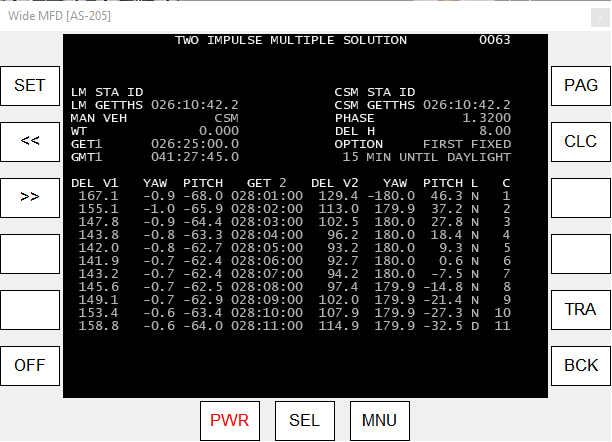
\includegraphics[width=0.8\textwidth]{./ApolloRTCCMFDFiles/TwoImpulseMultipleSolution.png}
	\caption{Multiple Solution Display}
	\label{fig:TwoImpulseMultipleSolution}
\end{figure}

\textbf{LM STA ID:} standard seven-character ID code indicating the LM anchor vector radar station at the time the display quantities were generated\\
\textbf{CSM STA ID:} same as above except for CSM\\
\textbf{LM GETTHS:} time tag of the vector from the current ephemeris table to be used in computing the maneuver, hr:min:sec\\
\textbf{CSM GETTHS:} same as above except for CSM\\
\textbf{MAN VEH:} maneuvering vehicle\\
\textbf{PHASE:} desired phase angle at the second maneuver, deg\\
\textbf{WT:} central angle of travel between the first and second maneuver, deg\\
\textbf{DEL H:} maneuvering vehicle\\
\textbf{GET1:} ground elapsed time of the fixed maneuver, hr:min:sec\\
\textbf{OPTION:} ID indicating whether the first, second, or both maneuver times are fixed\\
\textbf{GMT1:} Greenwich mean time of the first maneuver, hr:min:sec\\
\textbf{DAY/NIGHT INFO:} time until daylight or darkness for the fixed time maneuver, min\\
\textbf{DEL V1:} impulsive DV for the first maneuver, fps\\
\textbf{YAW:} yaw angle of the first maneuver, deg\\
\textbf{PITCH:} pitch angle above local horizontal of the first maneuver, deg\\
\textbf{GET2:} ground elapsed time of the variable maneuver, hr:min:sec\\
\textbf{DEL V2:} impulsive DV for the second maneuver, fps\\
\textbf{YAW:} yaw angle of the second maneuver, deg\\
\textbf{PITCH:} pitch angle above local horizontal of the second maneuver, deg\\
\textbf{TTPI:} With the special display logic explained above, the time of TPI is displayed instead of yaw and pitch of the second maneuver, hr:min:sec\\
\newpage
\paragraph{Corrective Combination (K32)}\mbox{} \\

\textbf{Inputs}:\\

\textbf{VEH:} Choose the chaser vehicle, CSM or LEM\\
\textbf{REQ:} Request type. 0 = second maneuver time incremented between the minimum and maximum times, 1 = second maneuver time is fixed\\
\textbf{CVT:} Chaser vector time. With the MPT inactive this option can be used to select the chaser vehicle\\
\textbf{TVT:} Target vector time. With the MPT inactive this option can be used to select the target vehicle\\
\textbf{NCC:} The time of the first maneuver (GET in hrs:min:sec)\\
\textbf{DHMIN:} Minimum target height offset at the second maneuver point (NM)\\
\textbf{DHMAX:} Maximum target height offset at the second maneuver point (NM)\\
\textbf{DHINC:} Height increment between minimum and maximum height offset (NM)\\
\textbf{T2MIN:} Minimum (mode 0) or actual (mode 1) time of the second maneuver (GET in hrs:min:sec)\\
\textbf{T2MAX:} Maximum time of the second maneuver for mode 0 (GET in hrs:min:sec)\\
\textbf{DT:} Time increment for incrementing the time of the second maneuver in mode 0 or for slipping TPI time in mode 1 (min)\\
\textbf{SLIP:} The amount by which TPI time is allowed to slip on either side of the nominal time for mode 1 (min)\\

\underline{NOTE}: If the mode designation is (1), thus fixing the second maneuver time at the input minimum time, TPI time is allowed to slip over the input range; whereas, if the mode designation is, (0), the time of the second maneuver is varied over its input range. For either mode, the time of the first maneuver is fixed, and the solution which requires the minimum DV for each height offset requested is displayed as the solution for that height.\\

\underline{NOTE}: The total DV (DVT) calculation for this display uses a curve fit to estimate TPI and TPF DVs. In this curve fit the terminal phase travel angle (WT) entered on the P51 MED is used. This is the WT on the multiple solution input page.\\

\textbf{P52:} Two-Impulse Corrective Combination Nominals. Input of the offsets is required for the corrective combination calculation. The inputs are the nominal time of NSR (GET in hrs:min:sec) and the nominal target height and phase angle offsets of NSR (NM and deg, respectively)
\newpage
\textbf{Display}:\\

\begin{figure}[hp]
	\centering
		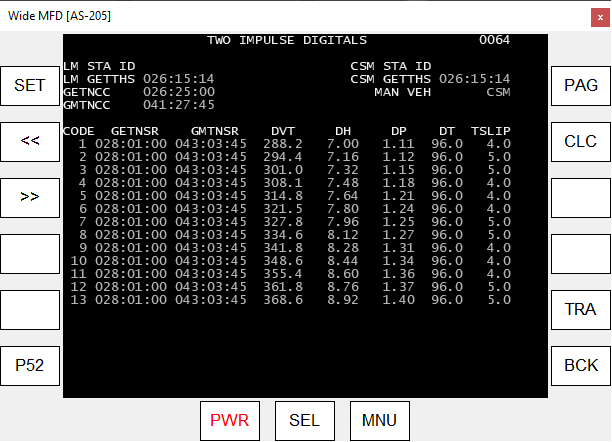
\includegraphics[width=0.8\textwidth]{./ApolloRTCCMFDFiles/TwoImpulseCorrectiveCombination.png}
	\caption{Corrective Combination Display}
	\label{fig:TwoImpulseCorrectiveCombination}
\end{figure}
\textbf{CSM STA ID:} Current CSM STA ID in MPT\\
\textbf{LM STA ID:} Current LM STA ID in MPT\\
\textbf{LM GETTHS:} time tag of the vector from the current ephemeris table to be used in computing the maneuver, hr:min:sec\\
\textbf{CSM GETTHS:} same as above except for CSM\\
\textbf{MAN VEH:} Maneuver vehicle code\\
\textbf{GETNCC:} Impulsive elapsed time of first maneuver of all solutions, hr:min:sec\\
\textbf{GMTNCC:} Impulsive GMT of same, hr:min:sec\\
\textbf{CODE:} Numeric code specifying the plan number of each solution in the table\\
\textbf{GETNSR:} Impulsive elapsed time of the second maneuver of the plane, hr:min:sec\\
\textbf{GMTNSR:} Impulsive GMT of same, hr:min:sec\\
\textbf{DVT:} Sum of the impulsive DVs for both maneuvers plus an approximation of the DV required for terminal phase\\
\textbf{DH:} Height offset after the second maneuver, NM\\
\textbf{DP:} Phase angle after the second maneuver, deg\\
\textbf{DT:} Time interval between first and second maneuvers, min\\
\textbf{TSLIP:} Amount of time terminal phase initiation will differ from the nominal if this solution is used, min\\
\newpage
\paragraph{Single Solution (K31)}\mbox{} \\

\textbf{Inputs}:\\

\textbf{TAB:} The two-impulse table indicator, either multiple solution or corrective combination\\
\textbf{SOL:} Solution number from that table (1 to 13)\\
\textbf{QUAD:} The number of RCS quads to be used in computing the burn times for the required DV components\\
\textbf{LOS:} The line-of-sight mode (i.e. whether the component DVs are in a body axes coordinate system defined by the astronauts line-of-sight aligned to the horizon or to the target vehicle)\\
\textbf{PIT:} The pitch angle (i.e. the angle between astronauts line-of-sight and the X body axis-deg)\\
\textbf{DT:} The time step between the relative motion data displayed (sec)\\

\textbf{Display}:\\
\begin{figure}[hp]
	\centering
		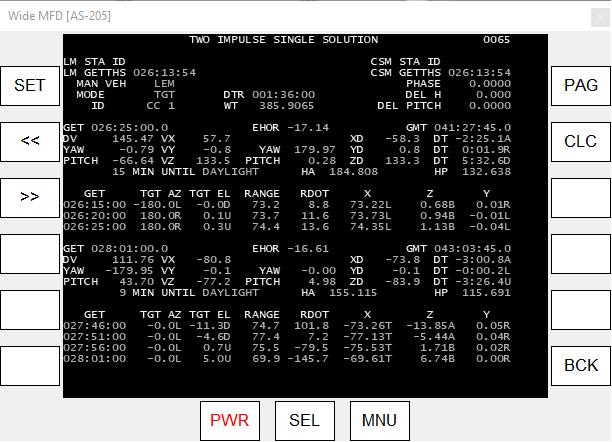
\includegraphics[width=0.8\textwidth]{./ApolloRTCCMFDFiles/TwoImpulseSingleSolution.png}
	\caption{Single Solution Display}
	\label{fig:TwoImpulseSingleSolution}
\end{figure}

\textbf{LM STA ID:} standard seven-character ID code indicating the LM anchor vector radar station at the time the display quantities were generated \\
\textbf{CSM STA ID:} same as above except for CSM\\
\textbf{LM GETTHS:} time tag of the vector from the current ephemeris table to be used in computing the maneuver, hr:min:sec\\
\textbf{CSM GETTHS:} same as above except for CSM\\
\textbf{MAN VEH:} Maneuver vehicle code\\
\textbf{PHASE:} actual phase lag at the second maneuver, deg\\
\textbf{MODE:} ID (either TGT or HOR) indicating the body-referenced coordinate system selected via input for the (XD, YD, ZD) DV definition defined below)\\
\textbf{DTR:} time between the two maneuvers, hr:min:sec\\
\textbf{DEL H:} actual differential altitude at the second maneuver time, NM\\
\textbf{ID:} code identifying the row number of the corresponding solution in the two-impulse multiple solution table or the two- impulse digital display\\
\textbf{WT:} central angle of travel of the target vehicle between maneuvers, deg\\
\textbf{DEL PITCH:} angle between the astronaut's line of sight (LOS) and the X-axis of the spacecraft (+ represents a counterclockwise rotation about the Y axis)\\
\textbf{GET:} ground elapsed time of the impulsive maneuver time, hr:min:sec\\
\textbf{EHOR:} angle between the astronaut's LOS to the horizon and the local horizontal plane, deg\\
\textbf{GMT:} Greenwich mean time of the impulsive maneuver time, hr:min:sec\\
\textbf{DV:} impulsive incremental velocity required by the maneuver, fps\\
\textbf{YAW} (on the left of display): yaw attitude relative to the local vertical/local horizontal (LVLH) reference frame at main engine ignition required to place the thrust vector along the DV vector (+ to the right), deg\\
\textbf{PITCH} (on the left of display): pitch attitude relative to the LVLH reference frame at main engine ignition required to place the thrust vector along the DV vector (+ up), deg\\
\textbf{VX, VY, VZ:} components of the incremental velocity along the X-, Y-, Z-axis, respectively, of either the target-defined or horizontal-defined body axis system, fps\\
\textbf{YAW} (in center of display): yaw angle between the X-axis of the (in center of display) spacecraft and the local horizontal
plane whenever the astronaut's LOS is to the target or the horizon, deg\\
\textbf{PITCH} (in center of display): pitch angle between X-axis of spacecraft and local horizontal plane whenever astronaut's LOS is to the target or horizon, deg\\
\textbf{XD, YD, ZD:} components of the incremental velocity along the X-, Y-, and Z-axis, respectively, of either the target-defined or horizontal-defined body axis system, fps\\
\textbf{DT} (associated with XD): burn time required to impart the velocity increment XD along the X-axis of the body axis system, by firing the fore or aft firing RCS thrusters, min:sec\\
\textbf{DT} (associated with YD): burn time required to impart the velocity increment YD along the Y-axis of the body axis system, by firing the left or right firing RCS thrusters, min:sec\\
\textbf{DT} (associated with ZD): burn time required to impart the velocity increment ZD along the Z-axis of the body axis system, by firing the up or down firing RCS thrusters, min:sec\\
\textbf{DAY/NIGHT INFO:} time until daylight or darkness for the fixed time maneuver, min\\
\textbf{HA:} apogee height after the maneuver, NM\\
\textbf{HP:} perigee height after the maneuver, NM\\
\textbf{GET:} ground elapsed time corresponding to the particular row of the approach data displayed, hr:min:sec\\
\textbf{TGT AZ:} azimuth of the target vehicle in the chaser vehicle's local vertical/local horizontal coordinate system, deg\\
\textbf{TGT EL:} elevation of the target vehicle in the chaser vehicle's local vertical/local horizontal coordinate system, deg\\
\textbf{RANGE:} range from the chaser to the target, NM\\
\textbf{R DOT:} range rate between chaser and the target, fps\\
\textbf{X, Y, Z:} position coordinates of the chaser vehicle in a target-centered curvilinear coordinate system, NM The letters L or T, R or L, and U or D are to be printed out with the position coordinates X, Y, and Z, respectively, to indicate whether the target vehicle is leading or trailing, to the right or to the left of, and above or below, the chaser vehicle\\
\newpage
\subsubsection{Coelliptic Maneuver Processor (SPQ)}

\paragraph{Explanation}\mbox{} \\

The Coelliptic Sequence Program computes the incremental velocities required to meet some relative vehicle positioning at the terminal phase initiation (TPI)
point. The maneuvers of the iterative sequence are the concentric sequence initiation maneuver (CSI) and the coelliptic maneuver (CDH), which may or may not be scheduled.\\

The desired relative positioning at TPI has two options: (1) that the active vehicle have a certain elevation angle to the target, or (2) that a desired differential altitude exist is the coelliptic orbit configuration.\\

The time of the CSI maneuver, if scheduled, is input. The desired CSI DV that will only be horizontal, may be computed with respect to a desired elevation
angle at TPI or a desired DH at CDH. An option exists to vary the CSI time within limits to reach both of these constraints.\\

There are five options for the computation of the CDH maneuver:
\begin{enumerate}
	\item Arrival at a next apsis (Integrator)
	\item At an input time
	\item After some desired travel angle from CSI
	\item Arrival at a next apsis (Keplerian)
	\item Number of half revolutions from CSI
\end{enumerate}

\paragraph{Buttons}\mbox{} \\

\textbf{INI:} Go to SPQ initialization page.\\
\textbf{VEH:} Choose which of the two vehicles is the chaser and which is the target.\\
\textbf{CHA:} Select the chaser vessel or the threshold time for the state vector of the chaser vehicle (MPT mode only).\\
\textbf{TGT:} Select the target vessel or the threshold time for the state vector of the target vehicle (MPT mode only).\\
\textbf{MOD:} Calculation mode, CSI or CDH maneuver or the optimum CSI mode which iterates on the CSI time to achieve both the desired DH at CDH and the desired time at TPI.\\
\textbf{TIM:} Switches between fixed GET and finding the delta height of the maneuver or fixed delta height and finding the time of ignition.\\
\textbf{TIG:} The time of the maneuver in GET. If the option is used to find the CDH time based on delta height this is an initial guess.\\
\textbf{CLC:} Calculate the burn solution.\\
\textbf{BCK:} Go back to the main menu.\\

\paragraph{Init page buttons}\mbox{} \\

\textbf{DH:} Delta height at the CDH maneuver.\\
\textbf{E:} Desired elevation angle at TPI.\\
\textbf{WT:} Desired travel angle between TPI and TPF.\\
\textbf{TPI:} Desired TPI time.\\
\textbf{CDH:} Select the option for the CDH maneuver point.\\
\textbf{VAL:} Select the defining value for the CDH maneuver point.\\
\textbf{BCK:} Go back to SPQ calculation page.\\
\paragraph{Display}\mbox{} \\

See Rendezvous Evaluation Display \ref{RED} under MOCR Displays.\\
\newpage

\subsubsection{Docking Initiation Processor (DKI)}

\paragraph{Explanation}\mbox{} \\

The basic function of the DKI is to compute impulsive maneuvers; the result of these maneuver is the rendezvous of the CSM and LM spacecraft. The DKI attains a coelliptic orbit by doing three maneuvers: (1) phase, (2) height, (3) a coelliptic maneuver that puts the chaser in a coelliptic orbit with the target. From this orbit a terminal phase maneuver (TPI) and a terminal velocity match maneuver (TPF) may be performed to achieve the actual rendezvous. The Skylab rendezvous sequences with an additional height maneuver is also supported.\\

The sequence of maneuvers are defined by so called maneuver lines. This terminology stems from the Gemini program. The first apogee after orbital insertion was assigned the number 1.0, the apogee one orbit later was maneuver line 2.0 and so forth. The Gemini 10 rendezvous for example had this maneuver schedule:

\begin{enumerate}
\item N=1.0: First apogee
\item N=1.5: Height maneuver (NH)
\item N=2.0: Phase maneuver (NC1)
\item N=3.0: Coelliptic maneuver (NSR)
\end{enumerate}

This results in the actual rendezvous (TPF) happening at roughly the fourth orbit after launch, in the Gemini terminology this was called M=4.\\

Terminology:\\

\begin{center}
\begin{tabular}{ p{1cm} p{10cm} }
M&The number of spacecraft apogee nearest the rendezvous point (M=4 is a fourth-apogee rendezvous)\\
N&The in-orbit maneuver line counter. Apogee point is N=X, perigee point is N=X.5, common nodal (plane change) points are N= X.25 or X.75\\
NH&Apogee height adjustment maneuver performed at perigee end of maneuver line. NH = 1.5 denotes height adjustment near first spacecraft perigee\\
NC1&Phase adjustment maneuver performed at apogee end of maneuver line to change the catch-up rate. NC1 = 2 denotes phase adjustment near second spacecraft apogee.\\
\end{tabular}
\end{center}

\paragraph{TIG and TPI Definition}\mbox{} \\

On this page the time of ignition and time of the TPI maneuver are defined.

\textbf{VEH:} Choose the active vehicle for the rendezvous. Options are CSM or LM. The MFD automatically detects if the current vehicle is a CSM or not.\\
\textbf{PRO:} For the Skylab rendezvous profile with an additional height adjustment maneuver this option can be set, otherwise the Regular DKI option should be used.\\
\textbf{MAN:} Options for the initial maneuver line. The line can be defined for an input time, chaser apoapsis or target apoapsis. Input time is useful if the time of ignition or number of orbits to time of ignition is given. Chaser apoapsis is the typical option for ground-up Earth orbit rendezvous. Should the target be in an elliptical orbit the target apoapsis option is useful to keep the maneuver line near the line-of-apsides of the targeting, which prevents large vertical Delta V components for the coelliptic maneuver.\\
\textbf{ML:} Value of the initial maneuver line. This can be chosen arbitrarily, but usually an X.0 value is assigned to a chaser apoapsis. Another example is a CSM rescue maneuver in lunar orbit, which is supposed to happen one orbit after DOI. Then the time of DOI is used for the initial maneuver line, the value entered with this button should be 1.0 and then first maneuver should be scheduled at the 2.0 maneuver line point\\
\textbf{PHA:} Flag to describe the initial phase angle. Normally set to 0 to indicate a phase angle of -180 to 180 DEG. In this case the chaser needs to catch up if it is behind the target by e.g. 10 DEG. If the chaser is ahead of the target by 10 DEG it needs to slow down, which means a higher orbit. If the flag is set to -1 in the first case the phase angle is interpreted as -350 DEG instead of 10 DEG and the chaser will slow down, go into a higher orbit, to achieve rendezvous. This is mainly useful for rendezvous sequences that take many orbits.\\

\textbf{TPD:} Definition of the terminal phase. There are three options for both TPI and TPF, so in total six combinations. The three options are input time, time from sunrise and time from sunset. Usually the time of TPI is known from an external calculation or the time from sunrise option with a negative time is used, to set the TPI maneuver in darkness at a fixed time before sunrise.\\
\textbf{TPV:} Input value associated with the terminal phase definition. Either a GET or a time in minutes from sunset or sunrise.\\

\paragraph{Init Parameters}\mbox{} \\

\textbf{DH1:} The Delta Height at the NCC maneuver point. Only required for Skylab rendezvous profile. Usually 20 NM\\
\textbf{DH2:} The Delta Height at the NSR maneuver point. A positive value indicates the chaser vehicle being below the target. Usually 10 to 20 NM.\\
\textbf{E:} Elevation angle at TPI. Typical value is 26.6 DEG for a rendezvous from below. For rendezvous from above, for example if the CSM needs to rescue the LM in lunar orbit, the value 208.3 DEG is usually used.\\
\textbf{WT:} Transfer angle from TPI to TPF, typically between 130 and 140 degrees.\\
\textbf{MIN:} Minimum allowable periapsis altitude in the rendezvous plan.\\

\paragraph{DKI Inputs}\mbox{} \\

\textbf{NC1:} Choose the maneuver line number of the NC1 maneuver. Set to a negative value if no phasing maneuver is in the maneuver plan.\\
\textbf{NH1:} Choose the maneuver line number of the NH maneuver. Set to a negative value if no height maneuver is in the maneuver plan.\\
\textbf{NSR:} Choose the maneuver line number of the NSR maneuver. If the rendezvous profile is the Skylab profile then the NCC maneuver line number is selected here and NSR happens at a specific time after NCC.\\
\textbf{MI:} The maneuver line number for the rendezvous point (TPF). This is an integer number and only has to be a rough estimate, typically this will be set so that rendezvous occurs one orbit after NSR.\\
\textbf{IDM:} Number of additional rendezvous plans that are being generated. For this the NSR and subsequent maneuvers are set to occur one orbit later and the DKI calculation is run again for the updated plan.\\
\textbf{MNH:} Location of the NH maneuver in the additional plans select with the IDM button. The NH maneuver either stays at its original maneuver line, as specified on this MFD page, or it is being moved one orbit for every additional plan, in effect keeping its place in the plan relative to NSR.\\
\textbf{NPC:} Location of the plane change maneuver in the rendezvous plan. Not available yet.\\
 
\paragraph{Example: Apollo 10 PDI Abort}\mbox{} \\

A simple example for a DKI targeted maneuver is the Apollo 10 PDI Abort. Similar in concept to the PDI+12 maneuvers of the lunar landing missions, Apollo 10 would have done an abort maneuver at perilune after DOI to return to the CSM one orbit earlier than in the normal rendezvous plan. The sequence of maneuvers would be the abort initiation 0.5 revolutions after DOI, targeted as a phasing (NC1) maneuver. CSI or NH would follow another half revolution later, and again the CDH or NSR maneuver would be half an orbit after that. If we assign 1.0 as the maneuver line to the DOI maneuver then we would have NC1 = 1.5, NH = 2.0, NSR = 2.5, M = 3. The maneuver line definition is using the time option with the DOI TIG as input.

\newpage
\subsection{General Purpose Maneuver (GPM)}

\subsubsection{Explanation}

The following explanation was taken from IBM RTCC Apollo Programming Systems, Missions Systems, General, Volume II (NTRS ID 19730062603):

The function of the General Purpose Maneuver Processor is to provide the flight controller with two main capabilities:

\begin{enumerate}
	\item To determine the effect that a specified incremental velocity applied at a given maneuver point (along a given pitch and yaw) will have on the orbit.
	\item To determine the maneuver required to obtain a specified orbit or orbital change.
\end{enumerate}

The first capability is more commonly known as a flight controller special-maneuver request and has six options for the maneuver point:

\begin{enumerate}
	\item An equatorial (nodal) crossing
	\item A specified longitude
	\item A specified time
	\item A specified height
	\item An apogee crossing
	\item A perigee crossing
\end{enumerate}

The second capability is divided into eight types with various maneuver points:

\begin{enumerate}
	\item A plane change at a certain equatorial crossing, longitude, time, or height.
	\item A circularization maneuver at a longitude or height.
	\item A maneuver at perigee to adjust apogee or vice-versa.
	\item A maneuver to adjust the height 180$^{\circ}$ around from the maneuver point at a longitude or time.
	\item A maneuver to shift the ascending node at an optimum time, longitude, time or height.
	\item A maneuver to obtain a specified apogee and perigee at an optimum time, longitude, or height.
	\item A maneuver to shift the ascending node and adjust the height 180$^{\circ}$ around from the maneuver point at a longitude or time.
\item A maneuver to shift the line of apsides to the maneuver point and obtain a specified height 180$^{\circ}$ around from the maneuver point at a time, longitude, or height.
\end{enumerate}

The output from the GPM Processor is a display containing such maneuver information as DV, pitch, yaw, maneuver time, maneuver height, etc., and such post maneuver information as apogee and perigee heights, longitude of the ascending nodes, eccentricity, etc. A table containing the elements before and after the maneuver at the impulsive time is also output so the maneuver may be transferred to the Mission Plan Table, if desired.\\

\subsubsection{Buttons}

\textbf{SET:} Make an input for the GPM processor.\\
\textbf{<<:} Move the marker down.\\  
\textbf{>>:} Move the marker up.\\
\textbf{CLC:} Calculate the maneuver.\\
\textbf{MPT:} Create finite maneuver from impulsive burn.\\
\textbf{BCK:} Go back to the main menu.\\
\newpage
\subsection{TLI Planning}
\subsubsection{Introduction}
On a typical lunar mission all the targeting needed for TLI has been loaded into the Saturn computer (LVDC) before launch. For a dispersed Earth orbit or an alternative mission the RTCC has the capability to target a new TLI or an alternative second S-IVB burn. The options available in the TLI processor are

\begin{enumerate}
	\item S-IVB hypersurface solution. Evaluates the preloaded targeting in the LVDC
	\item Integrated free-return trajectory to the nominal lunar flyby conditions
	\item Specified total Delta V
	\item Specified apogee altitude
	\item Integrated non-free return trajectory to the nominal nodal position at the Moon
	\item External Delta V
\end{enumerate}

\subsubsection{Inputs}
\textbf{IU:} Select the vessel that is used for the uplink of the updated TLI targeting. In non-MPT mode also used as the vessel from which the state vector and weights are taken for the TLI processor calculation.\\
\textbf{MPT:} Select CSM or LM mission plan table (MPT mode only).\\
\textbf{VEC:} Select the state vector used in the calculation. Normally the anchor vector of the CSM or LM ephemeris is used, but any vector in the useable vector table can be specified (MPT mode only).\\
\textbf{Opp:} Select the TLI opportunity. For option 1 this is the input to choose when the TLI is done and for all options this changes certain parameters associated with one of the opportunities in the LVDC, mostly the time of S-IVB mixture ratio shift from ignition.\\
\textbf{Mode:} Choose the TLI processor calculation mode, see list above.\\
\textbf{TIG:} Time of ignition. Not used for option 1. Used as a very rough initial guess in option 2 and 5, that only has to be accurate to a full orbit. In options 3 and 4 this is the exact time of ignition used.\\
\textbf{DV:} Delta V of the maneuver (option 3) or Delta V vector (option 6).\\
\textbf{APO:} Apogee altitude to be achieved by the maneuver (option 4 only).\\
\textbf{Window:} Pacific or Atlantic TLI window, for the lunar mission options (2 and 5) this is used to generate the initial guess.\\
\textbf{SFP:} For the lunar mission options (2 and 5) the target parameters are taken from the Skeleton Flight Plan table, which has two sets of data. See the Midcourse Correction Processor for more details about the SFP.\\

\textbf{CLC:} Calculate solution.\\
\textbf{MPT:} Transfer maneuver to MPT.\\
\textbf{UPL:} Uplink solution to IU.\\
\newpage
\subsubsection{Display}

\begin{figure}[hp]
	\centering
		\includegraphics{./ApolloRTCCMFDFiles/TLIProcessorDisplayExample.png}
	\caption{TLI Planning Display}
	\label{fig:TLIProcessorDisplayExample}
\end{figure}

\textbf{Display Parameters}\\

\textbf{GET RP:} Ground Elapsed Time of Restart Preparations (TB6)\\
\textbf{GET TIG:} Ground Elapsed Time of main engine ignition\\
\textbf{INCL:} Inclination at cutoff\\
\textbf{DESC:} Longitude of the descending node at cutoff\\
\textbf{ECC:} Eccentricity at cutoff\\
\textbf{C3:} Orbital energy at cutoff\\
\textbf{ALPHA:} Angle from perigee of cutoff ellipse to descending node of cutoff ellipse\\
\textbf{TA:} True anomaly at cutoff\\
\textbf{BT:} Burn time of maneuver\\
\newpage
\subsection{Midcourse Correction Processor}

\subsubsection{Introduction}

During the translunar coast phase of an Apollo mission, it is necessary to have the capability to either correct dispersions in the nominal trajectory or determine an alternate flight plan which is within the capability of the spacecraft. This capability is provided by the midcourse correction processor. The processor has the ability to correct a dispersed state vector to some nominal end conditions, reoptimize the lunar landing mission, and generate a circumlunar flyby alternate mission. The computation types to obtain these requirements are:

\begin{enumerate}
	\item The x, y, z, and t target update (XYZ midcourse mode).
	\item The best adaptive path (BAP) reoptimization.
	\item The free-return lunar flyby mode.
\end{enumerate}

One or more mission options are available under each mode. The mission options, listed below, are defined by their mode, type of return, lunar parking orbit (LPO) orientation, and whether the mission is tied to a landing site.

\begin{enumerate}
	\item X, Y, Z and T target update.
	\item Free-return, fixed LPO orientation, landing site.
	\item Free-return, free LPO orientation, landing site.
	\item	Nonfree-return, fixed LPO orientation, landing site
	\item	Nonfree-return, free LPO orientation, landing site
	\item	Circumlunar free-return flyby to nominal H\textsubscript{pc} and $^{\phi}$\textsubscript{pc}
	\item	Circumlunar free-return flyby, specified H\textsubscript{pc} and nominal $^{\phi}$\textsubscript{pc}
	\item	SPS lunar flyby to specified H\textsubscript{pc} and INCL\textsubscript{fr}
	\item	Optimized RCS flyby to desired or optimal inclination of free return
\end{enumerate}

The MCC processor implemented in the RTCC MFD presents the last state of the processor, as used for Apollo 14 through the end of the program. Certain procedural differences for using the processor with the earlier missions arise from this, but all lunar Apollo missions are fully supported.

\subsubsection{Input/Output}

Inputs for all midcourse modes fall into two categories: those from the data table (also called skeleton flight plan), and those which are manually entered during the mission by the user. The data table contains variables which are needed to execute the different options. These variables may be target parameters used in the XYZ and T mode or first guesses for certain variables. The table also contains parameters which change according to the nominal mission design and launch day (e.g., the lunar landing site). Output parameters from a BAP midcourse can be used to update the data table for later midcourse calculations or the XYZ and T midcourse mode. The data table and the manual inputs are defined in table I and II.\\

Output from the MCC program are of three types: those displayed, those that are needed for executing the midcourse maneuver, and those which update the data table. Displayed parameters are shown in table III. Output for the data table is shown in table I. BAP’s are the only options that update the data table.\\

In the RTCC MFD the MCC processor consists of three display pages: computational inputs, constraints on the solutions and the MCC tradeoff display (modelled after the real display used in Mission Control Houston). On the constraints page some of the inputs are made in the MED format (Manual Entry Device), which is the same format as was used in the real RTCC. The MEDs for the midcourse processor all have codes starting with an F, e.g. F22. The MED inputs are checked for errors and certain omissions are replaced by default values.\\

\subsubsection{SFP page}

The SFP page contains the skeleton flight plan table (SFP) parameters that are inputs and outputs for the midcourse processor. Usually only one operation has to be done on this page for a nominal mission. Before any midcourse maneuver can be calculated, the initial SFP (Called the preflight table) has to be interpolated from tables that are valid for the whole daily launch window. This is accomplished by using the F62 button and entering the TLI opportunity (1 or 2) and the launch azimuth (usually but not always 72 degrees). The input format is: F62,,1,72.0; The launch day is an optional parameter that could be entered after the first comma, but is usally not needed. Once the F62 MED was entered the SFP table should populate with numbers. Afterwards the MCC processor can be used for calculations.

\subsubsection{Computation page}

\textbf{MAN:} Maneuver option (1 to 9), see description above.\\
\textbf{VTI:} Vector time. Time tag of the state vector from the ephemeris (mission planning mode only).\\
\textbf{IG:} Impulsive time of ignition of the midcourse maneuver.\\
\textbf{COL:} Column for the solution. The Midcourse Tradeoff display can hold up to 4 different solutions from the MCC processor.\\
\textbf{CFG:} Configuration for the midcourse maneuver, options are docked or undocked. Used to calculate certain display parameters only.\\
\textbf{SFP:} Skeleton flight plan (data table) used for initial guesses and target parameters. Table 1 usually contains the preflight data, table 2 the results of a previous BAP midcourse calculation that were transferred from the midcourse tradeoff. Tables 3 to 5 will be supported in the future.\\
\textbf{MID:} Go to midcourse tradeoff display MFD page.\\
\textbf{HPC:} Pericynthion altitude for lunar flyby modes.\\
\textbf{INC:} Free return inclination for lunar flyby modes 8 and 9. Mode 9 is further divided into mode 9A (RCS optimized flyby) and 9B (SPS optimized flyby to specified free return inclination). If the input inclination is 0, then mode 9A, the fully optimized flyby, will be used. Otherwise the specified inclination is attained. By using a plus or minus sign for the inclination an ascending or descending return can be specified (travelling from south to north and north to south at reentry respectively).\\
\textbf{CON:} Go to midcourse constraints MFD page.\\
\textbf{BCK:} Go back to previous menu.\\

\subsubsection{Constraints page}

\textbf{F22:} Azimuth constraints. Input method: “F22, Minimum Azimuth,Maximum Azimuth;” Limited to -110° to -70°. Used by modes 3 and 5. Constrains the approach azimuth to the landing site at the time of landing. Special logic is used if the min and max azimuths are set the identical. In that case the lunar orbit has a fixed orientation, although without imposing the LOI/DOI geometry. This should be done for missions which used the LOI-1/LOI-2 maneuver sequence (Apollo 8,10-12). Example: F22,-90,-90;\\
\textbf{F23:} Time constraints. Input method: “F23,TLMIN,TLMAX;” Used by modes 4-5. This sets a minimum or maximum time limit for the arrival at pericynthion. Useful for missions with stricter timing requirements for arriving in lunar orbit (Apollo 14 to 17). If ommited (input: “F23;”) The constraints are zeroed and the pericynthion time is not constraint.\\
\textbf{F24:} Reentry constraints. Input method: “F24,Flight Path Angle,Reentry Range;” Used in the free return and lunar flyby modes. Inputs are the flight path angle at entry interface and the range from entry interface to landing.\\
\textbf{F29:} Pericynthion height limits. Input method: “F29,HPMIN,HPMAX;” Used in mode 9 only. Can be used to force the solution indirectly to a different splashdown longitude.\\
\textbf{LAT:} Latitude bias for modes 8 and 9. TBD\\
\textbf{INC:} Maximum inclination for the powered return (TEI). Not enforce yet.\\
\textbf{LOI:} Apolune and perilune height of the LOI (LOI-1) ellipse.\\
\textbf{DOI:} Apolune and perilune height of the DOI (LOI-2) ellipse.\\
\textbf{REV:} Input: REVS1 REVS2. Number of orbits spent in the first (LOI to DOI/LOI-2) and second (DOI/LOI-2 to landing site) lunar orbit. REVS2 is always an integer, REVS1 can contain partial orbits.\\
\textbf{ROT:} Input: SITEROT ETA. The first parameter is the true anomaly at the landing site at the time of landing. Usually PDI should happen at perilune, which will be 15° ahead of the landing site. In that case 15 should be the input. ETA is the true anomaly of LOI on the post LOI orbit. This will usually be consistent with the REVS1 parameter, which will put DOI at perilune.\\
\textbf{PC:} Revolutions before and after the lunar orbit plane change maneuver. Used to estimate the trajectory in lunar orbit. The first parameter M is the number of orbits between the lunar landing and the plane change maneuver. The parameter N is the number of orbits between the plane change and lunar ascent.\\
\textbf{BCK:} Back to midcourse calculation page.\\
\newpage
\subsubsection{Midcourse Tradeoff Display}

\begin{figure}[h]
	\centering
		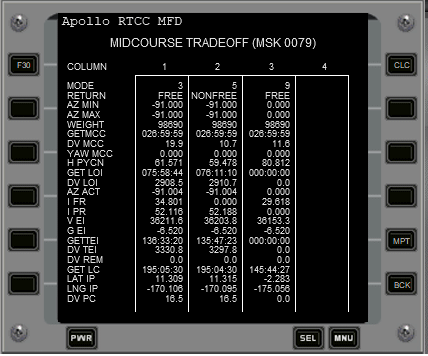
\includegraphics{./ApolloRTCCMFDFiles/RTCCMFD_MCC_Modes_359.png}
	\caption{Midcourse Tradeoff Display}
	\label{fig:RTCCMFD_MCC_Modes_359}
\end{figure}

\textbf{COLUMN:} Shows up to 4 midcourse correction solutions.\\
\textbf{MODE:} Shows the mode (1-9) that was calculated.\\
\textbf{AZ MIN:} Minimum approach azimuth at the landing site.\\
\textbf{AZ MAX:} Maximum approach azimuth at the landing site.\\
\textbf{WEIGHT:} Weight at ignition in lbs.\\
\textbf{GETMCC:} Estimated time of ignition of the midcourse correction (actual, not impulsive).\\
\textbf{DV MCC:} Total DV of the midcourse correction in feet per second.\\
\textbf{YAW MCC:} Yaw angle (out-of-plane) of the maneuver.\\
\textbf{H PYCN:} Height of pericynthion resulting from the maneuver.\\
\textbf{GET LOI:} Estimated time of ignition of LOI (actual, not impulsive).\\
\textbf{DV LOI:} Total DV of LOI maneuver.\\
\textbf{AZ ACT:} Actual approach azimuth at the landing site.\\
\textbf{I FR:} Free return inclination, Earth referenced.\\
\textbf{I PR:} Powered return (TEI) inclination, Earth referenced.\\
\textbf{V EI:} Velocity at entry interface in feet per second.\\
\textbf{G EI:} Flight path angle (gamma) at entry interface.\\
\textbf{GETTEI:} GET of the TEI maneuver.\\
\textbf{DV TEI:} Total DV of the TEI maneuver.\\
\textbf{DV REM:} DV remaining after TEI (not implemented).\\
\textbf{GET LC:} GET of splashdown.\\
\textbf{LAT IP:} Latitude of splashdown (impact point).\\
\textbf{LNG IP:} Longitude of splashdown (impact point).\\
\textbf{DV PC:} Total DV of lunar orbit plane change maneuver.\\
\newpage
\subsection{Lunar Orbit Insertion (LOI) Processor}

\subsubsection{Introduction}

The LOI processor calculates the LOI-1 maneuver for an Apollo lunar mission. The maneuver is targeted based on the following assumed trajectory profile to the landing site. All plane change is accomplished with the first burn. A second burn (LOI-2 or DOI) adjusts the inplane orbital elements so that a specified orbit occurs at the landing site. It is not not always possible to meet all desired end conditions; thus various solutions are computed.

There are four solution types, each with a positive-negative solution, for a total of eight solutions. A positive solution is one whose perilune is rotated ahead (i.e., in the direction of motion); a negative solution is one whose perilune is rotated behind (i.e., opposite to the direction of motion). The four types are as follows.

\begin{itemize}
	\item Plane solutions: obtain the desired azimuth at the landing site, giving up the lunar orbit perilune if necessary, which is if the node between the incoming trajectory (approach hyperbola) and the orbit after LOI occurs at an altitude below the desired perilune, or above the desired apolune. This is the type of LOI maneuver generally used for Apollo 12 and earlier.
\item Coplanar solutions: obtain the desired lunar orbit shape (apolune and perilune) in the plane of the approach hyperbola with a pre-hyperbolic perilune impulsive point for the positive solution and a post-hyperbolic perilune impulsive point for the negative solution. This solution type therefore has no plane change.
\item Minimum Theta solutions: obtain the desired lunar orbit shape (apolune and perilune) and minimize the wedge angle between the actual and desired lunar orbit plane within an input maximum allowable DV.
\item Intersection solutions: adjusts the first lunar orbit perilune altitude to obtain a specified altitude difference (or intersection with no altitude difference) between it and the altitude on the post-DOI lunar orbit. This is the type of LOI maneuver generally used for Apollo 13 and later and has no use if the second lunar orbit maneuver (LOI-2) is a circularization maneuver.
\end{itemize}

The LOI processor implemented in the RTCC MFD is based on the one used for Apollo 14 and later. Most capabilities of earlier programs are retained, so that all lunar missions are still supported.
\newpage

\subsubsection{Inputs}

The inputs for the LOI processor are divided in initialization parameters and computation parameters.\\

\textbf{Computation Parameters}

\textbf{INI:} Got to LOI initialization page.\\
\textbf{VTI:} Time for taking the state vector from the CSM ephemeris (MPT mode only).\\
\textbf{APO:} Apolune height after LOI.\\
\textbf{PER:} Perilune height after LOI.\\
\textbf{DVP:} Maximum DV for positive Min Theta solution.\\
\textbf{DVN:} Maximum DV for negative Min Theta solution.\\
\textbf{DIS:} Got to LOI display.\\
\textbf{AMN:} Choose the minimum approach azimuth to the landing site.\\ 
\textbf{ADS:} Choose the desired approach azimuth to the landing site.\\ 
\textbf{AMX:} Choose the maximum approach azimuth to the landing site.\\
\textbf{BCK:} Back to main menu.\\

\textbf{Initialization Parameters}

\textbf{HA:} Apolune height after DOI/LOI-2.\\
\textbf{HP:} Perilune height after DOI/LOI-2.\\
\textbf{DW:} Angle of perilune from the landing site (negative if the landing site is post-perilune).\\
\textbf{R1:} Number of revolutions in the first lunar orbit (may have a fractional part).\\
\textbf{R2:} Number of revolutions in the second lunar orbit.\\
\textbf{ETA:} True anomaly of LPO-1 for transferring from the hyperbola to LPO-1.\\
\textbf{DHB:} Altitude constraint of the intersection solutions. The bias is negative if LPO-2 is to be below the LPO-1 perilune.\\
\textbf{PLA:} A flag to specify if plane or minimum Theta nodes should be used to compute intersection solutions.\\
\textbf{BCK:} Back to LOI computation page\\ 
\newpage
\subsubsection{LOI Display}

This display is based on the actual display used by the flight controllers for Apollo 14.\\

\begin{figure}[hp]
	\centering
		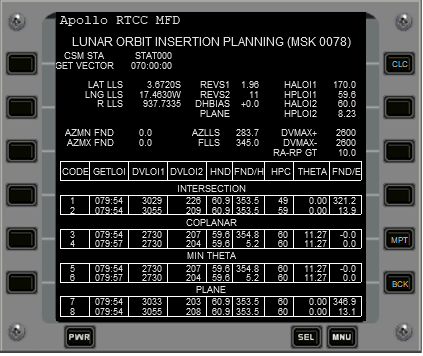
\includegraphics{./ApolloRTCCMFDFiles/RTCCMFDLOIDisplayApollo14Example.png}
	\caption{LOI Planning Display}
	\label{fig:RTCCMFDLOIDisplayApollo14Example}
\end{figure}

\textbf{Display Parameters}\\
\textbf{CSM STA:} Station ID of the state vector used to target the maneuvers (not implemented).\\
\textbf{GET VECTOR:} GET of state vector used to target LOI.\\
\textbf{LAT LLS:} Latitude of the landing site in degrees.\\
\textbf{LNG LSS:} Longitude of the landing site in degrees.\\
\textbf{R LLS:} Radius of the landing site in nautical miles.\\
\textbf{REVS 1:} Revolutions in LPO-1.\\
\textbf{REVS 2:} Revolutions in LPO-2.\\
\textbf{DH BIAS:} Height bias for the intersection solutions.\\
\textbf{AZ LLS:} Desired azimuth at the landing site.\\
\textbf{FLLS:} Angle of perilune from the landing site.\\
\textbf{HALOI1:} Apolune height on first lunar orbit.\\
\textbf{HPLOI1:} Perilune height on first lunar orbit.\\
\textbf{HALOI2:} Apolune height on second lunar orbit.\\
\textbf{HPLOI2:} Perilune height on second lunar orbit.\\
\textbf{DVMAX+:} Maximum allowable DV for the positive Min Theta solution.\\
\textbf{DVMAX-:} Maximum allowable DV for the positive Min Theta solution.\\
\textbf{RA-RP GT:} Tolerance for the calculation of DVLOI2 in nautical miles.\\

\textbf{CODE:} Code for the eight possible solutions.\\
\textbf{GETLOI:} Impulsive GET of LOI ignition.\\
\textbf{DVLOI1:} Total DV of LOI-1 in feet per second.\\
\textbf{DVLOI2:} Total DV of DOI/LOI-2 in feet per second.\\
\textbf{HND:} Height of the node (impulsive LOI ignition point).\\
\textbf{FND/H:} True anomaly at LOI on the approach hyperbola (pre LOI).\\
\textbf{HPC:} Height of perilune on the first lunar orbit.\\
\textbf{THETA:} Angle between the desired lunar orbit plane and the actual achieved plane.\\
\textbf{FND/E:} True anomaly at LOI on the first ellipse (post LOI).\\
\newpage
\subsection{Lunar Descent Planning Processor}
The LDPP computes maneuver sequences to be executed by the CSM and the LM to yield a set of desired orbital conditions at the point of LM descent ignition or a desired CSM orbital plane at the time of LM liftoff. There are seven modes of operations from which to choose. Each of these modes may contain more than one sequence. Each sequence may or maybe not have more than one maneuver. The following table presents a list of maneuver sequences in each mode:\\

\begin{center}
\begin{tabular}{|l|l|l|l|l|l|l|}
\hline
Mode&Maneuver&\multicolumn{5}{|l|}{Sequence}\\
\hline
&&1&2&3&4&5\\
\hline
1&1&PC&PCC&ASP&PCCH&PCCT\\
&2&DOI&DOI&CIA&DOI&DOI\\
&3&--&--&DOI&--&--\\
\hline
2&1&ASH&CIR&--&--&--\\
&2&DOI&DOI&--&--&--\\
\hline
3&1&ASH&--&--&--&--\\
&2&CIA&--&--&--&--\\
&3&DOI&--&--&--&--\\
\hline
4&1&DOI&--&--&--&--\\
\hline
5&1&PC&HO1&HO1&--&--\\
&2&HO1&PC&HO2&--&--\\
&3&HO1&HO2&PC&--&--\\
&4&DOI&DOI&DOI&--&--\\
\hline
6&\multicolumn{4}{|l|}{Go to powered descent}&--&--\\
\hline
7&1&PPC&&&--&--\\
\hline
\end{tabular}
\end{center}

Abbreviations:\\

\begin{center}
\begin{tabular}{l l}
ASP&Apside shift, altitude adjustment, and plane change maneuver\\
ASH&Apside shift and altitude adjustment maneuver\\
CIA&Circularization at an apsis maneuver\\
CIR&Circularization maneuver\\
DOI&Descent orbit injection maneuver\\
HO1&First maneuver in a double Hohmann sequence\\
HOI2&Second maneuver in a double Hohmann sequence\\
PC&Plane-change maneuver\\
PCC&Plane change and circularization maneuver\\
PCCH&Plane change and circularization maneuver at a desired height\\
PCCT&Plane change and circularization maneuver at a desired time\\
PPC&Prelaunch plane-change maneuver\\
\end{tabular}
\end{center}
\newpage
Detailed description of each mode:\\
\begin{center}
\begin{tabular}{l l l m{7.3cm}}
Maneuver&Maneuver&Maneuver&\\
Mode No.&Sequence No.&Display Code& Definition\\
\hline
1&1&PC&Compute plane-change maneuver only\\
\hline
1&2&PCC&Compute plane-change and circularization maneuver\\
\hline
1&3&ASP-CIA&Compute plane-change maneuver combined with first maneuver of a CSM two maneuver sequence to circularize the CSM orbit at an input altitude\\
\hline
1&4&PCCH&Compute plane-change and circularization maneuver at a specific altitude\\
\hline
1&5&PPCT&Compute plane-change and circularization maneuver at an input time\\
\hline
2&2&ASH&Compute CSM maneuver to establish an apsis and an input altitude at the DOI maneuver point\\
\hline
2&3&CIR&Compute CSM maneuver to circularize orbit at an input altitude\\
\hline
3&1&ASHT-CIA&Compute CSM two-maneuver sequence with the first maneuver performed at an input time and the second maneuver performed at an input altitude to circularize the orbit\\
\hline
3&3&ASHA-CIA&Compute CSM two-maneuver sequence with the first maneuver performed at an apsis and the second maneuver performed at an input altitude to circularize the orbit\\
\hline
\end{tabular}
\end{center}
\newpage
\begin{center}
\begin{tabular}{l l l m{7.3cm}}
Maneuver&Maneuver&Maneuver&\\
Mode No.&Sequence No.&Display Code& Definition\\
\hline
4&1&DOI&Computes the DOI maneuver only\\
\hline
4&2&DOI&Computes the DOI maneuver only and includes a plane change\\
\hline
4&3&DOI&Computes the DOI maneuver with a higher fidelity numerical integration processor, for a more precise perilune altitude and placement. Useful for CSM DOIs that take place many hours before PDI.\\
\hline
4&4&DOI&Same as sequence 3, but with an included plane change.\\
\hline
5&1&PC, HO1, HO2&Compute CSM three-maneuver sequence so that the first maneuver is a plane change and the following pair is a double Hohmann to a circular orbit at an input altitude\\
\hline
5&2&HO1, PC, HO2&Compute CSM three-maneuver sequence so that the first maneuver initiates a double Hohmann, the second is a plane-change, and the third completes  the double Hohmann to a circular orbit at an input altitude\\
\hline
5&3&HO2, HO2, PC&Compute CSM three-maneuver sequence so that the first two maneuvers constitute a double Hohmann to a circular orbit at an input altitude and the third is a plane change\\
\hline
6&1&PDI&Powered descent only\\
\hline
7&1&PPC&Prelaunch plane change\\
\hline
\end{tabular}
\end{center}
\newpage
\subsubsection{Initialization Parameters}
\begin{center}
\begin{tabular}{ | m{1cm} | m{4cm} | m{8.5cm} |}
\hline
Button&Parameter&Description\\
\hline
AZI&Approach azimuth&For the calculation modes that involve a plane change maneuver, the approach azimuth to the landing site can be specified. If this is not required then the parameter can be set to 0, which will result in the optimum (smallest) plane change burn to be calculated\\
\hline
HDP&Altitude of point of descent ignition&Usually the DOI maneuver will set up PDI to occur at this specific altitude\\
\hline
PDS&Powered-descent simulation flag&Set to perform a a detailed simulation of powered descent (not implemented yet)\\
\hline
PDI&Powered-descent time&If the powered descent is to be simulated, this option either lets you choose the time of PDI or let it be internally calculated. For this the time should be set to zero\\
\hline
N&Dwell orbits&Number dwell orbits desired between DOI and powered-descent ignition\\
\hline
DFT&Descent flight time&Time from PDI to touchdown\\
\hline
DFA&Descent flight arc&Travel angle from PDI to touchdown. Usual values are 15 to 16 degrees\\
\hline
LSO&Landing site offset&Usually this will be set to the same value as DFA. This will cause PDI to occur at perilune. If PDI is desired to occur at a different point in the orbit, like on Apollo 17, then this value can control where the perilune will be located relative to the landing site. A value of -10 degrees will have the perilunar location 10 degrees after landing site passage\\
\hline
\end{tabular}
\end{center}
\newpage
\subsubsection{Computation Parameters}

\begin{center}
\begin{tabular}{ | m{1cm} | m{4cm} | m{8.5cm} |}
\hline
VEH&Vehicle&Select if CSM or LM are performing the maneuver sequence\\
\hline
VTI&Vector time&With MPT enable, this time is the vector time from the ephemeris. Otherwise it seconds as a vehicle selection button\\
MOD&Mode&Select the calculation mode (1-7)\\
\hline
SEQ&Sequence&Select the specific maneuver sequence\\
\hline
HEI&Height&Altitude wanted at apsis. Typically the altitude at which DOI is desired to occur, but depending on the mode can also be the circularization maneuver altitude\\
\hline
TH1&Threshold time 1&Threshold time for the first maneuver of a sequence\\
\hline
TH2&Threshold time 2&Threshold time for the second maneuver of a sequence\\
\hline
TH3&Threshold time 3&Threshold time for the third maneuver of a sequence\\
\hline
TH4&Threshold time 4&Threshold time for the fourth maneuver of a sequence. DOI maneuvers will always use this time as the threshold for the maneuver. For a prelaunch plane-change maneuver this time is used as a threshold for overflying the landing site\\
\hline
\end{tabular}
\end{center}

\newpage
\subsubsection{Display}
\paragraph{Buttons:}\mbox{} \\

\textbf{CLC:} Calculate the display\\
\textbf{TLA:} Store the time of landing (GETTD) for RTCC wide use\\
\textbf{MPT:} Convert to finite burn or transfer to MPT\\

\begin{center}
\begin{tabular}{ | m{2cm} | m{9cm} | m{1.5cm} |}
\hline
Parameter&Description&Unit\\
\hline
LM WT&LM weight&lbs\\
\hline
GMTV&GMT of state vector used in the calculation&\\
\hline
GETV&GET of state vector used in the calculation&\\
\hline
MODE&Calculation mode of the calculation&\\
\hline
LAT LLS&Latitude of the landing site&degrees\\
\hline
LONG LLS&Longitude of the landing site&degrees\\
\hline
MVR&Maneuver code&\\
\hline
GETTH&Threshold time for the maneuver&\\
\hline
GETIG&Time of ignition for the maneuver. Special case for the PPC mode: Second time is the landing site crossing&\\
\hline
LIG&Longitude of ignition&degrees\\
\hline
DV&Total Delta V of the maneuver&ft/s\\
\hline
HAC&Height of apolune after the maneuver&NM\\
\hline
HPC&Height of perilune after the maneuver&NM\\
\hline
DVX&Delta V x-component of the maneuver in LVLH coordinates&ft/s\\
\hline
DVY&Delta V y-component of the maneuver in LVLH coordinates&ft/s\\
\hline
DVZ&Delta V z-component of the maneuver in LVLH coordinates&ft/s\\
\hline
GETIG&Time of ignition of powered descent&\\
\hline
GETTD&Touchdown time&\\
\hline
MODE&Descent azimuth mode&\\
\hline
DESC AZ&Approach azimuth to the landing site, if input&degrees\\
\hline
SN.LK.A&Sun look angle at the time of landing&degrees\\
\hline
\end{tabular}
\end{center}
\newpage
\textbf{Error codes:}\\

\begin{center}
\begin{tabular}{ | l | m{12cm} |}
\hline
Bit&Description\\
\hline
1&Unrecoverable AEG error. Processing halted.\\
\hline
2&Error in backing through maneuver(s) in PCPLCH. Processing halted.\\
\hline
3&Error in trying to obtain LM weight from PLAWDT (or LM weight is zero). Processing continued.\\
\hline
4&Failed to converge in ASH maneuver. Processing continued.\\
\hline
5&Failed to converge on closest approach in PCPLCH. Processing continued.\\
\hline
6&Failed to converge on landing site. Processing continued.\\
\hline
7&Failed to converge in DOI maneuver. Processing continued.\\
\hline
8&Failed to converge on a height maneuver in PCSAC. Processing continued.\\
\hline
9&Failed to converge on a common node. Processing continued.\\
\hline
10&Delta V for plane change maneuver less than 1 ft/s. No maneuver computed, processing continued.\\
\hline
11&Error from PMMAPD. Processing halted.\\
\hline
12&Failed to converge on time of landing site longitude crossing PCTLLC - Processing continued.\\
\hline
\end{tabular}
\end{center}
\newpage
\subsection{Lunar Launch Window Processor}
\subsubsection{Introduction}
The Lunar Launch Window Processor (LLWP) computes the lunar module recommended time of lift-off from the lunar surface and the lunar launch window. It is used for the coelliptic rendezvous profile with the CSI and CDH maneuvers. For the short profile (Apollo 14 and later), see the lunar launch targeting processor.\\

The LLWP computes lift-off times as a function of the height difference ($\Delta$h) in the coelliptic orbits phase of the lunar concentric rendezvous plan. The recommended LM time of lift-off from the lunar surface is that launch time during a given CSM revolution for which the required $\Delta$h is the nominal mission value. The lunar launch window is defined as the total interval of time in the CSM revolution during which the IM can lift-off and rendezvous with the CSM within the limits of maneuver-$\Delta$V budgets, LM ascent stage power lifetime, and safe orbital altitudes. The lift-off time computation involves simulation of the mission
from LM launch through rendezvous. The lift-off time which satisfies phase convergence for the given coelliptic $\Delta$h at terminal phase initiation is the required time. The LLWP output for each $\Delta$h includes the lift-off time, maneuver times, and maneuver-$\Delta$V values.\\

The LLWP times may be computed based on either LM or CSM execution of the rendezvous maneuvers. In either case, $\Delta$h is positive when the maneuvering vehicle is below the target vehicle, and is negative otherwise. The positive $\Delta$h values are limited by the minimum allowable pericynthion altitude. The negative $\Delta$h values are limited by the rendezvous $\Delta$V budgeted for the maneuvering vehicle; however, a theoretical limit exists above which the vehicle cannot acquire the target along the input elevation angle.\\

The MFD has two initialization pages, corresponding to MEDs K13 and K14. Because LGC P12 targets and powered flight arc and time are inputs, it can improve the accuracy of the calculation to simulate through a lunar ascent with an updated liftoff time. After a LLWP calculation go to the lunar ascent page, input the desired liftoff time and run the ascent simulation. This updates the actually required powered flight arc and time which can then be used in another LLWP calculation.\\
\newpage
\subsubsection{Initialization}
The following inputs correspond to MED K13, Initialization for LM Targeting and Launch Window:\\

\textbf{PFA:} Powered flight arc from lunar liftoff to insertion, in degrees.\\
\textbf{PFT:} Powered flight time from lunar liftoff to insertion, in seconds.\\
\textbf{HEI:} Height of insertion, in feet.\\
\textbf{VLH:} Horizontal velocity at insertion, in feet per second. Corresponds to LGC P12 input.\\
\textbf{VLV:} Vertical velocity at insertion, in feet per second. Corresponds to LGC P12 input.\\
\textbf{YAW:} Maximum yaw steering capability during ascent, in degrees. Effectively a maximum crossrange.\\

\textbf{LIF:} Maximum ascent stage lifetime since launch, in hours.\\
\textbf{MHE:} Minimum safe height from rendezvous maneuvers, in nautical miles.\\
\textbf{LDV:} Maximum LM Delta V capability, in feet per second.\\
\textbf{CDV:} Maximum CSM Delta V capability, in feet per second.\\

The following inputs correspond to MED K14, Launch Window Initialization:\\

\textbf{BIA:} Time bias for CSI if CSM is active vehicle. CSI will be done at LM apsis plus input time bias. In minutes.\\
\textbf{E:} Elevation angle to initiate terminal phase (TPI) on, in degrees.\\
\textbf{WT:} Terminal phase travel angle from TPI to TPF, in degrees.\\ 
\textbf{TPH:} Offset height difference at TPF, in nautical miles.\\
\textbf{TPP:} Phase angle offset at TPF, in nautical miles.\\

\textbf{DHB:} Height difference to begin curve fit, in nautical miles.\\
\textbf{DHI:} Height difference increment for curve fit, in nautical miles.\\
\newpage
\subsubsection{Calculation}

These inputs correspond to MED K15, Generate Launch Window:\\

\textbf{CHA:} Choose either CSM or LM as the chaser, the active vehicle in the rendezvous.\\
\textbf{VTI:} Choose the CSM vector time for the LLWP calculation. MPT mode only.\\
\textbf{THT:} Either a threshold time for liftoff or the TPI time if it was input. Currently only the second option is implemented.\\
\textbf{CSI:} CSI maneuver flag. If 0 is input then CSI is done 90 degrees from insertion. If any negative value is input then CSI is done at apolune after insertion. If a positive value is input then CSI is done at a delta time from insertion. Typically CSI is set at 50 minutes after insertion.\\
\textbf{CDH:} CDH maneuver flag. If 0 is input then CDH is done at an upcoming apsis after CSI. If positive, it must be an odd number and CDH is done at N/2 orbits after CSI.\\

\textbf{TGT:} Select the target vehicle, typically the CSM (non-MPT mode only).\\
\textbf{TPI:} TPI definition. Enter the desired TPI time. This must be generated externally, either with the TPI times page or the sunrise/sunset table (MPT mode only).\\
\textbf{LLW:} Delta height flag. A positive number indicates request for complete launch window and the number of delta heights. A negative number indicates request for the input delta heights only. Presently only the second option is implemented.\\
\textbf{DH:} Input three delta heights, being used if the delta height flag indicates delta heights are being input.\\
%\newpage
\subsubsection{Display}

\begin{figure}[hp]
	\centering
		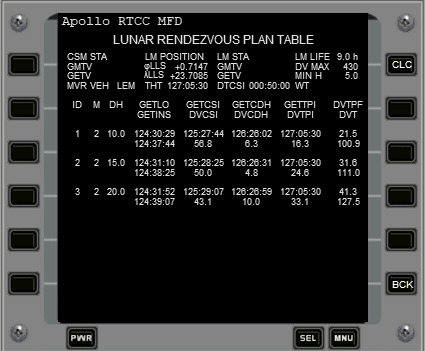
\includegraphics{./ApolloRTCCMFDFiles/RTCCMFD_LLWP_Display.png}
	\caption{Example LLWP Calculation}
	\label{fig:LLWPDisplay}
\end{figure}
\textbf{Display Parameters}\\

\textbf{CSM STA:} Station ID of CSM state vector used in the LLWP calculation.\\
\textbf{GMTV:} GMT of CSM state vector.\\
\textbf{GETV:} GET of CSM state vector.\\
\textbf{MVR VEH:} Active vehicle, performing the rendezvous maneuvers.\\
\textbf{LM POSITION:} Latitude and longitude of the lunar landing site, from which the LLWP simulates the launch.\\
\textbf{THT:} Threshold time or TPI time.\\
\textbf{LM STA:} Station ID of LM state vector used in the LLWP calculation.\\
\textbf{GMTV:} GMT of LM state vector.\\
\textbf{GETV:} GET of LM state vector.\\
\textbf{DTCSI:} Input time from insertion to CSI.\\
\textbf{LM LIFE:} LM maximum life time in hours.\\
\textbf{DV MAX:} Maximum DV of active vehicle.\\
\textbf{MIN H:} Minimum safe height for rendezvous maneuvers, in nautical miles.\\

\textbf{ID:} Number in table of solutions.\\
\textbf{M:} Number of revolutions from launch to TPI.\\
\textbf{DH:} Delta height of solution, in nautical miles.\\
\textbf{GETLO:} GET of calculated liftoff time.\\
\textbf{GETINS:} GET of calculation insertion time.\\
\textbf{GETCSI:} GET of calculated CSI time.\\
\textbf{DVCSI:} Delta V of CSI maneuver.\\
\textbf{GETCDH:} GET of calculated CDH time.\\
\textbf{DVCDH:} Delta V of CDH maneuver.\\
\textbf{GETTPI:} GET of calculated TPI time.\\
\textbf{DVTPI:} Delta V of TPI maneuver.\\
\textbf{DVTPF:} Delta V of TPF maneuver.\\
\textbf{DVT:} Total Delta V of rendezvous plan.\\

\newpage
\subsection{Deorbit Targeting}
\subsubsection{Introduction}

The retrofire targeting calculates the time of ignition and the burn parameters for a maneuver to return the spacecraft back to Earth from Low Earth Orbit. This can include a separation maneuver from the S-IVB at a fixed time before the deorbit burn. Or a shaping maneuver, that shapes the orbit before reentry, and happens at a given GET.\\

In the MFD there are pages for the definition of the separation/shaping maneuver and the retrofire maneuver respectively. To select a splashdown target and estimated time of ignition the Recovery Target Selection Display has been implemented. Finally a page to specify the type of target of the deorbit burn can be used.\\

\subsubsection{Separation/Shaping Inputs}

\textbf{SHA:} Time of ignition for the shaping maneuver. If no shaping maneuver is desired this should be set to zero.\\
\textbf{SEP:} Time in minutes that the separation maneuver will occur before the deorbit burn.\\
\textbf{THR:} Engine for the sep/shaping maneuver. Options are the SPS or the SM RCS.\\
\textbf{DV:} Fixed Delta V of the sep/shaping maneuver. Enter either a DV or a burn time, but not both.\\
\textbf{DT:} Fixed burn time of the sep/shaping maneuver. Enter either a DV or a burn time, but not both.\\
\textbf{ATT:} Attitude in LVLH coordinates of the sep/shaping maneuver. The default values are for retrograde, heads up, 31.7$^{\circ}$ window line on the horizon.\\

\textbf{UDT:} Duration of the ullage burn for the sep/shaping maneuver. Only applies to SPS maneuvers.\\
\textbf{UTH:} Number of ullage thrusters (2 or 4). Only applies to SPS maneuvers.\\
\textbf{GBL:} Calculate the gimbal angles or use system parameters. Only applies to SPS maneuvers.\\

\subsubsection{Retrofire Constraints}

\textbf{ENG:} Engine for the retrofire maneuver. Options are the SPS or the SM RCS.\\
\textbf{MOD:} Choose the burn mode for the retrofire maneuver. The options are a fixed Delta V, a fixed burn time or a maneuver to reach the reentry target line (velocity vs. flight path angle at entry interface).\\
\textbf{VAL:} Desired Delta V or burn time for the retrofire maneuver. Doesn't apply to velocity-flight path angle targeting.\\
\textbf{ATT:} Attitude mode for the retrofire maneuver. Either an input LVLH attitude or the 31.7$^{\circ}$ window line on the horizon.\\
\textbf{LVH:} LVLH attitude for the retrofire maneuver.\\
\textbf{ULL:} Ullage options for the retrofire maneuver. Only applies to the SPS.\\

\textbf{GIM:} Calculate the gimbal angles or use system parameters. Only applies to SPS maneuvers.\\
\textbf{K1:} Initial bank angle for the reentry. Held from entry interface to the specified G-Level.\\
\textbf{GC:} G-Level at which the final bank angle is started to be used.\\
\textbf{K2:} Final bank angle for the reentry. Held from the specified G-Level to drogue chute opening. In the case of target a specified latitude as well as longitude the bank angle will be reversed.\\
\textbf{BCK:} Back to deorbit targeting menu.\\

\subsubsection{Target Selection}

This program computes and displays groundtrack data for any requested 40 degrees of longitude for a requested time and starting longitude.\\

\textbf{CLC:} Calculate recovery target selection display. Inputs are a threshold time and the starting longitude.\\
\textbf{PAG:} Cycle through the pages of the display.\\
\textbf{SEL:} Choose one of the sets of coordinates on the groundtrack and save the latitude, longitude and an estimated GET for the retrofire maneuver to be used for the retrofire computation.\\
\textbf{BCK:} Back to deorbit targeting menu.\\

\subsubsection{Retrofire Calculation}

\textbf{TYP:} Choose the type of calculation. The options are type 1 (no sep/shaping maneuver) or type 2 (with sep/shaping maneuver).\\
\textbf{GET:} Estimated time of ignition for the retrofire maneuver.\\
\textbf{LAT:} Desired splashdown target latitude. Set this to a large negative value to disable targeting the latitude. The reentry profile is then a fixed bank angle and not a bank, reverse bank angle.\\
\textbf{LNG:} Desired splashdown target longitude.\\
\textbf{MD:} Maximum miss distance of the splashdown target. Can be set to a larger value to improve convergence.\\

\textbf{DIG:} Go to Retrofire Digitals display.\\
\textbf{XDV:} Go to Retrofire External DV display.\\
\textbf{SEP:} Go to Retrofire Separation display.\\
\textbf{BCK:} Back to deorbit targeting menu.\\

\newpage
\subsection{Return-to-Earth Targeting}

\subsubsection{Introduction}

The Return-to-Earth targeting calculates maneuvers for returning the spacecraft back to Earth from beyond Low Earth Orbit. For LEO maneuvers see the deorbit targeting. The objective is to calculate a single maneuver for changing the trajectory to one having safe entry-interface conditions and satisfying certain other constraints. Other constraints are dependent on the type of abort requested. The safe entry interface condition is a velocity flight path angle target line at 400,000 feet. Either of two entries maybe be specified, a shallow or a steep target line. The steep target line was used for all lunar Apollo missions.\\

Dependent upon the request, the abort maneuver will be computed considering one of three types of impact areas:

\begin{enumerate}
	\item An Unspecified Area\\
	This means that a safe reentry is guaranteed but no consideration is given to the location of the impact point (it maybe be quite undesirable).
	\item A Primary Target Point (PTP)\\
	This would be defined by a pair of latitude-longitude values. Not currently implemented in NASSP.
	\item An Alternate Target Point (ATP)\\
	This is actually not a point but is as many as five connected line segments (defined by latitude-longitude pairs) extending generally in a longitudinal direction.\\
\end{enumerate}

Both the PTP and ATP targets can be defined by manual input. The Return-to-Earth Target Table Display contains up to five PTP and five ATP target names and definitions.\\

Three general types of abort maneuvers are available.

\begin{enumerate}
	\item Time Critical Unspecified Area (TCUA)\\
	This is an inplane maneuver producing the trajectory with the earliest possible reentry. The abort is characterized by
	\begin{enumerate}
		\item Consuming all fuel provided for the maneuver, or
		\item Having the maximum allowable reentry velocity, or
		\item Having the minimum allowable time from maneuver to entry to Entry interface.
	\end{enumerate}
	\item Fuel Critical Unspecified Area (FCUA)\\
	This is an inplane maneuver requiring the least fuel to obtain a safe entry interface. Not that if the pre-abort trajectory had a safe entry interface, a request for a FCUA abort having the same target line should result in a zero DV maneuver. In practice, because of convergence tolerances, a small maneuver will be computed.
	\item ATP Abort\\
	This inplane maneuver produces a trajectory that impacts ATP trace. Multiple solutions are possible. If they exist, they are discrete and differ by twenty-four hour increments in time of landing.\\
\end{enumerate}

The abort computations are separated into three distinct steps. They are (1) the trade-off, (2) the Abort Scan Table, and (3) return-to-Earth digitals. Associated with each step in the computations is a display which summarizes the results of that step. The construction of an abort solution may be viewed as combining models of the abort maneuver, the trajectory between maneuver and entry interface, and the reentry trajectory. The three are combined in a way that will satisfy the abort criteria and the solution constraints. The trade-off, Abort Scan Table, and return-to-Earth digital computations are characterized by the models used; the models progress from less precise to more precise solutions.\\

\subsubsection{Tradeoff}

Four major questions must be answered in abort planning:
\begin{enumerate}
\item How much fuel may be expended?
\item When may the maneuver be performed?
\item How soon must splashdown occur?
\item If the target is a PTP, how large a miss is acceptable?
\end{enumerate}

There is a hidden difficulty in answering these questions — the best answer to any one of the above is not independent of the answers to the remaining three. Sometimes by relaxing tho acceptable miss by a few miles, the required velocity decreases by several thousand feet per second; sometimes shifting the time of the
maneuver by a few minutes substantially reduces the time of landing or the chance of a miss.\\
The objective of this step of the computations is to provide the user with an overall picture of the abort situation for either ATP or PTP aborts. The abort situation is defined in terms of the above four parameters (three if the target is an ATP). To this end the user supplies parameter ranges within which his solutions of interest can be found. The RTE section imposes a mesh over the solution region and examines each mesh point for a solution. Those solutions existing are used to produce analog TV displays to assist the user in arriving at an optimum answer to the four questions given above.\\
As mentioned earlier, multiple solutions having different times of landing may be available for ATP and PTP aborts. As the time of abort is varied, these times
of landing tend to vary smoothly where they exist. This leads to a natural grouping of solutions into families of solutions, each having similar times of landing.
The Tradeoff Display is a multiple page (up to five) TV display; each page contains the analog information for a different family of solutions. Two display formats are used.

\begin{enumerate}
	\item The Remote Earth ATP consisting of one analog graph, characteristic DV versus Time of Abort
	\item Near-Earth ATP consisting of three analog graphs on each page:
	\begin{enumerate}
		\item Characteristic DV versus Time of Abort\\
					One curve representing the DV required for an inplane solution that impacts the ATP trace.
		\item Time of Landing versus Time of Abort\\
					One time of landing curve corresponding to the curve in item a.
		\item Latitude of Impact versus Time of Abort\\
					One curve representing the declination of impact. Although latitude is not considered a tradeoff parameter, it is helpful to know this information.
\end{enumerate}
\end{enumerate}

The abort solutions for the Tradeoff Display are constructed by combining an impulsive velocity change, a conic (analytic two-body) trajectory, and polynomial reentry
functions. The reentry functions simulate either a high-speed G\&N entry or a constant G-level entry and are valid only if entry interface occurred on one of the
two target lines. They provide reentry range, cross range, and DT as a function of target line, entry profile and entry interface velocity, inclination, azimuth,
and latitude. Solutions constructed for the Abort Scan Table or return-to-Earth digitals will be constrained to these conic entry interface conditions.\\

Currently the tradeoff display only works in Earth reference.

\paragraph{Inputs}\mbox{} \\

\textbf{MOD:} Switch between near-Earth or remote Earth format.\\
\textbf{REM:} Choose the page (out of 5) for the remote Earth solution to be displayed\\
\textbf{SIT:} Choose the tradeoff site from the target table.\\
\textbf{TV:} Choose the vector time (MPT mode only).\\
\textbf{MIN:} Choose the minimum abort time.\\
\textbf{MAX:} Choose the maximum abort time.\\

\textbf{PAG:} Cycle between the tradeoff pages.\\
\textbf{CLC:} Calculate tradeoff solution.\\
\textbf{ENT:} Choose the entry profile.\\

\subsubsection{Abort Scan Table (AST)}

The Abort Scan Table Display is essentially a digital scratch pad that may be used to compare up to seven discrete abort solutions. One solution is inserted for
each manual AST request. These computations are more precise than the tradeoff and less precise than return-to-Earth digital computations. They consist of
an impulsive velocity change, an integrated coast trajectory, and polynomial reentry functions. The workflow to generate a Maneuver PAD or target load for a maneuver always involves first an AST calculation followed by using the Return-to-Earth Digitals.\\

Three types of AST solution can be generated. Unspecified area (time or fuel critical), specific area (ATP or PTP) and lunar search (specific site or fuel critical). The first two of these types work in both Earth and Moon sphere of influence, while the lunar search logic can only be used while in lunar orbit. The calculations that are different between Earth and Moon centered state vectors is chosen internally.\\

The two nominally used modes are lunar search for TEI and the fuel critical, unspecified area (FCUA) mode for transearth midcourse corrections.\\

\paragraph{Inputs}\mbox{} \\

\textbf{TYP:} Cycle between the three AST types.\\
\textbf{SIT:} Choose the landing site or type of abort.\\
\textbf{VTI:} Choose the vector time for the abort (MPT mode only)\\
\textbf{TIM:} Choose the time of abort, or minimum abort time in the case of lunar search.\\
\textbf{TDV:} Choose the maximum DV for a time critical abort or the maximum abort time for the lunar search option.\\
\textbf{TZ:} Choose the estimated landing time for PTP and ATP aborts.\\
\textbf{AST:} Go to the AST display page.\\
\textbf{ENT:} Choose the entry profile.\\
\textbf{MD:} Choose the maximum miss distance for a PTP abort.\\
\textbf{INC:} Choose the desired return inclination (lunar reference only). Using 0 as input will optimize the DV.\\
\textbf{BCK:} Back to entry targeting menu.\\

\paragraph{Display Buttons}\mbox{} \\
\textbf{DEL:} Delete one or all AST rows.\\
\textbf{CLC:} Calculate AST solution.\\
\textbf{RTE:} Go to RTE Digitals inputs page.\\
\textbf{BCK:} Go back to AST inputs page.\\

\paragraph{Display Explanation}\mbox{} \\

\begin{figure}[hp]
	\centering
		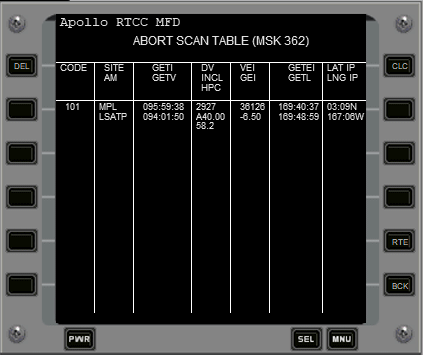
\includegraphics{./ApolloRTCCMFDFiles/Apollo11TEIASTExample.png}
	\caption{Example Abort Scan Table}
	\label{fig:Apollo11TEIASTExample}
\end{figure}

\textbf{CODE:} Code associated with the AST solution. Starts at 101 and is incremented with each new calculation.\\
\textbf{SITE:} When using PTP or ATP mode the specified landing site is shown, e.g. MPL for Mid Pacific Line.\\
\textbf{AM:} Abort Mode. First letter is E for Earth or L for Lunar centered. Second letter is S for lunar search or D for discrete time. Remaining letters show the abort type, ATP, PTP, TCUA or FCUA.\\
\textbf{GETI:} GET of the impulsive ignition.\\
\textbf{GETV:} GET of the state vector time used in the calculation.\\
\textbf{DV:} Total Delta V of the maneuver.\\
\textbf{INCL:} Earth relative inclination of the trajectory at entry interface. A for ascending and D for descending in terms of azimuth.\\
\textbf{HPC:} Height of pericynthion, only calulated in lunar reference.\\
\textbf{VEI:} Velocity at entry interface.\\
\textbf{GEI:} Flight path angle at entry interface.\\
\textbf{GETEI:} GET of entry interface.\\
\textbf{GETL:} GET of splashdown.\\
\textbf{LAT IP:} Latitude of impact.\\
\textbf{LNG IP:} Longitude of impact.\\

\subsubsection{Return-to-Earth Digitals}

The final solution produced by the RTE section — the Return-to-Earth digital solution — consists of an integrated maneuver, an integrated trajectory from the
end of the maneuver to entry interface, and an integrated reentry. Two solutions, each the result of a manual request, may be viewed with the Return-to-Earth
digital display. Either of these solutions may be transferred into the Mission Plan Table, used to initiate execution of the spacecraft setting study aid, or used to generate a command load.\\
Computation of a solution is similar to the AST computations in that the same iteration algorithm is used to adjust independent and dependent variables to meet
certain constraints on the dependent variables. The major differences can be listed:

\begin{enumerate}
	\item The first guess is a converged solution being viewed in the AST Display.
	\item The constraints at entry interface are taken from the entry interface state of the converged solution.
	\item Independent variables are the target parameters for the finite maneuver integrator (PMMRKJ).
	\item The reentry parameters are always obtained from an integrated reentry after the iteration converges to the entry interface conditions.
\end{enumerate}
The same precision trajectory logic is used by the iteration algorithm except that now the finite maneuver integrator is used to perform the maneuver instead of
making an impulsive velocity change. The user may specify to the Return-to-Earth digital computations any of four thrusters (SPS, SMRCS, DPS, or LMRCS).
In addition to requesting a solution constructed as described above, the user may manually define a solution by defining, via the manual entry device (MED) a time
for a vector fetch, a time of abort, and maneuver targets. This type of manual entry bypasses the iteration logic. The coast Encke integrator is used to propagate the fetched vector to the time of abort. The maneuver is integrated one time using the targets supplied. The coast Encke is used again to propagate the burnout vector to 400,000 feet at which point the reentry integrator is used to propagate to impact.

\paragraph{Inputs}\mbox{} \\
\textbf{COL:} Solution will be shown in either primary or manual column.\\
\textbf{AST:} Choose AST code for the calculation.\\
\textbf{REF:} Choose REFSMMAT type for the calculation. This can be any REFSMMAT currently stored in the RTCC or any of the following additional types that are calculated with the RTED solution:
\begin{itemize}
	\item ROP: Attitude is 0, 0, 0 in burn attitude with heads up. This is identical to the preferred REFSMMAT in the AGC.
	\item ROY: Attitude is 180, 180, 0 in burn attitude with heads up. This is the Earth orbit retrofire REFSMMAT.
	\item ROZ: Attitude is 0, 180, 0 in burn attitude with heads up.
	\item TEI: Attitude is 180, 0, 0 in burn attitude with heads down. This is the TEI REFSMMAT used on Apollo 12 and later.
  \item DEI: Attitude is 0, 180, 0 at reentry in an LVLH orientation with heat shield forward, inplane, lift up, heads down. This is the standard lunar entry REFSMMAT.
	\item REI: Attitude is 0, 0, 0 at reentry in an LVLH orientation with heat shield forward, inplane, lift up, heads down.
\end{itemize}
\textbf{MAN:} Choose maneuver code for the calculation. The code consists of four letters. The first letter is the spacecraft performing the maneuver, C for CSM and L for LM. The second letter is the thruster used for the maneuver. S for SPS, D for DPS or R for RCS. The third letter is the spacecraft configuration. D for docked, A for ascent stage docked and U for undocked. The last letter is always X for External DV guidance.\\
\textbf{ULL:} Choose the ullage thrusters and duration for the burn. The ullage thruster options are 2 or 4. If the burn is an RCS burn then the options are +2, +4, -2 or -4 and these will be the thrusters used for the maneuver.\\
\textbf{TRM:} Choose the trim angle option (calculated or system parameter)\\

\textbf{DIS:} Go to the RTE Digitals display\\
\textbf{DOC:} Choose the docking angle during the maneuver.\\
\textbf{HEA:} Choose heads up or down for the maneuver.\\
\textbf{ITE:} Choose iterate or not iterate for the maneuver. Iterate is the more accurate solution, but takes longer to calculate and has a small risk of not converging.\\
\textbf{BCK:} Go back to entry targeting page.\\
\paragraph{Display Buttons}\mbox{} \\

\textbf{CLC:} Calculate RTE digitals solution.\\
\textbf{SPL:} Save the splashdown target from either primary or manual column.\\
\textbf{TRA:} In non-MPT mode the TIG and DV are save to be used for uplink and Maneuver PAD. In MPT mode the maneuver gets transferred to the MPT. The input is the MED format M74. To transfer the primary column enter "M74,CSM,,RTEP;" for the manual column "M74,CSM,,RTEM;"\\
\textbf{BCK:} Go back to RTE Digitals inputs page.\\
\newpage
\paragraph{Display Explanation}\mbox{} \\

\begin{figure}[hp]
	\centering
		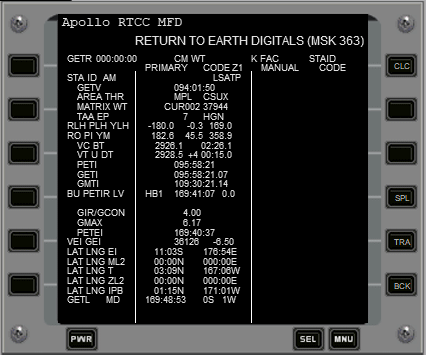
\includegraphics{./ApolloRTCCMFDFiles/Apollo11TEIRTEDExample.png}
	\caption{Example Return-to-Earth Digitals}
	\label{fig:Apollo11TEIRTEDExample}
\end{figure}

\textbf{GETR:} Reference time in GET of an event.\\
\textbf{STA ID:} Station ID of the state vector used in the calculation (MPT mode only).\\
\textbf{AM:} Abort mode, see AST display explanation.\\
\textbf{GETV:} GET of vector, see AST.\\
\textbf{AREA:} Splashdown area, see AST.\\
\textbf{THR:} Maneuver code, see RTED inputs.\\
\textbf{MATRIX:} REFSMMAT used for the calculation.\\
\textbf{WT:} Total weight at main engine on.\\
\textbf{TAA:} True anomaly after abort.\\
\textbf{EP:} Primary entry profile used to generate entry simulation. HGN for G\&N or HB1 for constant G reentry.\\
\textbf{RLH:} Roll angle at ignition in LVLH coordinates.\\ 
\textbf{PLH:} Pitch angle at ignition in LVLH coordinates.\\ 
\textbf{YLH:} Yaw angle at ignition in LVLH coordinates.\\ 
\textbf{RO:} Roll/outer gimbal angle at ignition in IMU coordinates.\\
\textbf{PI:} Pitch/inner gimbal angle at ignition in IMU coordinates.\\
\textbf{YM:} Yaw/middle gimbal angle at ignition in IMU coordinates.\\
\textbf{VC:} Delta V to be used in the EMS DV counter for the burn.\\
\textbf{BT:} Burn time of the maneuver, main engine on to cutoff.\\
\textbf{VT:} Total Delta V of the maneuver.\\
\textbf{U:} Number and direction of RCS thrusters used for ullage or as the main engines for the maneuver.\\
\textbf{DT:} Ullage duration.\\
\textbf{PETI:} Phase elapsed time of ignition, relative to GETR.\\
\textbf{GETI:} Ground elapsed time of ignition.\\
\textbf{GMTI:} GMT (since midnight launch day) of ignition.\\
\textbf{BU:} Backup entry profile.\\
\textbf{PETIR:} Phase elapsed time of initial roll (usually 0.05g)\\
\textbf{LV:} Lift vector orientation, initial roll angle.\\
\textbf{GIR/GCON:} G level of initial roll if constant G iteration was the backup entry profile. Otherwise constant G level to be used to generate backup impact coordinates.\\
\textbf{GMAX:} Maximum G level encountered during the reentry.\\
\textbf{PETEI:} Phase elapsed time of entry interface.\\
\textbf{VEI:} Velocity at entry interface.\\
\textbf{GEI:} Flight path angle at entry interface.\\  
\textbf{LAT LNG EI:} Latitude and longitude at entry interface.\\
\textbf{LAT LNG ML2:} Latitude and longitude at splashdown if primary entry mode skipped out and maximum lift was used for second entry\\
\textbf{LAT LNG T:} Latitude and longitude of the splashdown target\\
\textbf{LAT LNG ZL2} Latitude and longitude at splashdown if primary entry mode skipped out and zero lift (ballistic) was used for second entry\\
\textbf{LAT LNG IPB:} Latitude and longitude at splashdown with the backup entry mode.\\
\textbf{GETL:} GET at drogue chute deployment using the primary entry mode:\\
\textbf{MD:} Miss distance of the primary entry mode to the target splashdown coordinates. In nautical miles.\\

\newpage
\subsection{Skylab Launch Window Processor}

The launch window processor (LWP) can be used to calculate the optimal liftoff time and launch targeting parameters for Saturn IB missions to a rendezvous target in orbit, such as Skylab and ASTP. In the input descriptions below GMTLO* refers to the lift-off time that is required to achieve zero phase angle to the target at insertion.
\subsubsection{Inputs}

\textbf{PAD:} Select the launchpad (CSM or LEM). The pad coordinates are system parameters.\\
\textbf{TGT:} Select target vehicle in orbit for rendezvous. If the MPT is active then the selection is the vector time. If no vector time is given (negative value input) then either the present time is used or, if there should be any maneuvers on the MPT, the first free flight vector after the last MPT maneuver.\\
\textbf{LOT:} Liftoff time option. The options are: 

\begin{itemize}
\item{"Input time", lift-off on input time.}
\item{"Phase angle offset", compute lift-off time to achieve a desired phase angle (OFFSET) at insertion.}
\item{"Biased phase zero (GMTLOR)", lift-off on GMTLO* plus BIAS, using input time as threshold.}
\item{"Biased phase zero (TPLANE)", lift-off on GMTLO* + BIAS, using TPLANE as threshold time.}
\item{"In-plane", lift-off based on inplane launch time (GMTLO = TPLANE + TRANS).}
\item{"In-plane with nodal regression", iterate on lift-off on inplane launch time based on target orbit phase angle (final GMTLO = TYAW + TRANS).}
\end{itemize}

\textbf{CKFACT:} Chaser vehicle K-factor (drag multiplier). Not used yet.\\
\textbf{CAREA:} Chaser vehicle reference area. Not used yet.\\
\textbf{CWHT:} Chaser vehicle weight at insertion. Not used yet.\\
\textbf{NS:} Compute a launch using the northerly or southerly launch opportunity.\\
\textbf{DAY:} Day on which launch times are computed, relative to base date.\\
\textbf{PFT:} Powered flight time.\\
\textbf{PFA:} Powered flight arc.\\
\textbf{YSMAX:} Yaw steering limit.\\
\textbf{DTOPT:} Delta time to be subtracted from analytical inplane launch time to obtain empirical inplane launch time.\\
\textbf{DTGRR:} Delta time from lift-off, which defines the time of guidance reference release.\\
\textbf{RINS:} Radius of insertion in meters.\\
\textbf{VINS:} Velocity of insertion in meters per second.\\
\textbf{GAMINS:} Flight-path angle of insertion in degrees.\\
\textbf{GMTLOR:} Threshold or actual lift-off time for LOT options that require an input time.\\
\textbf{OFFSET:} Phase angle desired at insertion.\\
\textbf{BIAS:} Bias that is added to GMTLO* to produce lift-off time.\\
\textbf{TRANS:} Delta time added to inplane time to obtain lift-off time.\\
\textbf{INSCO:} Insertion cutoff conditions options:
\begin{itemize}
\item{"Input VINS, GAMINS, RINS", use the input parameters for insertion.}
\item{"Input GAMINS, RINS and height difference", calculate the insertion velocity to achieve the height difference DHW to the target at apogee after insertion.}
\item{"Input GAMINS, RINS, altitude at angle from insertion", calculate the insertion velocity to achieve the altitude DHW at the angle DU after insertion.}
\end{itemize}
\textbf{DHW:} Desired height difference between chaser and target, or altitude of chaser at input angle from insertion.\\
\textbf{DU:} Angle from insertion to obtain a given altitude or delta altitude.\\
\textbf{ANOM:} Nominal semimajor axis at insertion, used for an initial guess of the insertion velocity in the INSCO options that calculate it.\\
\textbf{DELNOF:} Flag for option to compute differential nodal regression from insertion to rendezvous.\\
\textbf{DELNO:} Angle that is added to the target descending node to account for differential nodal regression.\\
\textbf{PHASE:} Expected phase angle at insertion. The default option is 90-270$^{\circ}$, which should work for most of the 0-360$^{\circ}$ range. Near 360$^{\circ}$ some difficulty to converge could arise, so if a calculation fails then switching this option to 270-540$^{\circ}$ can help. Other than that there should be no need to change the default value.\\
\textbf{LAZCOE:} Coefficients of the empirical launch azimuth polynomial. The polynomial has the form \(A\textsubscript{z} = A\textsubscript{00} + A\textsubscript{01}i + A\textsubscript{10}\lambda + A\textsubscript{11}i\lambda\), where i is the inclination and \(\lambda\) is the descending node angle. All input and output angles in radian. \\
\textbf{DIS:} Go to launch targeting display.\\ 
\textbf{BCK:} Go back to utilities page.\\

\newpage
\subsubsection{Display}

\begin{figure}[hp]
	\centering
		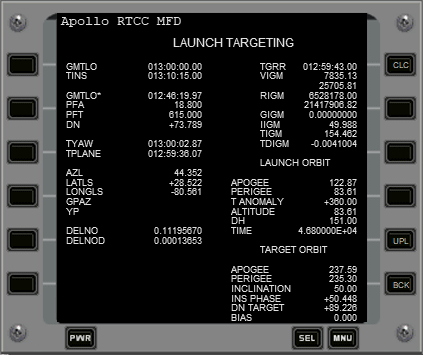
\includegraphics{./ApolloRTCCMFDFiles/LaunchTargetingDisplay.png}
	\caption{Launch Targeting Display for Skylab 2}
	\label{fig:LaunchTargetingDisplayExample1}
\end{figure}

\textbf{GMTLO:} Greenwich mean time of lift-off, in hours, minutes, seconds\\
\textbf{TINS:} Greenwich mean time of insertion, in hours, minutes, seconds\\
\textbf{GMTLO*:} Greenwich mean time of phase match, in hours, minutes, seconds\\
\textbf{PFA:} Powered flight arc.\\
\textbf{PFT:} Powered flight time.\\
\textbf{DN:} Descending node of chaser.\\
\textbf{TPLANE:} Greenwich mean time of inplane launch, in hours, minutes, seconds\\
\textbf{AZL:} Optimum launch azimuth.\\
\textbf{LATLS:} Geocentric latitude of launch site.\\
\textbf{LONGLS:} Geographic longitude of launch site.\\
\textbf{DELNO:} Angle between the target and chaser descending nodes, defined at insertion.\\
\textbf{DELNOD:} Rate of change of DELNO, defined at insertion.\\
\textbf{TYAW:} Greenwich mean time of lift-off to achieve minimum yaw steering, in hours, minutes, seconds\\
\textbf{TGRR:} Greenwich mean time of guidance reference release\\
\textbf{VIGM:} Velocity magnitude at insertion, in meters per second and feet per second.\\
\textbf{RIGM:} Radius magnitude at insertion, in meters and feet\\
\textbf{GIGM:} Flightpath angle at insertion\\
\textbf{IIGM:} Inclination at insertion\\
\textbf{TIGM:} Angle measured from launch site meridian to chaser descending node, defined at TGRR\\
\textbf{TDIGM:} Rate of change of TIGM, defined at TGRR\\
\textbf{APOGEE:} Height of apogee in nautical miles\\
\textbf{PERIGEE:} Height of perigee in nautical miles\\
\textbf{INCLINATION:} Inclination of orbit plane\\
\textbf{INS PHASE:} Phase angle at insertion\\
\textbf{DN TARGET:} Descending node of target\\
\textbf{BIAS:} Time added to GMTLO* time to obtain a lift-off time\\
\textbf{T ANOMALY:} True anomaly\\
\textbf{ALTITUDE:} Height of chaser at, insertion\\
\textbf{DH:} Delta height between chaser and target, at insertion\\
\textbf{TIME:} Greenwich mean time of lift-off\\

\newpage
\section{Pre-Advisory Data}
\subsection{Maneuver PAD}

\subsubsection{Explanation}

The Maneuver Pre-Advisory Data (PAD) contains all necessary numbers to safely conduct a burn with the SPS or RCS. A complete explanation of each item on the PAD can be found in all Apollo flight plans, e.g. \href{http://history.nasa.gov/alsj/a11/a11fltpln_final_reformat.pdf}{here}. Additionally to the Maneuver PAD the very similar Apollo 7 TPI PAD was added as a second mode.\\ 

\subsubsection{Buttons}

\textbf{VEH:} Cycle between using the docked (CSM/LM) or undocked vehicle configuration for the maneuver.\\
\textbf{ENG:} Cycle between the available thrusters for the maneuver.\\
\textbf{HEA:} Choose between conducting the maneuver in a heads-up or a heads-down orientation.\\
\textbf{ULL:} Choose the ullage thrusters (2 or 4) and ullage duration for the maneuver.\\
\textbf{TIG:} If you want to display a Maneuver PAD for a maneuver not calculated with the Apollo RTCC MFD you can manually enter the desired Time of Ignition and Delta V.\\
\textbf{DV:} See above.\\
\textbf{CLC:} Calculate the Maneuver PAD.\\
\textbf{OPT:} Switch between the CSM and LM Maneuver PADs, the Apollo 7 TPI PAD, the TLI PAD and the PDI PAD.\\
\textbf{STA:} Choose the time before the maneuver for which the sextant star check, boresight star check and backup GDC alignment are calculated.\\
\textbf{GDC:} Choose the preferred star set for the backup GDC alignment. There are four sets of stars that can be used for the alignment. The Maneuver PAD logic will usually first try Deneb and Vega and perform an occultation check and a yaw angle check (75 deg max.). If this set is not available it will attempt to use the next one. With this button the preferred set, which will be checked first, can be selected. If it is not available the PAD would still show a different set that is available. The time for which the checks are performed is the same time as selected for the sextant and boresight star check.\\
\textbf{BCK:} Go back to the main menu.\\
\newpage
\subsection{Entry PAD}

\subsubsection{Explanation}

The Entry PAD contains all numbers to conduct a safe reentry. There are two types of Entry PADs: Earth Orbit Reentry and Lunar Entry. A complete explanation of each item on the PAD can be found in most Apollo flight plans, e.g. \href{http://history.nasa.gov/alsj/a11/a11fltpln_final_reformat.pdf}{here}. \\

\subsubsection{Buttons}

\textbf{MAN:} For a lunar entry you can choose between calculating a direct Entry PAD without any additional maneuvers or a Entry PAD for a previously calculated Midcourse Correction. For an Earth orbit entry a deorbit maneuver has to be performed in any case.\\
\textbf{DWN:} Downlink the splashdown coordinates from the AGC.\\
\textbf{CLC:} Calculate the missing numbers on the Entry PAD.\\
\textbf{OPT:} Switch between the Earth Entry PAD and the Lunar Entry PAD.\\
\textbf{BCK:} Go back to the main menu.\\
\newpage
\subsection{Landmark Tracking}

\subsubsection{Explanation}

On the Landmark Tracking page coordinates on the spherical bodies (Earth and Moon) in Orbiter 2010 can be converted to AGC coordinates. Also the contents of a Landmark Tracking PAD can be calculated. These are used for the correct timing of a pitchdown maneuver for better tracking with Program 22.

T1 is the time at which the CSM comes over the horizon and becomes visible from the landmark. At this time the astronaut can begin looking at the landmark to find the specific point he wants to track. \\
T2 is the time at which the CSM is at an elevation angle of 35$^{\circ}$ from the landmark. If any marks on the landmark are to be done, then at this time the pitchdown maneuver should be started. In Earth orbit this is usually 0.5$^{\circ}$/s, in lunar orbit 0.3$^{\circ}$/s. \\
The other displayed values are the distance of the landmark from the ground track of the CSM orbit and the AGC inputs. The AGC uses geodetic latitude, longitude divided by 2 and altitude in nautical miles as the inputs.\\

\subsubsection{Buttons}

\textbf{TIM:} Estimated time over the landmark.\\
\textbf{LAT:} Geocentric latitude of the landmark.  If the landmark is listed in a marker file, then that latitude should be used as an input here.\\
\textbf{LNG:} Longitude of the landmark.\\
\textbf{CLC:} Calculate AGC coordinates and Landmark Tracking PAD.\\
\newpage
\subsection{Map Update}

\subsubsection{Explanation}

The Map Update is very different in Earth and Moon orbit. In Earth orbit the next ground station with the times of acqusition and loss of signal (AOS and LOS) are displayed.  In lunar orbit a few more times are displayed: loss of signal (LOS), sunrise (SR), crossing of the prime meridian (PM), acqusition of signal (AOS) and sunset (SS) are shown. These values are written down on the Apollo 8 Map Update forms.\\ 

\subsubsection{Buttons}

\textbf{CLC:} Calculate map update.\\
\textbf{MOD:} Cycle between Earth and Moon orbit.\\
\newpage
\subsection{AGS State Vector Update}
\subsubsection{Explanation}
This page shows the AGS State Vector Update PAD. There would also be a MOCR display for the same function (MSK 277) but this page has been modelled after the PAD given to the crew for covenience. The AGS SV PAD can be used to manually input CSM and LM state vectors on the DEDA. This is a backup method, the main method of updating the state vectors would be via downlink from the PGNS (Verb 47).\\
Because the AEA uses no REFSMMAT the coordinate system of the state vectors depends on the current alignment being used. For that the current REFSMMAT in use can be selected. The RTCC keeps several REFSMMAT stored, the main ones for this page would be the current (CUR) or AGS REFSMMATs. As the PGNS and AGS typically use the same alignment the CUR REFSMMAT would be saved as the AGS REFSMMAT and then the AGS REFSMMSAT is used for the state vector calculation. But any REFSMMAT in the LM REFSMMAT table can be used.\\
This page can also be used to manually or automatically update the AGS K-Factor. For the automatic option the current PGNS and AGS clocks are compared and the difference is then saved as the K-Factor.\\
\subsubsection{Buttons}
\textbf{SLT:} Cycle between updating the CSM or the LM part of the PAD.\\
\textbf{TGT:} Update the CSM or LM vessel.\\
\textbf{REF:} Choose the REFSMMAT in the LM REFSMMAT table to use for the state vector calculation.\\
\textbf{AGS:} Manually enter the AGS K-Factor.\\
\textbf{KFA:} Run the automatic calculation to update the K-Factor.\\
\textbf{CLC:} Calculate the AGS state vector PAD. CSM and LM state vectors are calculated separately.\\
\textbf{SAV:} Save the present LM CUR REFSMMAT as the AGS REFSMMAT. All REFSMMATs in the LM REFSMMAT table can be used for the state vector calculation, but only the AGS REFSMMAT is used in converting telemetry vectors (see Vector Panel Summary) so this is a simple way to update the AGS REFSMMAT. The alternative would be using the G00 MED.\\
\newpage
\section{Utilities}
\subsection{REFSMMAT}
\subsubsection{Explanation}

The REFSMMAT (REFerence to Stable Member MATrix) is a rotation matrix relating the Apollo Basic Reference Coordinate System (BRCS) and the currently used IMU Stable Member Coordinate System. Depending on the mission phase the REFSMMAT is chosen, so that the IMU angles provide meaningful attitude values. Some types of REFSMMATs can be calculated by the AGC itself, but most were uplinked to the spacecraft from the ground. The REFSMMATs that can be calculated with this MFD are:

\begin{itemize}
	\item{Launch: Calculates the Launch REFSMMAT, which is also calculated internally in the AGC at liftoff.}
	\item{Landing Site: Not used for Apollo 7 or 8}
	\item{PTC: Passive Thermal Control, not used for Apollo 7 or 8.}
	\item{LOI-2: A special LVLH REFSMMAT for Apollo 8, calculated before the last translunar Midcourse Correction.}
	\item{P30: Alignment for a thrusting maneuver, equivalent to option 1 in Program 52.}
	\item{P30 retro: Alignment for a retrograde burn, useful for Earth orbit reentry maneuvers.}
	\item{LVLH: Local Vertical alignment, equivalent to option 2 in Program 52.}
	\item{Lunar Entry: Equivalent to option 2 in Program 52 with the GET of Entry Interface.}
\end{itemize}
	
\subsubsection{Buttons}
	\textbf{TIM:} The options "Landing Site"', "PTC", "`P30", "P30 retro " and "LVLH" require a time in GET to calculate the REFSMMAT. For a Landing Site REFSMMAT the time chosen is either the predicted landing or launch time. The time for P30 and P30 retro REFSMMATs is the maneuver time and is set on a maneuver calculation page (Lambert, CDH or Entry).\\
	\textbf{TYP:} Choose betwen uplinking the REFSMMAT or the desired REFSMMAT. The desired REFSMMAT is the alignment, that Program 52 will align the platform to, based on the knowledge of the attitude referenced to the old, currently used REFSMMAT. Only in rare cases the REFSMMAT itself would be uploaded, e.g. when activating the Lunar Module or if the difference to the previous REFSMMAT is very small. In doubt, uplink the desired REFSMMAT!\\
	\textbf{DWN:} Downlink the current REFSMMAT from the AGC. If the type of REFSMMAT is known, select it by cycling through the REFSMMAT types by pressing OPT before doing the downlink. Useful for calculating PADs with a REFSMMAT not calculated by the RTCC MFD.\\
	\textbf{MCC:} The calculated REFSMMAT usually depends heavily on the current orbit. If there is a maneuver between now and the set time or the reentry time, change the setting to MCC to take the maneuver into account. The LOI-2 REFSMMAT is special, because the calculation of two maneuver is required before the LOI-2 REFSMMAT can be calculated. This will be explained in more detail on the Lunar Insertion page.\\
	\textbf{OPT:} Switch between the different options.\\
	\textbf{CLC:} Calculate the REFSMMAT.\\
	\textbf{UPL:} Uplink the REFSMMAT to the AGC.\\
	\textbf{LAT:} Only for Landing Site: Choose the latitude of the landing site.\\
	\textbf{LNG:} Only for Landing Site: Choose the longitude of the landing site.\\
	\textbf{BCK:} Go back to the main menu.\\
	\subsection{Apollo Generalized Optics Program}

The Apollo Generalized Optics Program (AGOP) contains various optics and antenna pointing calculations.\\

Option 1 of the AGOP will be used for cislunar navigation. This program option defines an inertial attitude which will align the optics system to the horizon or some specified landmark on the Earth or Moon. Output consists of IMU gimbal angles and the optics shaft and trunnion angles to point the sextant at the specified star.\\

Option 2 will accept a state vector and compute the right ascension and declination of the spacecraft with respect to the Earth, and the right ascension and declination of the Earth, Moon and Sun with respect to the Earth. Additionally it computes the same quantities referenced to an input landmark when mode 2 is selected. Mode 2 will compute right ascension, declination, and a unit vector from the spacecraft to the specified landmark or the center of the Earth, Moon and Sun as desired\\

Option 3 will output the right ascension, declination and unit vector of all stars in the catalog.\\

Option 4 will accept a state vector and IMU gimbal angles and compute the pitch and yaw angles of the onboard S-Band Hi-Gain Antenna, S-Band Steerable Antenna, and Rendezvous Radar Antenna necessary to point at a specified ground based radar. An additional option provides the capability of fixing the antenna position and computing the necessary spacecraft gimbal angles for pointing the antenna at a specified ground station.\\

Option 5 computes the IMU gimbal angles required to place the spacecraft in a passive thermal control (PTC) attitude, with the +X-axis oriented 90 degrees with respect to the Sun and to the Earth for omnidirectional communication.\\

Option 6 computes the attitude required to orientate the CSM to the forward or aft horizons, either in heads up or down.\\

Option 7 (Optics Support Table) will primarily be used to verify the CMC and LGC stable member alignment made by using the onboard optical sighting equipment. This option is divided into 5 modes which are as follows:\\

Mode 1 computes the yaw angle required to place the LM z-axis in the local vertical plane and a pitch angle which will place the horizon on the landing point designator LPD). The necessary inputs are REFSMMAT, gimbal angles, and time.\\

Mode 2 uses an input REFSMMAT, spacecraft attitude, and time interval to compute AOS, LOS, and optics angles for 10 stars.\\

Mode 3 computes a REFSMMAT by specifying star IDs, optics angles, and spacecraft attitude. The capability exists to input two sets of gimbal angles with the above input data and compute the REFSMMAT.\\

Mode 4 uses an input REFSMMAT and spacecraft attitude for both vehicles to compute the second vehicle REFSMMAT. If both REFSMMATs are input, the second vehicle attitude will be computed.\\

Mode 5 computes the CSM gimbal angles required to point the AOT at the desired target. The inputs are REFSMMAT, docking angle, one star ID, and optics angles.\\

Mode 6 computes the attitude for the preferred REFSMMAT. Given a current and a desired REFSMMAT, it computes the gimbal angles for the current REFSMMAT, which define 0, 0, 0 gimbal angles for the preferred REFSMMAT and outputs a set of gimbal angles and FDAI angles which used in conjuction with the current REFSMMAT defines the spacecraft attitude necessary to switch to the preferred REFSMMAT and read 0, 0, 0 gimbal angles.\\

Options 8 and 9 will be implemented in the future.\\
\newpage
\subsection{VECPOINT}

\subsubsection{Explanation}

The VECPOINT page, named after a routine in the AGC, is calculating the IMU angles to point a specific part of the CSM or LM in the direction of a celestial object/astronomical body. Any body present in Orbiter 2010 can be chosen. The X-axis of the spacecraft is along its longitudinal axis, so +X is pointing the CSM directly at the body and the SPS engine directly away from it.\\

\subsubsection{Buttons}

\textbf{BOD:} Type the name of the body e.g. Sun, Moon etc.\\
\textbf{DIR:} Choose the direction of the spacecraft to be pointed at the celestial object.\\
\textbf{CLC:} Calculate the IMU angles.\\
\newpage
\subsection{S-IVB Lunar Impact Targeting}
The Lunar Targeting Program (LUNTAR) was a software available at the Marshall Space Flight Center to calculate the burns of the S-IVB Auxiliary Propulsion System (APS) to cause the S-IVB to impact the Moon in a desired place (Apollo 13 and later). The S-IVB performed a short APS burn and a LOX dump shortly after the CSM/LM separated from it which caused the S-IVB to be on an impact trajectory, but not yet to the desired coordinates. There were usually two midcourse corrections scheduled for the S-IVB, the first one being non-zero.\\

The targeting available in the RTCC MFD has three different modes. First a Trajectory Evaluation mode which checks where (if at all) the S-IVB will impact the Moon without any further APS burn. Then a Burn Evaluation mode which shows the impact coordinates given an input APS burn. And lastly the actual targeting mode which calculates the required burn to reach the required coordinates. The desired coordinates and the initial guess for the APS MCC-1 can be found in lunar impact postflight evaluation reports which can be found on NTRS, e.g. this one for \href{https://ntrs.nasa.gov/citations/19710002523}{Apollo 13}. \\

The uplink to the IU for the impact targeting can currently not be done in the RTCC MFD, but in the Project Apollo MFD instead. This might be moved in the future.\\

\subsubsection{Inputs}
\textbf{MOD:} Cycle between the three calculation modes described above.\\
\textbf{TIG:} Enter the time of ignition in Ground Elapsed Time.\\
\textbf{BT:} Enter the estimated burn time in seconds.\\
\textbf{PIT:} Enter the estimated LVLH pitch attitude of the maneuver in degrees.\\
\textbf{YAW:} Enter the estimated LVLH yaw attitude of the maneuver in degrees.\\
\textbf{LAT:} Enter the desired lunar impact latitude in degrees.\\
\textbf{LNG:} Enter the desired lunar impact longitude in degrees.\\
\textbf{OPT:} Either optimize the Delta V of the burn or enforce a specific lunar impact time.\\
\textbf{IMP:} Enter the desired lunar impact time in Ground Elapsed Time.\\

\subsubsection{Outputs}
\begin{itemize}
	\item Time of ignition referenced to the start of Timebase 8
	\item Calculated (or input) burn time
	\item Calculated (or input) LVLH pitch angle in degrees
	\item Calculated (or input) LVLH yaw angle in degrees
	\item Actual lunar impact latitude in degrees
	\item Actual lunar impact longitude in degrees
	\item Actual lunar impact flight-path angle in degrees
\end{itemize}

\newpage
\subsection{Powered Descent Abort Program}
\subsubsection{Explanation}
The Powered Descent Abort Program (PDAP) calculates the parameters used by the PGNS and AGS during an abort from powered descent, to guide the LM to a trajectory that will lead to rendezvous with the CSM using the normal coelliptic rendezvous sequence. For the nominal PDI attempt (PDI-1) these parameters have already been loaded in the LGC and AEA during prelaunch and were rarely updated during the mission. If a second PDI attempt (PDI-2) has to be performed an update of the descent abort constants is required for a good rendezvous with the CSM.\\

The onboard computer calculations using the abort constants generate a horizontal velocity to be achieved by orbit insertion after the abort. The scheme to calculate this velocity, and the parameters used in its calculation, differed from mission to mission.\\

In the Apollo 11 PGNS the calculation involves a polynomial of the horizontal velocity as a function of time of abort initiation. Due to differing performance between APS and DPS two polynomials are used. One set for the case that the abort is initiated using the DPS engine (P70), the other set for the case the abort is initiated with the ascent stage directly (P71).\\

In the Apollo 11 AGS (using the Flight Program 6 software) the horizontal velocity is calculated from the desired insertion semi-major axis, which is a linear function of phase angle to the CSM. This eliminates most differences between APS only vs. DPS+APS aborts so only one set of parameters has to be loaded.\\

The Apollo 12 PGNS software switched to using the AGS calculation scheme with one important addition. A late powered descent abort would require a very low insertion orbit. Because typically a lower limit for the apolune altitude of 30 NM was enforced the rendezvous profile for a late abort would require an additional maneuver. The updated PGNS software instead added a second phase of descent aborts that would achieve rendezvous with the CSM one orbit later with a slightly different rendezvous profile. So the set of abort constants now consisted of the two parameters for a linear function, then a limiting phase angle at which the guidance switches to the second abort segment, and lastly the two parameters for the second linear function.\\

The AGS software also switched to using this two segment scheme, but the next version of the AGS software was not ready until Apollo 13. This is the reason why the PDAP in the RTCC MFD has three versions selectable by mission number, with Apollo 12 flying a PGNS software that has two segments, but an AGS software (using the same general calculation scheme) only having one segment. A late powered descent abort using the AGS would have required some special procedures.\\

One other thing to note is that later Apollo missions performed DOI with the CSM and the CSM also performed a circularization maneuver before PDI. These maneuvers change the relative trajectory between CSM and LM. In some cases the first powered descent abort segment now actually had the rendezvous with the CSM one orbit later than the second segment, which is the reverse order from Apollo 12. A table with suggested inputs for all the abort variants used on the Apollo missions is provided to clarify the differences between missions.\\
\subsubsection{Inputs}
\textbf{MIS:} Selection for the PGNS and AGS software versions. The three options are Apollo 11, 12 and 13+.\\
\textbf{ENG:} Selelect the engine for the abort. Either the abort is started immediately using the ascent stage (APS engine) or the abort is started using the DPS, with staging potentially happening later when the DPS runs out of propellant (see WTDRY below). For the Apollo 11 PGNS both cases are run automatically.\\
\textbf{CSM:} Select the CSM vehicle name or the CSM vector if the Mission Plan Table feature is enabled.\\
\textbf{LM:} Select the LM vehicle name or the LM vector if the Mission Plan Table feature is enabled. The weight of this vehicle (or at the selected time) will be used as the initial weight at PDI.\\
\textbf{HAMIN:} Select the minimum apolune altitude in nautical miles. This altitude is used as the segment switch or end of calculations for the descent aborts.\\
\textbf{DH:} Select the delta height at the CDH maneuver during the coelliptic rendezvous that follows the descent abort.\\
\textbf{K4:} Some of the later Apollo missions start powered descent at a fairly high phase angle (read distance) to the CSM. Some aborts on these trajectories would not run into the apolune limit (HAMIN) but would have the first onboard calculated rendezvous maneuver (CSI) at such a high range from the CSM that very little onboard navigation (Rendezvous Radar or VHF ranging) could be done before the maneuver has to be performed. For these cases an alternative segment switch point has been implemented. This flag switches between either using the apolune altitude HAMIN as the segment switch point or a phase angle at abort (PHA input) that represents a limit on the range to the CSM. Using the phase angle option the first segment of an abort would have the TPI maneuver one orbit later so that the CSI maneuver also happens later and closer to the CSM. Once the CSM is closer to the LM at abort initiation the rendezvous profile with TPI happening one orbit earlier is then possible. The second segment of a descent abort always ends at the apolune limit HAMIN.\\
\textbf{PHA:} The limiting phase angle at abort initiation that is used to limit the range to the CSM at the first onboard calculated maneuver (CSI). See K4 for a detailed explanation.\\
\textbf{DTCAN:} Delta time between orbit insertion and the canned maneuver. The canned maneuver is a maneuver with a fixed Delta V that is included in some rendezvous profiles. It is usually called the boost maneuver in the flight data files.\\
\textbf{DVCAN:} LVLH components of the canned maneuver.\\
\textbf{DTCSI:} Delta time between the canned maneuver and CSI.\\
\textbf{TTPI:} TPI time used to generate the first set of targeting coefficients. This time can be calculated with the TPI times page using the 16 minutes before sunrise option.\\
\textbf{DT2CAN:} Value of DTCAN used to generate the second set of targeting coefficients.\\
\textbf{DV2CAN:} Value of DVCAN used to generate the second set of targeting coefficients.\\
\textbf{DT2CSI:} Value of DTCSI used to generate the second set of targeting coefficients.\\
\textbf{T2TPI:} Value of TTPI used to generate the second set of targeting coefficients.\\
\textbf{WTDRY:} LM weight representative of DPS fuel depletion. Leave the input blank to automatically calculate this value (present LM weight minus DPS propellant).\\
\textbf{WTAPS:} LM weight immediately after staging. Leave the input blank to automatically calculate this value (present LM ascent stage weight).\\
\subsubsection{Suggested Inputs}
\begin{tabular}{|m{2.0cm}|m{1.85cm}|m{1.85cm}|m{1.85cm}|m{1.85cm}|m{1.85cm}|}
  \hline
  \textbf{Input}&\textbf{Apollo 11 PDI-1/2}&\textbf{Apollo 12 PDI-1/2}&\textbf{A13-15 PDI-1/2}&\textbf{A16/17 PDI-1}&\textbf{A16/17 PDI-2}\\
	\hline
  \textbf{MIS}&11&12&13+&13+&13+\\
	\hline
  \textbf{ENG}&-&DPS/APS&DPS/APS&DPS/APS&DPS/APS\\
	\hline
	\textbf{K4}&-&HAMIN*&PHA$\dagger$&PHA$\dagger$&PHA$\dagger$\\
	\hline
	\textbf{PHA}&-&-&-13.5&16.0&-13.5\\
  \hline
	\textbf{DTCAN}&0&0&60&0&60\\
	\hline
	\textbf{DVCAN}&0 0 0&0 0 0&10 0 0&0 0 0&10 0 0\\
  \hline
	\textbf{DTCSI}&50&50&120&55&120\\
	\hline
	\textbf{TTPI}&PDI+2:40&PDI+2:40&PDI+4:50&PDI+2:50&PDI+4:50\\
	\hline
  \textbf{DT2CAN}&-&50&0&50&0\\
	\hline
  \textbf{DV2CAN}&-&10 0 0&0 0 0&10 0 0&0 0 0\\
  \hline
	\textbf{DT2CSI}&-&110&55&110&55\\
	\hline
	\textbf{T2TPI}&-&PDI+4:40&PDI+2:50&PDI+4:50&PDI+2:50\\
	\hline
\end{tabular}

\hfill

*HAMIN = First segment apolune limit\\
$\dagger$PHA = First segment phase angle limit\\
\newpage
\subsubsection{Display}
\paragraph{Apollo 11 PGNS}\mbox{} \\
\textbf{DPS4-1} P70 polynomial. Horizontal insertion velocity as a function of abort initiation time since PDI.\\
\textbf{APS4-1} P71 polynomial. Horizontal insertion velocity as a function of abort initiation time since PDI.\\
\textbf{VHMIN} Minimum horizontal insertion velocity.
\paragraph{Apollo 12+ PGNS}\mbox{} \\
\textbf{J1} Constant value in first segment calculation of insertion semi-major axis.\\
\textbf{K1} Slope value in first segment calculation of insertion semi-major axis.\\
\textbf{J2} Constant value in second segment calculation of insertion semi-major axis.\\
\textbf{K2} Slope value in second segment calculation of insertion semi-major axis.\\
\textbf{THET} Limiting phase angle at abort initiation for the segment switch.\\
\textbf{VHMIN} Minimum horizontal insertion velocity.
\paragraph{Apollo 11-12 AGS}\mbox{} \\
\textbf{J7} Constant value in calculation of insertion semi-major axis. DEDA address 224.\\
\textbf{J8} Minimum insertion semi-major axis. DEDA address 225.\\
\textbf{J9} Maximum insertion semi-major axis. DEDA address 226.\\
\textbf{K410} Slope value in calculation of insertion semi-major axis. DEDA address 227.
\paragraph{Apollo 13+ AGS}\mbox{} \\
\textbf{J7} Constant value in first segment calculation of insertion semi-major axis. DEDA address 224.\\
\textbf{J8} Minimum insertion semi-major axis. DEDA address 225.\\
\textbf{J10} Constant value in second segment calculation of insertion semi-major axis. DEDA address 226.\\
\textbf{J12} Limiting phase angle at abort initiation for the segment switch. DEDA address 305.\\
\textbf{K410} Slope value in first segment calculation of insertion semi-major axis. DEDA address 662.\\
\textbf{J11} Slope value in first segment calculation of insertion semi-major axis. DEDA address 673.\\
\newpage
\section{Uplinks}

\subsection{State Vector}

\subsubsection{Explanation}

The state vector of the vessel can be calculated and uplinked here. Additionally to the functionality in the Project Apollo MFD, this MFD can calculate a state vector in the future, which sometimes was used during the Apollo program to prevent an internal state vector integration of the AGC.\\
The AGC has two slots for state vectors: CSM and LM. For the CSM the MFD will prevent uplinking a state vector that is not the vessel itself. The vessel for the LM can be freely chosen.\\

\subsubsection{Buttons}

\textbf{MOD:} Choose  between calculating the state vector "now" and at a specified GET.\\
\textbf{TIM:} Set the desired GET for the state vector in GET mode.\\
\textbf{TGT:} Set the target vessel.\\
\textbf{SLT:} Switch between the slots.\\
\textbf{CLC:} Calculate a state vector.\\
\textbf{UPL:} Uplinks the calculated data to the AGC.\\
\textbf{BCK:} Go back to the main menu.\\

\section{Mission Planning}

The mission plan table (MPT) is the central planning tool in the RTCC for future maneuvers. The RTCC has two MPTs, one for the CSM and one for the LM, which are related through undocking and docking maneuvers. Each MPT consists of a table header and data blocks for each individual maneuver. The table header has the initial vehicle configuration (combinations of CSM, Saturn and LM ascent and/or descent stages) and initial weights, area (for drag calculations) and propellant. Each maneuver block has data describing the maneuver and updates weights and propellant.\\

At the current stage of RTCC development for NASSP the MPT is an optional feature that can be used to plan and evaluate future maneuvers. The RTCC MFD has a MPT mode which by default is off. When it is switched on then current state vectors and weights are not updated automatically but have to be managed manually. However, the MPT header is already used in the non-MPT mode for trajectory propagation for state vector uplinks. In the future more parts of the MFD will use the data in the MPT header.\\

There are four manual user entry (MED) modes to update the MPT header. The M55 MED is used to establish the initial vehicle configuration, time to start S-IVB venting and the initial CSM/LM docking angle. M51 is used to update the vehicle areas and a K-factor (multiplier) for drag calculations. In MPT mode the M50 MED is used to update vehicle weights and M49 is used to update available propellants. The detailed MED inputs and format can be found in the MED section of the manual.\\
\subsection{MPT Initialization}

On the left side of this page appear the input parameters that are automatically or manually updated. On the right side the page shows the actual data stored in the MPT.\\

\subsubsection{Buttons}
\textbf{TAB:} Choose the mission plan table (CSM or LM) to initialize.\\
\textbf{MED:} Choose the type of initialization to do. The options are M49 for propellants, M50 for weights, M51 for vehicle areas or M55 for the initial vehicle configuration.\\
\textbf{UPD:} To update the MPT (right side) with the data currently set as input (left side).\\
\textbf{$<<$:} Go to previous item to manually change input data.\\
\textbf{$>>$:} Go to next item to manually change input data.\\
\textbf{SET:} Change the currently selected input.\\
\textbf{TGT:} Select a vessel in the simulation to automatically populate the input data.\\
\textbf{AUT:} Automatically update the input data with the selected vessel.\\
\textbf{VPS:} Go to the Vector Panel Summary page for MPT state vector management.\\
\textbf{BCK:} Go back to the main menu.\\
\newpage
\section{Example: Apollo 7 Rendezvous}

This MFD can be used to replicate the ground solutions for the rendezvous and other SPS burns during the Apollo 7 mission. As an example the inputs for the following maneuvers will be presented:

\begin{enumerate}
	\item {NCC1 burn at 26:25:00 GET.}
	\item {NCC2 burn at 27:30:00 GET.}
	\item {NSR burn at 28:01:00 GET.}
	\item {TPI burn at ca. 29:25:00 GET.}
\end{enumerate}

\subsection{NCC1 burn}

At 26:25:00 GET a SPS burn was executed that will put the CSM on a trajectory resulting in a phase angle of 1.32$^{\circ}$ behind and 8NM below the SIVB at 28:00:00GET. The maneuver is calculated with the Two-Impulse Multiple Solution display. The required inputs are:

\begin{itemize}
  \item{VEH is set to CSM.}
	\item{Both maneuver times are fixed (IV option)}
	\item{The Chaser vessel is AS-205, the target vessel is AS-205-S4BSTG.}
	\item{T1 is set to 26:25:00 GET (NCC1 time).}
	\item{T2 is set to 28:01:00 GET (NSR time).}
	\item{The desired offsets are 8.0 NM for DEL H, 1.32 deg for PHASE, 27.45 deg for ELEV (at TPI) and 140 deg for WT (travel angle from TPI to TPF)} 
\end{itemize}

On the TI Multiple Solution display only this one maneuver will appear. With the TRA button the maneuver can be converted to a finite burn, taking the maneuver engine into account (SPS). The resulting burn solution should be close to the vector (+62.7, -1.0, +154.8). This can be used in a P30/P40 automatic SPS burn with the CSM.

%\subsection{NCC2 burn}

%This is essentially a midcourse correction burn to remove any deviations from the desired trajectory. All parameters used in the NCC1 stay the same, with two exceptions. The maneuver time T1 has a GET of 27:30:00. The number of revolutions from NCC2 to NSR also is now clearly 0, instead of 1.\\
%If the NCC1 burn was accurate, then this will result in a very low DV. During testing it never exceeded 2 feet per second.

\subsection{NSR burn}

The NSR burn nominally happens at 28:00:00 GET and places the CSM in a coelliptic orbit with a constant delta height to the target. On the CDH page of the MFD the inputs for the burn are the GET (028:00:00) and the Delta Height (DH) of the orbit, which is 8 NM for Apollo 7. Because the GET is variable, the option "Find GETI" should be used. A positive value here means below the target. When calculating the burn, the new time for the maneuver is also displayed below the number for DH. The new time is chosen, so that the delta height of the burn is exactly the specified 8NM. The results should be close to:

\begin{itemize}
	\item{028:00:30 GET}
	\item{DX: -92.7 fps}
	\item{DY: +1.6 fps}
	\item{DZ: -106.2 fps}
\end{itemize}

These numbers can be used for the external DV program (P30).

\subsection{TPI burn}

The TPI maneuver nominally was calculated by the AGC itself, but a backup solution was calculated on the ground. This backup solution can be replicated with the MFD.\\
On the Two Impulse Multiple Solution page first set the S-IVB as the target. Then press T1 and enter any negative number. The MFD will now try to find the T1, when an elevation angle of 27.45$^{\circ}$ occurs, provided this angle has been entered using the P51 button. To find the T2 time, which is 140 degrees of orbital travel after T1, press T2 and enter a negative time again. T2 will now be calculated in the TI processor. Usual values for the maneuver:

\begin{itemize}
	\item{29:21:38 GET}
	\item{DX: +13.7 fps}
	\item{DY: +0.9 fps}
	\item{DZ: -7.9 fps}
\end{itemize}
	
On the Maneuver PAD page press OPT and CLC to display the TPI PAD.\\

%\section{Example: Apollo 8}

%\subsection{LOI-2 REFSMMAT}

%The REFSMMAT for the Lunar Orbit Circulation (LOI-2) REFSMMAT "is such that if a horizontal, in-plane, heads-up, posigrade burn were being made at LOI-2, the gimbal angle (FDAI) readout would be approximately 0,0,0. (R-P-Y)."\\

%To achieve these conditions calculate a preliminary LOI-1 burn with IMFD or LTMFD and receive the numbers for the burn with Project Apollo MFD. If you have the time of ignition and the Delta V components, open the Apollo RTCC MFD and set these numbers on the Maneuver PAD page via the manual TIG and DV inputs. Now go back to the main menu and select the REFSMMAT page and choose LVLH as the REFSMMAT option. The required time will be set to the TIG of the LOI-2 maneuver, which is 73:30:54 GET. Press CLC and uplink the solution. \\
\newpage
\section{Example: Midcourse Correction Planning}
\subsection{Example 1: Apollo 11 MCC-2}

As mentioned in the introduction of this section, the version of the midcourse correction processor implemented in the RTCC MFD was used for Apollo 14 to 17. Apollo 11 would have used mode 2 of the processor for their MCC-2. Modes 2 and 4 were changed to only apply to the LOI/DOI maneuver sequence of those later missions. The same capability was retained in modes 3 and 5 though, by inputting the same desired azimuth as min and max azimuth on the constraints page.\\

To start off the calculation, go to the SFP page, under Maneuver Targeting, Translunar, Skeleton Flight Plan Table. The SFP contains initial guesses and some targeting parameters that the MCC calculation requires. The premission data is stored in tables that are valid for the whole daily launch window, so the first step is to the select the data set for the actual launch conditions. Press the F62 button and check that the first TLI opportunity and the correct launch azimuth usually 72 deg) are entered. After pressing enter the MFD page should now be populated with data. This step has to be done just once per mission and otherwise no changes will have to be done on the SFP page.\\

The next step happens under Maneuver Targeting, Translunar, Midcourse Processor. This takes you to the computation page of the processor. Here choose mode 3 (click twice on the MAN button). The Apollo 11 MCC-2 happened at about 26:45:00 GET, so press the TIG button and input that time. The other inputs can be left as they are. The solution will be shown in column 1, the maneuver is docked and the skeleton flight plan table no. 1 contains the preflight estimates. Press CON to check that all the constraints are as desired, especially the min and max azimuth constraints being identical. This should already be preloaded in the MFD, so no changes are necessary.\\ Back to the previous page (BCK button) and then to the midcourse tradeoff display (MID button) and everything should be ready for the calculation. Press CLC and the solution for the mode 3 calculation should be displayed in column 1. Using the Apollo 11 Before MCC-2 scenario that comes with NASSP this results in a maneuver of 19.7 ft/s (DV MCC).\\

You can now try different inputs and constraints, but if you are happy with the solution, you should now save the resulting data table from the MCC-2 calculation for use in the later MCC-3 and MCC-4 calculations. That is done by pressing the F30 button and typing: \emph{F30,1;} The result can be checked under MCC Display, MSK button, "1597" input, F31 button. The F31 cycles between the preflight (table 1) and the nominal (table 2) targets. Only table 2 will be saved in scenarios.\\

Back to the Midcourse Tradeoff page, the maneuver still has to be converted from an impulsive, instant maneuver to a finite maneuver taking the thruster being used into account. For that click on the MPT button and then on the THR button until the thruster of your choice is selected. SPS is set by default and is the correct choice for the maneuver. Click the CLC button and the actual TIG and DV have now been generated. These can be used to display e.g. a Maneuver PAD for the midcourse.\\

\subsection{Example 2: Apollo 11 MCC-4}

MCC-4 will use the nodal targets (latitude, longitude, radius and time of the desired position at LOI, if it was an instant velocity change maneuver) that resulted from the MCC-2 calculation, and were stored in skeleton flight plan table number 2. MCC-4 is a mode 1 maneuver with a time of ignition of about 70:55:00 GET. Input this value with the TIG button, then press the SFP button so that it says 2, for SFP table 2. Go to the midcourse tradeoff display and press CLC. Converting it to a finite maneuver works the same way as for MCC-2. Possibly MCC-4 will be small enough to be done with the RCS.\\

\subsection{Example 3: Apollo 12 MCC-2}

Apollo 12 was the first mission to fly the so called hybrid mission profile. After TLI the trajectory is ideally free return, but with a pericynthion altitude higher than necessary for successful lunar orbit insertion. Therefore there has to be a midcourse correction that takes the trajectory to a close encounter with the Moon, but in the process making it non-free return. This maneuver was planned for MCC-2. After MCC-2 the same LOI-1 and LOI-2 maneuvers were flown as on the previous missions.\\

To accomplish the hybrid transfer maneuver, mode 5 of the midcourse processor has to be used. Use a TIG of about 30:53h GET, column 1, docked vehicle configuration and table 1 (preflight targets) of the skeleton flight plan. Use the MID button to go to the midcourse tradeoff display and then press CLC to calculate the solution. It should now have calculated fairly large maneuver, the nominal Delta V being 68.8 ft/s.\\

The trajectory after MCC-2 is not constrained to be free return, but was instead optimized for the smallest possible Delta V. This will also potentially have moved the time of ignition for LOI-1 away from the flight plan time. If it is not critical that the DV optimal solution for MCC-2 is being used, the LOI-1 TIG can be adjusted by constraining that time on the constraints page. This was done on the actual Apollo 12 mission and is not possible for free-return missions like Apollo 11.\\

The flight plan time for LOI-1 is 83:25:18.2 GET. Check which time ("GET LOI") the midcourse tradeoff page is showing after calculating the MCC-2 solution. If the times are different by more than a few seconds go to the midcourse constraints page and press the F23 button. The times that are input here are not directly the LOI GET, but instead the pericynthion time, which is a bit later than LOI-1. The convergence of the constrained solution works best if the minimum and maximum times input with the F23 button are 10 minutes apart. Usually the LOI TIG will now run into the lower or upper end of the constraint. As you can't predict on which end of the time window LOI will now be, this process is always one of trial and error. So start by inputting a min and max time that contains the GET of LOI. Then recalculate the solution on the midcourse tradeoff page and check what the new LOI GET is. By moving the time window to later or earlier times with the F23 button the LOI GET can be moved as well. This might take a few iterations until the LOI GET is close to the desired time. A few seconds off are acceptable\\

After this solution resulting in the desired LOI-1 time has been calculated the process is the same as for the Apollo 11 MCC-2. After committing to performing the maneuver as calculated use the F30 button to store the data table containing the numbers required to calculate MCC-3 and MCC-4. These are calculated with mode 1 just like for Apollo 11.\\

\subsection{Example 4: Apollo 13 MCC-2}

\newpage
\section{Example: Deorbit Targeting}
\subsection{Example 1: Apollo 11 Pre TLI Abort}

Should the mission be aborted at the earliest time after reaching orbit, the first deorbit opportunity is the Atlantic ocean area, just one orbit after launch.

The CSM/S-IVB separation procedure used in computing this reentry is a 5-second SM RCS burn in the retrograde horizon monitor attitude. The separation is begun 20 minutes prior to the deorbit burn and places the CSM below and behind the S-IVB at retrofire. The horizon monitor attitude mentioned here is the nominal deorbit attitude and is attained by aligning a mark on the CM window with the earth horizon.\\

From the circular 100 NM orbit the velocity vs. flight path angle targeting for entry interface cannot be used, as there would be too little time between cutoff of the retrofire maneuver and reentry. Therefore a fixed Delta V of 325 ft/s is used, which leads to a slightly shallow reentry, but enough time for the procedures before reentry.\\

To start setting up for this calculation, review the MFD page with the inputs for the separation maneuver. The page is located under Maneuver Targeting, Deorbit, Separation/Shaping Constraints. The default values for all inputs are set up for this type of separation maneuver. The LVLH pitch angle corresponds to placing the window mark on the horizon from a 100 NM orbit. So nothing has to be changed on this page.\\

Next go to the Retrofire Constraints page. Here only the retrofire mode has to be changed from "V, Gamma" to "DV". Then enter a DV of 325 ft/s with the VAL button. The other constraints should be correctly set up. SPS engine, 31.7 deg window line, 4 quads, 15 seconds ullage, CUR REFSMMAT, compute gimbal angles. For the reentry the initial bank angle of 0 deg will be held, followed at 0.2g by a bank angle of 55 deg.\\

Next the splashdown target is selected on the Target Selection Display. Go to that page, press CLC and enter "1:0:0 -70" for a threshold GET of 1h and the desired splashdown longitude of 70 deg west. The display will now show groundtrack data, starting at that longitude. The time at that longitude should be about 1:40h GET. Now press the SEL button to select the first set of data (at 70 deg west). This will automatically generate the target for the retrofire maneuver.\\

Now go to the Retrofire Maneuver page. The estimated TIG, latitude and longitude are filled in from the target selection before. The type of maneuver has to be changed to type 2, to include the separation maneuver. Miss distance can be left at 1 NM. Now go to the main output display for the calculation, the Retrofire Digitals, with the DIG button. There the maneuver can be calculated with the CLC button.\\

\subsection{Example 2: Apollo 9 nominal deorbit}

The procedure to calculate a nominal deorbit maneuver is very similar to the one described in the previous example. Instead of the fixed Delta V of 325 ft/s the V, gamma target line is used. The calculation is of type 1 (no sep/shaping maneuver), so none of the inputs on the MFD page for the sep/shaping maneuver apply. The splashdown longitude is 59.9 deg west.\\

\subsection{Example 3: Skylab deorbit}

The Skylab missions performed the deorbit in two steps. First a SPS burn called the shaping maneuver, which lowers the perigee to 90 NM. Then, about two orbits later, the actual deorbit maneuver, again with the SPS, was done.\\

The easiest method to target this maneuver sequence is, contrary to the naming, use of the separation burn logic, so that the two maneuvers are separated by a specific time difference. Here the common inputs for the shaping and deorbit maneuver:\\

\textbf{Definition of Separation/Shaping Maneuver (R30)}\\
\textbf{SHA}: No Shaping Maneuver\\
\textbf{SEP}: 180 min (initial guess for two full orbits between the two maneuvers)\\
\textbf{THR}: SPS\\
\textbf{DV}: 250 ft/s (initial guess from Skylab orbital altitude)\\
\textbf{DT}: 0.0 s\\
\textbf{ATT}: 180.0 -15.0 180.0 (pitched down 15 degrees from local horizontal, heads down)\\
\textbf{UDT}: 20.0\\
\textbf{UTH}: 2 jet ullage\\
\textbf{GBL}: Compute Gimbal Trims\\

\textbf{Retrofire Constraints (R31)}\\
\textbf{ENG}: SPS\\
\textbf{MOD}: V, Gamma\\
\textbf{VAL}: N/A\\
\textbf{ATT}: LVLH\\
\textbf{LVH}: 180.0 -15.0 180.0 (pitched down 15 degrees from local horizontal, heads down)\\
\textbf{ULL}: 2 quads, 20 seconds\\
\textbf{MAT}: DES (desired orientation, gives the IMU attitude 0, 180, 0 in burn attitude)\\
\textbf{GIM}: Compute Gimbal Trims\\
\textbf{K1}: 0.0 deg\\
\textbf{GC}: 0.2 gs\\
\textbf{K2}: 55.0 deg\\

\textbf{Retrofire Planning (R32)}\\
\textbf{TYP}: Type 2 (With Sep/Shaping)\\

Select the target point like in example 1. Two input values have to be tweaked manually with trial and error to get a satisfying solution. First, the Delta V of the shaping maneuver is a manual input, so it has to be changed until the perigee altitude after the maneuver is 90 NM. This value, as well as the other burn parameters of the shaping burn, can be found on the Retrofire Separation (MSK 355) display. In a second step, to optimize the Delta V of the deorbit burn, the time difference from shaping to deorbit has to be adjusted. This is the SEP button on the "Definition of Separation/Shaping Maneuver" page. The deorbit burn should occur near apogee, so tweak this input value until a minimum Delta V of the deorbit burn is reached.\\

\newpage
%\renewcommand{\arraystretch}{2}
\begin{landscape}
\section{Manual Entry Device (MED) Formats}

\subsection{Acronyms}

\begin{itemize}
	\item \textbf{EBCDIC}: \href{https://en.wikipedia.org/wiki/EBCDIC}{Extended Binary Coded Decimal Interchange Code} (Characters)\\
	\item \textbf{FLP}: Floating Point\\
	\item \textbf{FXP}: Fixed Point (Integer)\\
	\item \textbf{MSK}: Manual Select Keyboard (display number)\\
\end{itemize}
\newpage

\subsection{MED List}

\textbf{MED Code}: C10\\
\textbf{Purpose}: Initiate a CMC/LGC external delta-v update\\
\textbf{Example}: \texttt{C10,CMC,1,CSM;}

\begin{center}
\begin{tabular}{|c|*{6}{>{\centering\arraybackslash}m{2.1cm}|} }
 \hline
 \diagbox{\textbf{Desc.}}{\textbf{Item}} & \textbf{1} & \textbf{2} & \textbf{3} & \textbf{4} & \textbf{5} & \textbf{6} \\ 
 \hline
 \textbf{Item Name} &Vehicle Type&Maneuver Number&MPT Indicator&&&\\
 \hline
 \textbf{Input Format} &EBCDIC&FXP&EBCDIC&&& \\
 \hline
 \textbf{Input Units} &&&&&& \\
 \hline
 \textbf{Checking Option}&Exact&Min/Max(2)&Exact(3)&&&\\
 \hline
 \textbf{Missing Item Option}&Error(1)&Error&Error&&&\\
 \hline
\end{tabular}
\end{center}

\begin{tabbing}
\textbf{Notes}:\= (1) CMC, LGC\\
\> (2) 1-15\\
\> (3) CSM/LEM\\
\end{tabbing}
\newpage

\textbf{MED Code}: G00\\
\textbf{Purpose}: CSM/LM REFSMMAT locker movement\\
\textbf{Example}: \texttt{G00,LEM,LLD,CSM,CUR;}

\begin{center}
\begin{tabular}{|c|*{6}{>{\centering\arraybackslash}m{2.1cm}|} }
 \hline
 \diagbox{\textbf{Desc.}}{\textbf{Item}} & \textbf{1} & \textbf{2} & \textbf{3} & \textbf{4} & \textbf{5} & \textbf{6} \\ 
 \hline
 \textbf{Item Name} &CSM/LEM Vehicle&Matrix 1&CSM/LEM Vehicle&Matrix 2&GET&\\
 \hline
 \textbf{Input Format} &XXX&XXX&XXX&XXX&XXX:XX:XX& \\
 \hline
 \textbf{Input Units} &EBCDIC&EBCDIC&EBCDIC&EBCDIC&HH:MM:SS& \\
 \hline
 \textbf{Checking Option}&Exact&Exact&Exact&Exact&$^{\leq}$0Current Time&\\
 \hline
 \textbf{Missing Item Option}&Error&Error&Error&Error&=Current Time&\\
 \hline
\end{tabular}
\end{center}

\textbf{Notes}: For matrix 1, valid codes are CUR, PCR, TLM, OST, MED, DMT, DOK, LCV, DOD, LLA, LLD, AGS for the LEM and CUR, PCR, TLM, OST, MED, DMT, DOD, LCV for the CSM. For matrix 2, valud codes are CUR, PCR, TLM, MED and LCV for the CSM and CUR, PCR, TLM, MED, LCV, LLA, and AGS for the LEM.\\
\newpage

\textbf{MED Code}: G03\\
\textbf{Purpose}: Compute and save local vertical CSM/LM platform alignment\\
\textbf{Example}: \texttt{G03,CSM,100:00:00;}

\begin{center}
\begin{tabular}{|c|*{6}{>{\centering\arraybackslash}m{2.1cm}|} }
 \hline
 \diagbox{\textbf{Desc.}}{\textbf{Item}} & \textbf{1} & \textbf{2} & \textbf{3} & \textbf{4} & \textbf{5} & \textbf{6} \\ 
 \hline
 \textbf{Item Name} & CSM or LEM Vehicle & GET &&&&\\
 \hline
 \textbf{Input Format} &XXX&XXX:XX:XX&&&& \\
 \hline
 \textbf{Input Units} &EBCDIC&HH:MM:SS&&&& \\
 \hline
 \textbf{Checking Option}&Exact&&&&&\\
 \hline
 \textbf{Missing Item Option}&Error&Error&&&&\\
 \hline
\end{tabular}
\end{center}

\begin{tabbing}
\textbf{Notes}:
\end{tabbing}
\newpage

\textbf{MED Code}: M10\\
\textbf{Purpose}: CSM and LM thrust characteristics\\
\textbf{Example}: \texttt{M10,S,,1,20000,20673,65.62;}

\begin{center}
\begin{tabular}{|c|*{6}{>{\centering\arraybackslash}m{2.1cm}|} }
 \hline
 \diagbox{\textbf{Desc.}}{\textbf{Item}} & \textbf{1} & \textbf{2} & \textbf{3} & \textbf{4} & \textbf{5} & \textbf{6} \\ 
 \hline
 \textbf{Item Name} &Thruster Code&Total no. of entries in table&Entry no. of this set&Weight&Thrust Level&Weight Loss Rate\\
 \hline
 \textbf{Input Format} &EBCDIC&FXP&FXP&FLP&FLP&FLP \\
 \hline
 \textbf{Input Units} &S, A, D&&&lbs&lbf&lbs\\
 \hline
 \textbf{Checking Option}&&1$\leq$X$\leq$40&1$\leq$X$\leq$40&X$\geq$1000&0$\leq$X$\leq$28000&\\
 \hline
 \textbf{Missing Item Option}&Error&Ignore&Error&Error&Error&Error\\
 \hline
\end{tabular}
\end{center}

\begin{tabbing}
\textbf{Notes}:
\end{tabbing}

\newpage

\textbf{MED Code}: M11\\
\textbf{Purpose}: CSM and LM CG characteristics\\
\textbf{Example}: \texttt{M11,C,,1,20000,1.0,2.0,3.0;}

\begin{center}
\begin{tabular}{|c|*{6}{>{\centering\arraybackslash}m{2.1cm}|} }
 \hline
 \diagbox{\textbf{Desc.}}{\textbf{Item}} & \textbf{1} & \textbf{2} & \textbf{3} & \textbf{4} & \textbf{5} & \textbf{6} \\ 
 \hline
 \textbf{Item Name} &Vehicle&Total no. of entries in table&Entry no. of this set&Weight&X coordinate of CG&Y coordinate of CG\\
 \hline
 \textbf{Input Format} &EBCDIC&FXP&FXP&FLP&FLP&FLP \\
 \hline
 \textbf{Input Units} &C, L, A&&&lbs&inches&inches\\
 \hline
 \textbf{Checking Option}&&1$\leq$X$\leq$40&1$\leq$X$\leq$40&&&\\
 \hline
 \textbf{Missing Item Option}&Error&Ignore&Error&Error&Error&Error\\
 \hline
\end{tabular}
\end{center}

\begin{tabbing}
\textbf{Notes}:
\end{tabbing}
\newpage
\textbf{MED Code}: M11 (cont.)\\
\textbf{Purpose}: \\
\textbf{Example}: \\

\begin{center}
\begin{tabular}{|c|*{6}{>{\centering\arraybackslash}m{2.1cm}|} }
 \hline
 \diagbox{\textbf{Desc.}}{\textbf{Item}} & \textbf{1} & \textbf{2} & \textbf{3} & \textbf{4} & \textbf{5} & \textbf{6} \\ 
 \hline
 \textbf{Item Name} &Z coordinate of CG&&&&&\\
 \hline
 \textbf{Input Format} &FLP&&&&& \\
 \hline
 \textbf{Input Units} &inches&&&&& \\
 \hline
 \textbf{Checking Option}&&&&&&\\
 \hline
 \textbf{Missing Item Option}&Error&&&&&\\
 \hline
\end{tabular}
\end{center}

\begin{tabbing}
\textbf{Notes}:
\end{tabbing}

\newpage
\textbf{MED Code}: M49\\
\textbf{Purpose}: Change fuel remaining weights\\
\textbf{Example}: \texttt{M49,CSM,20000;}

\begin{center}
\begin{tabular}{|c|*{6}{>{\centering\arraybackslash}m{2.1cm}|} }
 \hline
 \diagbox{\textbf{Desc.}}{\textbf{Item}} & \textbf{1} & \textbf{2} & \textbf{3} & \textbf{4} & \textbf{5} & \textbf{6} \\ 
 \hline
 \textbf{Item Name} &MPT Code&SPS Fuel Remaining&CSM RCS Fuel Remaining&S-IVB J-2 Remaining&APS Fuel Remaining&LM RCS Fuel Remaining\\
 \hline
 \textbf{Input Format} &EBCDIC&FLP&FLP&FLP&FLP&FLP \\
 \hline
 \textbf{Input Units} &CSM, LEM&lbs.&lbs.&lbs.&lbs.&lbs. \\
 \hline
 \textbf{Checking Option}&&$\geq$0&$\geq$0&$\geq$0&$\geq$0&$\geq$0\\
 \hline
 \textbf{Missing Item Option}&Error&Insert neg. number&Insert neg. number&Insert neg. number&Insert neg. number&Insert neg. number\\
 \hline
\end{tabular}
\end{center}

\begin{tabbing}
\textbf{Notes}: A change of fuel will \underline{not} cause a trajectory update.
\end{tabbing}
\newpage

\textbf{MED Code}: M49 (cont.)\\
\textbf{Purpose}: \\
\textbf{Example}: \\

\begin{center}
\begin{tabular}{|c|*{6}{>{\centering\arraybackslash}m{2.1cm}|} }
 \hline
 \diagbox{\textbf{Desc.}}{\textbf{Item}} & \textbf{1} & \textbf{2} & \textbf{3} & \textbf{4} & \textbf{5} & \textbf{6} \\ 
 \hline
 \textbf{Item Name} &DPS Fuel Remaining&&&&&\\
 \hline
 \textbf{Input Format} &FLP&&&&& \\
 \hline
 \textbf{Input Units} &lbs.&&&&& \\
 \hline
 \textbf{Checking Option}&$\geq$0&&&&&\\
 \hline
 \textbf{Missing Item Option}&Insert neg. number&&&&&\\
 \hline
\end{tabular}
\end{center}

\begin{tabbing}
\textbf{Notes}:
\end{tabbing}
\newpage

\textbf{MED Code}: M50\\
\textbf{Purpose}: Change vehicle weights\\
\textbf{Example}: \texttt{M50,CSM,40000;}

\begin{center}
\begin{tabular}{|c|*{6}{>{\centering\arraybackslash}m{2.1cm}|} }
 \hline
 \diagbox{\textbf{Desc.}}{\textbf{Item}} & \textbf{1} & \textbf{2} & \textbf{3} & \textbf{4} & \textbf{5} & \textbf{6} \\ 
 \hline
 \textbf{Item Name} &MPT Code&CSM Weight&S-IVB Weight&LM Total Weight&LM Ascent Weight&Time of Weight\\
 \hline
 \textbf{Input Format} &EBCDIC&FLP&FLP&FLP&FLP&HH:MM:SS\\
 \hline
 \textbf{Input Units} &CSM, LEM&lbs.&lbs.&lbs.&lbs.&lbs. \\
 \hline
 \textbf{Checking Option}&&$\geq$2000&$\geq$2000&$\geq$2000&$\geq$2000&$\leq$Present Time\\
 \hline
 \textbf{Missing Item Option}&Error&Insert neg. number&Insert neg. number&Insert neg. number&Insert neg. number&Insert neg. number\\
 \hline
\end{tabular}
\end{center}

\begin{tabbing}
\textbf{Notes}:
\end{tabbing}
\newpage

\textbf{MED Code}: M51\\
\textbf{Purpose}: Change vehicle cross-sectional area or K-factor\\
\textbf{Example}: \texttt{M51,CSM,129.4;}

\begin{center}
\begin{tabular}{|c|*{6}{>{\centering\arraybackslash}m{2.1cm}|} }
 \hline
 \diagbox{\textbf{Desc.}}{\textbf{Item}} & \textbf{1} & \textbf{2} & \textbf{3} & \textbf{4} & \textbf{5} & \textbf{6} \\ 
 \hline
 \textbf{Item Name} &MPT Code&CSM Area&S-IVB Area&LM Ascent Area&LM Descent Area&K-Factor\\
 \hline
 \textbf{Input Format} &EBCDIC&FLP&FLP&FLP&FLP&FLP\\
 \hline
 \textbf{Input Units} &CSM, LEM&ft.\textsuperscript{2}&ft.\textsuperscript{2}&ft.\textsuperscript{2}&ft.\textsuperscript{2}&ft.\textsuperscript{2}\\
 \hline
 \textbf{Checking Option}&&$0\leq$X$\leq$2000&$0\leq$X$\leq$2000&$0\leq$X$\leq$2000&$0\leq$X$\leq$2000&$-30\leq$X$\leq$30\\
 \hline
 \textbf{Missing Item Option}&Error&Insert neg. number&Insert neg. number&Insert neg. number&Insert neg. number&Insert neg. number\\
 \hline
\end{tabular}
\end{center}

\begin{tabbing}
\textbf{Notes}:
\end{tabbing}
\newpage

\textbf{MED Code}: M55\\
\textbf{Purpose}: Input initialization parameters\\
\textbf{Example}: \texttt{M55,CSM,CSL;}

\begin{center}
\begin{tabular}{|c|*{6}{>{\centering\arraybackslash}m{2.1cm}|} }
 \hline
 \diagbox{\textbf{Desc.}}{\textbf{Item}} & \textbf{1} & \textbf{2} & \textbf{3} & \textbf{4} & \textbf{5} & \textbf{6} \\ 
 \hline
 \textbf{Item Name} &MPT Code&Configuration Code&GET to begin venting&Delta Docking Angle&&\\
 \hline
 \textbf{Input Format} &EBCDIC&EBCDIC&HH:MM:SS&FLP&&\\
 \hline
 \textbf{Input Units} &CSM, LEM&Note 1&GET&degrees&&\\
 \hline
 \textbf{Checking Option}&Exact&Exact&&&&\\
 \hline
 \textbf{Missing Item Option}&Error&Insert "FF"&Insert neg. number&Insert "FF"&&\\
 \hline
\end{tabular}
\end{center}

\begin{tabbing}
\textbf{Notes}: Note 1: Any combination of C (CSM), S (SIVB), L (LEM: Ascent+Descent), A (LEM: Ascent Only), D (LEM: Descent Only)
\end{tabbing}
\newpage

\textbf{MED Code}: P08\\
\textbf{Purpose}: Update pitch angle from horizon\\
\textbf{Example}: \texttt{P08,31.6;}

\begin{center}
\begin{tabular}{|c|*{6}{>{\centering\arraybackslash}m{2.1cm}|} }
 \hline
 \diagbox{\textbf{Desc.}}{\textbf{Item}} & \textbf{1} & \textbf{2} & \textbf{3} & \textbf{4} & \textbf{5} & \textbf{6} \\ 
 \hline
 \textbf{Item Name} &Pitch Angle&&&&&\\
 \hline
 \textbf{Input Format} &FLP&&&&& \\
 \hline
 \textbf{Input Units} &degrees&&&&& \\
 \hline
 \textbf{Checking Option}&None&&&&&\\
 \hline
 \textbf{Missing Item Option}&Error&&&&&\\
 \hline
\end{tabular}
\end{center}

\begin{tabbing}
\textbf{Notes}:
\end{tabbing}
\newpage

\textbf{MED Code}: P10\\
\textbf{Purpose}: Update liftoff time for specified vehicle\\
\textbf{Example}: \texttt{P10,CSM,13:32:00;}

\begin{center}
\begin{tabular}{|c|*{6}{>{\centering\arraybackslash}m{2.1cm}|} }
 \hline
 \diagbox{\textbf{Desc.}}{\textbf{Item}} & \textbf{1} & \textbf{2} & \textbf{3} & \textbf{4} & \textbf{5} & \textbf{6} \\ 
 \hline
 \textbf{Item Name} &Vehicle&GMTALO&Traj/No traj Ind.&&&\\
 \hline
 \textbf{Input Format} &EBCDIC&H:M:S(.TH)&EBCDIC&&& \\
 \hline
 \textbf{Input Units} &VEH&hours&EBCDIC&&& \\
 \hline
 \textbf{Checking Option}&Note 1&T$\geq$0.&Exact (note 4)&&&\\
 \hline
 \textbf{Missing Item Option}&Error&Error&Insert "NO TRAJ"&&&\\
 \hline
\end{tabular}
\end{center}

\begin{tabbing}
\textbf{Notes}:\= (1) Veh. must be in MHGVNM (CSM, LEM)\\
\> (2): First veh. (MGLGMT, MCGMTL), second veh. (MGGGMT, MCGMTS)\\
\> (3): Must be "TRAJ" or "NO TRAJ" ("TRAJ" allowed in NPHASE, PRELAUNCH, PRELAUNCH 2 (L.S.))\\
\end{tabbing}
\newpage

\textbf{MED Code}: P12\\
\textbf{Purpose}: Enter GMTGRR and launch azimuth for selected vehicle\\
\textbf{Example}: \texttt{P12,CSM,13:32:00,72.0;}

\begin{center}
\begin{tabular}{|c|*{6}{>{\centering\arraybackslash}m{2.1cm}|} }
 \hline
 \diagbox{\textbf{Desc.}}{\textbf{Item}} & \textbf{1} & \textbf{2} & \textbf{3} & \textbf{4} & \textbf{5} & \textbf{6} \\ 
 \hline
 \textbf{Item Name} &Vehicle&GMTGRR&Launch Azimuth&&&\\
 \hline
 \textbf{Input Format} &EBCDIC&H:M:S(.TH)&FLP&&& \\
 \hline
 \textbf{Input Units} &EBCDIC&hours&deg.&&& \\
 \hline
 \textbf{Checking Option}&Exact 1&$\geq$0&70.$\leq$A$\leq$110.&&&\\
 \hline
 \textbf{Missing Item Option}&Error&Error&Error&&&\\
 \hline
\end{tabular}
\end{center}

\begin{tabbing}
\textbf{Notes}: \= (1) CSM, IU1, IU2. IU1 and IU2 valid at all times. CSM valid only prior to GOST initialization.\\
\> (2) See GMSMED documentation (flowchart).
\end{tabbing}
\newpage

\textbf{MED Code}: P13\\
\textbf{Purpose}: Enter vector in spherical coordinates\\
\textbf{Example}: \texttt{P13,CSM,5521.0,0.0,269.0,0.7,23.4,60.0,102:40:00,L,MCT;}

\begin{center}
\begin{tabular}{|c|*{6}{>{\centering\arraybackslash}m{2.1cm}|} }
 \hline
 \diagbox{\textbf{Desc.}}{\textbf{Item}} & \textbf{1} & \textbf{2} & \textbf{3} & \textbf{4} & \textbf{5} & \textbf{6} \\ 
 \hline
 \textbf{Item Name} &Vehicle&Velocity&Flight Path Angle&Azimuth&Geocentric Latitude&Longitude\\
 \hline
 \textbf{Input Format} &EBCDIC&FLP&FLP&FLP&FLP&FLP\\
 \hline
 \textbf{Input Units} &EBCDIC&ft./sec.&degrees&degrees&degrees&degrees\\
 \hline
 \textbf{Checking Option}&Note 1&$\geq$0&-90.$\leq$A$\leq$90&0.$\leq$A$\leq$360&-90.$\leq$A$\leq$90&-180.$\leq$A$\leq$180\\
 \hline
 \textbf{Missing Item Option}&Error&&&&&\\
 \hline
\end{tabular}
\end{center}

\begin{tabbing}
\textbf{Notes}: \= (1) Vehicle must be in vehicle name table (CSM, LEM)\\
\end{tabbing}
\newpage

\textbf{MED Code}: P13\\
\textbf{Purpose}: Enter vector in spherical coordinates\\
\textbf{Example}: \texttt{P13,CSM,5521.0,0.0,269.0,0.7,23.4,60.0,102:40:00,L,MCT;}

\begin{center}
\begin{tabular}{|c|*{6}{>{\centering\arraybackslash}m{2.1cm}|} }
 \hline
 \diagbox{\textbf{Desc.}}{\textbf{Item}} & \textbf{7} & \textbf{8} & \textbf{9} & \textbf{10} &&\\ 
 \hline
 \textbf{Item Name} &Height&Time&Live/Static Ephem. Ind.&Coordinate System Ind.&&\\
 \hline
 \textbf{Input Format} &FLP&H:M:S.TH&EBCDIC&EBCDIC&&\\
 \hline
 \textbf{Input Units} &NM&hours&EBCDIC&EBCDIC&&\\
 \hline
 \textbf{Checking Option}&H$\geq$0&T$\geq$0&Exact Note 2&Exact Note 3&&\\
 \hline
 \textbf{Missing Item Option}&&&Insert L&Insert ECT&&\\
 \hline
\end{tabular}
\end{center}

\begin{tabbing}
\textbf{Notes}: \= (2) \= Possible inputs:\\
\> \>-L - Live ephem. (default)\\
\> \>-B = put in GZLTRA and STATIC ephem.\\
\> \>-S = STATIC ephem.\\
\> \>-G = Put in GZLTRA only.\\
\> (3) Coord. System Ind. = ECT, MCT\\
\end{tabbing}
\newpage

\textbf{MED Code}: P15\\
\textbf{Purpose}: Update GMTZS for specified vehicle\\
\textbf{Example}: \texttt{P15,AGC,13:32:00;}

\begin{center}
\begin{tabular}{|c|*{6}{>{\centering\arraybackslash}m{2.1cm}|} }
 \hline
 \diagbox{\textbf{Desc.}}{\textbf{Item}} & \textbf{1} & \textbf{2} & \textbf{3} & \textbf{4} & \textbf{5} & \textbf{6} \\ 
 \hline
 \textbf{Item Name} &Vehicle&GMTZS&DT from GMTZS (LGC) to AGS on&&&\\
 \hline
 \textbf{Input Format} &EBCDIC&hours&hours&&& \\
 \hline
 \textbf{Input Units} &EBCDIC&hours&hours&&& \\
 \hline
 \textbf{Checking Option}&Exact 1&$\geq$0&$\geq$0&&&\\
 \hline
 \textbf{Missing Item Option}&Error&Ignore&Ignore&&&\\
 \hline
\end{tabular}
\end{center}

\begin{tabbing}
\textbf{Notes}: \= (1) AGC, LGC, AGS\\
\> (2) See Flowchart of GMSMED for storing details.\\
\end{tabbing}
\newpage

\textbf{MED Code}: P16\\
\textbf{Purpose}: Generate an ephemeris for one vehicle using a vector from the other vehicle\\
\textbf{Example}: \texttt{P16,CSM,LEM;}

\begin{center}
\begin{tabular}{|c|*{6}{>{\centering\arraybackslash}m{2.1cm}|} }
 \hline
 \diagbox{\textbf{Desc.}}{\textbf{Item}} & \textbf{1} & \textbf{2} & \textbf{3} & \textbf{4} & \textbf{5} & \textbf{6} \\ 
 \hline
 \textbf{Item Name} &Old vehicle&New vehicle&GMT&Maneuver number&&\\
 \hline
 \textbf{Input Format} &EBCDIC&EBCDIC&h:m:s(.th)&FXP&& \\
 \hline
 \textbf{Input Units} &EBCDIC&EBCDIC&hours&FXP&& \\
 \hline
 \textbf{Checking Option}&Exact&Exact&$\geq$0&$\geq$0&&\\
 \hline
 \textbf{Missing Item Option}&Error&Error&Insert zero&Insert zero&&\\
 \hline
\end{tabular}
\end{center}

\begin{tabbing}
\textbf{Notes}: \= (1) Vehicle must be CSM, LEM\\
\> (2) GMT and maneuver are mutually exclusive (i.e., must be one but not both).\\
\end{tabbing}
\newpage

\textbf{MED Code}: P51\\
\textbf{Purpose}: Offsets and elevation angle for two-impulse solution\\
\textbf{Example}: \texttt{P51,15,-4,26.6,130;}

\begin{center}
\begin{tabular}{|c|*{6}{>{\centering\arraybackslash}m{2.1cm}|} }
 \hline
 \diagbox{\textbf{Desc.}}{\textbf{Item}} & \textbf{1} & \textbf{2} & \textbf{3} & \textbf{4} & \textbf{5} & \textbf{6} \\ 
 \hline
 \textbf{Item Name} & Delta Height & Phase Angle &Elevation Angle of Target&Travel Angle for Terminal Phase&&\\
 \hline
 \textbf{Input Format} & FLP & FLP&FLP&FLP&& \\
 \hline
 \textbf{Input Units} &NM&deg.&deg.&deg.&& \\
 \hline
 \textbf{Checking Option}&None&None&None&None&&\\
 \hline
 \textbf{Missing Item Option}&Ignore&Ignore&Ignore&Ignore&&\\
 \hline
\end{tabular}
\end{center}

\begin{tabbing}
\textbf{Notes}:
\end{tabbing}
\newpage

\textbf{MED Code}: P52\\
\textbf{Purpose}: Two-impulse corrective combination nominals\\
\textbf{Example}: \texttt{P52,28:00:00,8,-1.32;}

\begin{center}
\begin{tabular}{|c|*{6}{>{\centering\arraybackslash}m{2.1cm}|} }
 \hline
 \diagbox{\textbf{Desc.}}{\textbf{Item}} & \textbf{1} & \textbf{2} & \textbf{3} & \textbf{4} & \textbf{5} & \textbf{6} \\ 
 \hline
 \textbf{Item Name} &Nom. Time of NSR maneuver&Nom. Height Difference at NSR&Nom. Phase Angle at NSR&&&\\
 \hline
 \textbf{Input Format} &H:M:S(.TH)&FLP&FLP&&& \\
 \hline
 \textbf{Input Units} &hours&NM&deg.&&& \\
 \hline
 \textbf{Checking Option}&$^{\geq}$0&None&None&&&\\
 \hline
 \textbf{Missing Item Option}&Error&Error&Error&&&\\
 \hline
\end{tabular}
\end{center}

\begin{tabbing}
\textbf{Notes}:
\end{tabbing}
\newpage

\textbf{MED Code}: P80\\
\textbf{Purpose}: Initialize number of vehicles, first launch vehicle, mission date\\
\textbf{Example}: \texttt{P80,1,CSM,7,16,1969;}

\begin{center}
\begin{tabular}{|c|*{6}{>{\centering\arraybackslash}m{2.1cm}|} }
 \hline
 \diagbox{\textbf{Desc.}}{\textbf{Item}} & \textbf{1} & \textbf{2} & \textbf{3} & \textbf{4} & \textbf{5} & \textbf{6} \\ 
 \hline
 \textbf{Item Name} &Number of vehicles&First Launch Vehicle&Month&Day&Year&Delta Day\\
 \hline
 \textbf{Input Format} &FXP&EBCDIC&EBCDIC&FXP&FXP&FXP \\
 \hline
 \textbf{Input Units} &NA&EBCDIC&EBCDIC&NA&NA&NA \\
 \hline
 \textbf{Checking Option}&N = 1&Exact 1&Exact 2&1$\leq$D$\leq$31&50$\leq$Y$\leq$1980&$\geq$0\\
 \hline
 \textbf{Missing Item Option}&Note 4&Note 5&Note 4&Note 4&Note 4&Note 4\\
 \hline
\end{tabular}
\end{center}

\begin{tabbing}
\textbf{Notes}: \= (1) \= Vehicle must be in MHGVNM.\\
\> (2) Date is checked by internal calendar on final logic. Then reference day is calculated (Jan 1 =\\
\> \> day 0) along with days in month, etc. These values are stored in GZGENCSN.\\
\> (3) On entry, link to EMLAMPNP to rotate P and N matrices and sun/moon tables.\\
\> (4) If in Nophase, items 1-5 required, 6 may be input (zero inserted if missing). If in \\
\> \> any phase, items 1-5 must be missing, and item 6 must be input.\\
\end{tabbing}
\newpage

\textbf{MED Code}: U00\\
\textbf{Purpose}: Space digitals initialization\\
\textbf{Example}: \texttt{U00,CSM;}

\begin{center}
\begin{tabular}{|c|*{6}{>{\centering\arraybackslash}m{2.1cm}|} }
 \hline
 \diagbox{\textbf{Desc.}}{\textbf{Item}} & \textbf{1} & \textbf{2} & \textbf{3} & \textbf{4} & \textbf{5} & \textbf{6} \\ 
 \hline
 \textbf{Item Name} & VEH ID & CENTRAL BODY & && &\\
 \hline
 \textbf{Input Format} & VEH & A &&&& \\
 \hline
 \textbf{Input Units} & EBCDIC & EBCDIC&&&& \\
 \hline
 \textbf{Checking Option}&Exact (1)&Exact(2)&&&&\\
 \hline
 \textbf{Missing Item Option}&Error&Assume "E"&&&&\\
 \hline
\end{tabular}
\end{center}

\begin{tabbing}
\textbf{Notes}: \= (1) CSM or LEM\\
\> (2) \= E for Earth (=1)\\
\> \> M for moon (=3)\\
\> (3) EBCDIC name and numeric code\\
\end{tabbing}
\newpage

\textbf{MED Code}: U01\\
\textbf{Purpose}: Space digitals\\
\textbf{Example}: \texttt{U01,1,GET,100:00;00;}

\begin{center}
\begin{tabular}{|c|*{6}{>{\centering\arraybackslash}m{2.1cm}|} }
 \hline
 \diagbox{\textbf{Desc.}}{\textbf{Item}} & \textbf{1} & \textbf{2} & \textbf{3} & \textbf{4} & \textbf{5} & \textbf{6} \\ 
 \hline
 \textbf{Item Name} & MANUAL COLUMN & OPTION IND & PARAM- ETER & INCLINA- TION & ASCENDING NODE &\\
 \hline
 \textbf{Input Format} & N & AAA &HHH:MM:SS OR NN& NNN.NNN & NNN.NNN & \\
 \hline
 \textbf{Input Units} & FXP & EBCDIC&hours or FXP&deg&deg& \\
 \hline
 \textbf{Checking Option}&MINMAX(1)&Exact(2)&None&MINMAX(4)&None&\\
 \hline
 \textbf{Missing Item Option}&Error&Error&Error&None(3)&None(3)&\\
 \hline
\end{tabular}
\end{center}

\begin{tabbing}
\textbf{Notes}: \= (1) 1 $^{\leq}$ N $^{\leq}$ 3\\
\> (2) GET or MNV\\
\> (3) Mandatory when manual column = 2, otherwise illegal\\
\> (4) 0$^{\circ}$ to 180$^{\circ}$\\
\end{tabbing}
\newpage

\textbf{MED Code}: U02\\
\textbf{Purpose}: Initiate checkout monitor\\
\textbf{Example}: \texttt{U02,CSM,GET,100:00:00,90:00:00,ECT,FT;}

\begin{center}
\begin{tabular}{|c|*{6}{>{\centering\arraybackslash}m{2.1cm}|} }
 \hline
 \diagbox{\textbf{Desc.}}{\textbf{Item}} & \textbf{1} & \textbf{2} & \textbf{3} & \textbf{4} & \textbf{5} & \textbf{6} \\ 
 \hline
 \textbf{Item Name} & Veh Id & Option Ind & Parameter & Threshold Time & Reference & Feet\\
 \hline
 \textbf{Input Format} & Veh & AAA &HHH:MM:SS OR NN& HHH:MM:SS & AAA & AA\\
 \hline
 \textbf{Input Units} & EBCDIC & EBCDIC&Hours, FXP or FLP&Hours&EBCDIC&EBCDIC \\
 \hline
 \textbf{Checking Option}&Exact(2)&Exact(1)&Special(3)&None&Exact(5)&Exact(7)\\
 \hline
 \textbf{Missing Item Option}&Error&Error&Error&Special(4)&Insert(6)&Insert zero\\
 \hline
\end{tabular}
\end{center}

\textbf{Notes}:\\
(1) \begin{tabular}{c c c}
\underline{IND} & \underline{IND CODE} & \underline{PARAMETER}\\
GMT&1&TIME\\
GET&2&TIME\\
MVI&3&FXP MNV. NO.\\
MVE&4&FXP MNV. NO.\\
RAD&5&FLP RADIAL CUTOFF\\
ALT&6&FLP ALTITUDE CUTOFF\\
FPA&7&FLP FLIGHTPATH ANGLE CUTOFF\\
\end{tabular}

(2) CSM or LEM\\
(3) Parameter must be consistent with option ind.\\
(4) Optional for GET, GMT, illegal for MVI, MVE, mandatory for RAD, ALT, FPA\\
(5) ECI=0, ECT=1, MCI=2, MCT=3\\
(6) Assume ECI(=0)\\
(7) FT\\
(8) Reference indicator set negative if FT input\\
\newpage

\textbf{MED Code}: U07\\
\textbf{Purpose}: Moonrise/Moonset Display\\
\textbf{Example}: \texttt{U07,GET,100:00:00;}

\begin{center}
\begin{tabular}{|c|*{6}{>{\centering\arraybackslash}m{2.1cm}|} }
 \hline
 \diagbox{\textbf{Desc.}}{\textbf{Item}} & \textbf{1} & \textbf{2} & \textbf{3} & \textbf{4} & \textbf{5} & \textbf{6} \\ 
 \hline
 \textbf{Item Name} & IND & PARAM &&&&\\
 \hline
 \textbf{Input Format} & AAA & HHH:MM:SS or NN&&&& \\
 \hline
 \textbf{Input Units} & Note 2 &hours or FXP&&&& \\
 \hline
 \textbf{Checking Option}&Exact(1)&none or MINMAX(4)&&&&\\
 \hline
 \textbf{Missing Item Option}&Error&Error(3)&&&&\\
 \hline
\end{tabular}
\end{center}

\begin{tabbing}
\textbf{Notes}: \= (1) GET if time to be input, REV if REV to be input\\
\> (2) GET or REV\\
\> (3) Insert zero\\
\> (4) Current REV $^{\leq}$ REV $^{\leq}$ Last REV in Cape Table\\
\end{tabbing}
\newpage

\textbf{MED Code}: U08\\
\textbf{Purpose}: Sunrise/Sunset Display\\
\textbf{Example}: \texttt{U08,GET,100:00:00;}

\begin{center}
\begin{tabular}{|c|*{6}{>{\centering\arraybackslash}m{2.1cm}|} }
 \hline
 \diagbox{\textbf{Desc.}}{\textbf{Item}} & \textbf{1} & \textbf{2} & \textbf{3} & \textbf{4} & \textbf{5} & \textbf{6} \\ 
 \hline
 \textbf{Item Name} & IND & PARAM &&&&\\
 \hline
 \textbf{Input Format} & AAA & HHH:MM:SS or NN&&&& \\
 \hline
 \textbf{Input Units} & Note 2 &hours or FXP&&&& \\
 \hline
 \textbf{Checking Option}&Exact(1)&none or MINMAX(4)&&&&\\
 \hline
 \textbf{Missing Item Option}&Error&Error(3)&&&&\\
 \hline
\end{tabular}
\end{center}

\begin{tabbing}
\textbf{Notes}: \= (1) GET if time to be input, REV if REV to be input\\
\> (2) GET or REV\\
\> (3) Insert zero\\
\> (4) Current REV $^{\leq}$ REV $^{\leq}$ Last REV in Cape Table\\
\end{tabbing}
\newpage

\textbf{MED Code}: U12\\
\textbf{Purpose}: Predict apogee/perigee (FDO Orbit Digitals)\\
\textbf{Example}: \texttt{U12,CSM,GET,100:00:00;}

\begin{center}
\begin{tabular}{|c|*{6}{>{\centering\arraybackslash}m{2.1cm}|} }
 \hline
 \diagbox{\textbf{Desc.}}{\textbf{Item}} & \textbf{1} & \textbf{2} & \textbf{3a} & \textbf{3b} & \textbf{3c} & \textbf{4} \\ 
 \hline
 \textbf{Item Name} & VEH ID & IND &REV NO&TIME&MNV NO&CENTRAL BODY\\
 \hline
 \textbf{Input Format} & VEH & AAA&N&HHH:MM:SS&NN&A \\
 \hline
 \textbf{Input Units} & EBCDIC & EBCDIC&FXP&GMT&FXP&EBCDIC \\
 \hline
 \textbf{Checking Option}&Exact(3)&Exact(1)&MINMAX(2)&None&None&Exact(4)\\
 \hline
 \textbf{Missing Item Option}&Error&Error&Error&Error&Error&Assume "E"(5)\\
 \hline
\end{tabular}
\end{center}

\begin{tabbing}
\textbf{Notes}: \= (1) IND \= = REV, parameter 3a entered\\
\> \> = GET, parameter 3b entered\\
\> \> = MNV, parameter 3c entered\\
\> (2) Current REV $^{\leq}$ REV $^{\leq}$ Last REV in Cape Table\\
\> (3) CSM or LEM\\
\> (4) E for Earth (=0)\\
\> (5) This parameter is valid only when IND=REV\\
\end{tabbing}
\newpage

\textbf{MED Code}: U13\\
\textbf{Purpose}: Longitude crossing times (FDO Orbit Digitals)\\
\textbf{Example}: \texttt{U13,CSM,1,90;}

\begin{center}
\begin{tabular}{|c|*{6}{>{\centering\arraybackslash}m{2.1cm}|} }
 \hline
 \diagbox{\textbf{Desc.}}{\textbf{Item}} & \textbf{1} & \textbf{2} & \textbf{3} & \textbf{4} & \textbf{5} & \textbf{6} \\ 
 \hline
 \textbf{Item Name} & VEH ID & REV NO &Longitude&CENTRAL BODY&&\\
 \hline
 \textbf{Input Format} & VEH & NN&+DDD.XXXX&A&& \\
 \hline
 \textbf{Input Units} &EBCDIC&FXP&LONG&EBCDIC&& \\
 \hline
 \textbf{Checking Option}&Exact(2)&MINMAX(1)&None&Exact(3)&&\\
 \hline
 \textbf{Missing Item Option}&Error&Error&Error&Assume "E"&&\\
 \hline
\end{tabular}
\end{center}

\begin{tabbing}
\textbf{Notes}: \= (1) Current REV $^{\leq}$ REV $^{\leq}$ Last REV in Cape Table\\
\> (2) CSM or LEM\\
\> (3) E for Earth (=0)\\
\end{tabbing}
\newpage

\textbf{MED Code}: U14\\
\textbf{Purpose}: Compute longitude at given time (FDO Orbit Digitals)\\
\textbf{Example}: \texttt{U14,CSM,100:00:00;}

\begin{center}
\begin{tabular}{|c|*{6}{>{\centering\arraybackslash}m{2.1cm}|} }
 \hline
 \diagbox{\textbf{Desc.}}{\textbf{Item}} & \textbf{1} & \textbf{2} & \textbf{3} & \textbf{4} & \textbf{5} & \textbf{6} \\ 
 \hline
 \textbf{Item Name} & VEH ID & TIME&&&&\\
 \hline
 \textbf{Input Format} & VEH & HHH:MM:SS&&&& \\
 \hline
 \textbf{Input Units} &EBCDIC&GET&&&& \\
 \hline
 \textbf{Checking Option}&Exact(1)&None&&&&\\
 \hline
 \textbf{Missing Item Option}&Error&Error&&&&\\
 \hline
\end{tabular}
\end{center}

\begin{tabbing}
\textbf{Notes}: \= (1) CSM or LEM\\
\end{tabbing}
\newpage

\textbf{MED Code}: U20\\
\textbf{Purpose}: Generate detailed maneuver table display\\
\textbf{Example}: \texttt{U20,CSM,1;}

\begin{center}
\begin{tabular}{|c|*{6}{>{\centering\arraybackslash}m{2.1cm}|} }
 \hline
 \diagbox{\textbf{Desc.}}{\textbf{Item}} & \textbf{1} & \textbf{2} & \textbf{3} & \textbf{4} & \textbf{5} & \textbf{6} \\ 
 \hline
 \textbf{Item Name} &MPT ID&Maneuver Number&MSK Number&REFSMMAT&Heads up/ Heads down&\\
 \hline
 \textbf{Input Format} & AAA & NN&NN&AAA&A& \\
 \hline
 \textbf{Input Units} &EBCDIC&FXP&FXP&EBCDIC&D,U& \\
 \hline
 \textbf{Checking Option}&Exact(1)&MINMAX(2)&Exact(3)&Exact(4)&Note (5)&\\
 \hline
 \textbf{Missing Item Option}&Error&Error&assume 54&assume CUR&Note (6)&\\
 \hline
\end{tabular}
\end{center}

\begin{tabbing}
\textbf{Notes}: \= (1) CSM or LEM\\
\> (2) 1 $^{\leq}$ NN $^{\leq}$ 15\\
\> (3) 54 or 69\\
\> (4) CUR = 1, PCR = 2, TLM = 3, OST = 4, MED = 5, DMT = 6, DOD = 7, LCV = 8, DES = 9, LLA = 10, LLD = 11\\
\> (5) If item 4 $^{\neq}$ DES, item 5 must not be input\\
\> (6) Assume U if item 4 = DES and item 5 is missing\\
\end{tabbing}
\newpage
\end{landscape}

\section{MOCR Displays}

\subsection{FDO Launch Analog No. 1 (MSK 0040)}

The purpose of the FDO Launch Analog No. 1 is to serve as the primary display for trajectory evaluation during launch. The inertial flight-path angle ($\gamma$) in degrees versus the inertial velocity (V) in feet per second is plotted on a half-second cylce.\\

\subsection{FDO Launch Analog No. 2 (MSK 0041)}

The purpose of the FDO Launch Analog No. 2 is to display conditions of ($\gamma$, V)\textsubscript{EI}. The flight-path angle versus inertial velocity at entry interface ($\gamma$ vs V)\textsubscript{EI} is plotted. The plot is initialized when apogee altitude is equal to or above entry interface. It is then updated and terminated at reaching orbit.\\

\subsection{FDO Launch Digital No. 1 (MSK 0043)}

TBD.

\subsection{FDO Orbit Digitals (MSK 0045 and 0046)}

\subsubsection{Function}

The function of the Flight Dynamics Officer (FDO) Orbit Digitals Display is to compute present position information and predicted data concerning apogee/poergee and longitude crossings as manually requested.\\
\newpage
\subsubsection{Display Parameters}

\begin{center}
\begin{tabular}{ L{3cm} L{4.5cm} L{3cm} L{3.8cm} }
 \underline{QUANTITY} & \underline{DEFINITION} & \underline{DIMENSIONS} & \underline{UPDATES} \\ 
Vehicle & Vehicle name & & \\  
Rev & Current revolution number associated with subject vehicle and central body & & (1)\\
Vector ID & Last vector used for updating the ephemeris && (2)\\
GMT ID & GMT Time of anchor vector & Hr:min:sec & (2)\\
GET ID & GET Time of anchor vector & Hr:min:sec & (2)\\ 
GET & Current ground elapsed time & Hr:min:sec & (1)\\
Weight & Total current weight of subject vehicle & lbs. &(1)\\
K-Factor & Atmospheric density multiplier considered in generating the ephemeris&&(1), (2)\\
$\lambda$\textsubscript{PP}&Present position, longitude (Seleno- graphic for moon)& deg. & (1), (2)\\
$\phi$\textsubscript{PP}&Present position, latitude (geodetic for earth, Selenographic for moon)& deg. & (1), (2)\\
GET\textsubscript{CC}* & GET of arrival at next cape crossing&Hr:min:sec&(1), (2)\\
\end{tabular}
\end{center}

\line(1,0){200}
(1) Output cycle (12 sec.)\\
(2) Trajectory Update, MSK Request\\
$\ast$ For lunar orbit this will be the time of the vehicle crossing of the 180$\deg$ selenographic longitude.\\
\newpage
\begin{center}
\begin{tabular}{ L{3cm} L{4.5cm} L{3cm} L{3.8cm} }
 \underline{QUANTITY} & \underline{DEFINITION} & \underline{DIMENSIONS} & \underline{UPDATES} \\ 
N\textsubscript{PP}&True anomaly&deg.&(1), (2)\\
$\lambda$\textsubscript{AN}&Longitude of the ascending node (earth fixed or moon fixed)&deg.&Node crossing, (2)\\
h&Current oblate height (Spherical for moon)&N.M.&(1), (2)\\
V\textsubscript{i}&Current inertial velocity&f.p.s.&(1), (2)\\
$\gamma$&Current inertial flightpath angle&deg.&(1), (2)\\
a&Semimajor axis of orbital ellipse&N.M.&(1), (2)\\
e&Eccentricity of orbital ellispe&&(1), (2)\\
i&Orbital inclination to central body equator&deg.&(1), (2)\\
GET\textsubscript{EI}&GET of arrival at unsafe altitude&Hr:min:sec&(2)\\
$\phi$\textsubscript{EI}&Geodetic latitude of entry interface&deg.&(2)\\
$\lambda$\textsubscript{EI}&Longitude of entry interface&deg.&(2)\\
PET&Phase elapsed time (GET of an event minus GETR)&Hr:min:sec&(4)\\
\end{tabular}
\end{center}

\line(1,0){200}
(1) Output cycle (12 sec.)\\
(2) Trajectory Update, MSK Request\\
(4) These times will be updated when a new GETR and a new event is specified.\\
\newpage

\begin{center}
\begin{tabular}{ L{2.9cm} L{4.6cm} L{3cm} L{3.8cm} }
\underline{QUANTITY} & \underline{DEFINITION} & \underline{DIMENSIONS} & \underline{UPDATES} \\
GETR&GET of reference (elapsed time of an event)&Hr:min:sec&(4)\\
GET\textsubscript{$\lambda$}&Time S/C will pass over $\lambda$ below&Hr:min:sec&Computed or manually entered\\
REV\textsubscript{$\lambda$}&Revolution associated with GET\textsubscript{$\lambda$}&&Manually entered or computed\\
$\lambda$&The longitude associated with above GET&deg.&Manually entered or computed\\
h\textsubscript{a}$\ast$$\ast$&Spherical height of next apogee at GET\textsubscript{a}&N.M.&Crossing of Apogee, (2), maneuver executed\\
$\phi$\textsubscript{a}$\ast$$\ast$&Latitude of next apogee at GET\textsubscript{a}. Geocentric in earth reference, seleno- graphic around moon&deg.&Crossing of Apogee, (2), maneuver executed\\
$\lambda$\textsubscript{a}$\ast$$\ast$&Longitude of next apogee at GET\textsubscript{a}&deg.&Crossing of Apogee, (2), maneuver executed\\
GET\textsubscript{a}$\ast$$\ast$&Time of arrival at next apogee&Hr:min:sec&Crossing of Apogee, (2), maneuver executed\\
h\textsubscript{p}$\ast$$\ast$&Spherical height of next perigee at GET\textsubscript{p}&N.M.&Crossing of Perigee, (2), maneuver executed\\
$\phi$\textsubscript{p}$\ast$$\ast$&Latitude at next perigee at GET\textsubscript{p}. Geocentric relative to the earth , selenographic around moon&deg.&Crossing of Perigee, (2), maneuver executed\\
$\lambda$\textsubscript{p}$\ast$$\ast$&Longitude of next perigee at GET\textsubscript{p}&deg.&Crossing of Perigee, (2), maneuver executed\\
GET\textsubscript{p}$\ast$$\ast$&Time of arrival at next perigee&Hr:min:sec&Crossing of Ppogee, (2), maneuver executed\\
GET\textsubscript{BV}&Time tag of vector from which apogee/perigee values were computed&Hr:min:sec&Computed or manually entered\\
REV\textsubscript{BV}&Revolution of GET\textsubscript{BV}&&Computed or manually entered
\end{tabular}
\end{center}

\line(1,0){200}
(2) Trajectory Update, MSK Request\\
(4) These times will be updated when a new GETR and a new event is specified.\\
$\ast$$\ast$ Also displayed manually for future time periods as requested.\\
\newpage

\begin{center}
\begin{tabular}{ L{2.9cm} L{4.6cm} L{3cm} L{3.8cm} }
\underline{QUANTITY} & \underline{DEFINITION} & \underline{DIMENSIONS} & \underline{UPDATES} \\
T\textsubscript{0}&Orbital Period&Hr:min:sec&(1)\\
REF1, REF2, REF3&Indicator of which central body is being referenced for present position data and for manual Apogee/Perigee and longitude&&\\
NV\textsubscript{1}&Number of vectors used for interpolation for present position values&&\\
NV\textsubscript{2}&Number of vectors used in interpolation for base vector for predicted apogee/perigee data&&\\
Trajectory Update Number&Update number associated with subject vehicle ephemeris&&(2)\\
\end{tabular}
\end{center}
\newpage
\subsection{Mission Plan Table (MSK 0047)}

\subsubsection{Function}
TBD
\newpage
\subsection{Star Sighting Table (MSK 0053)}
\subsubsection{Function}
For input Earth or moon ground targets, this element will compute and display sighting data for the CSM sextant based on the criterion that the first ascending line-of-sight at a specified elevation, which occurs after an input threshold time, is the desired one. For input celestial targets, this element will compute and display sighting data for the CSM sextant based on the criterion that the first ascending line-of-sight to the target not occulted by the Earth or its atmosphere is the desired one.
\subsubsection{Inputs}
\textbf{MODE:} Calculation mode of the display. Available options are: Ground target with fixed attitude, ground target in fixed sextant configuration, celestial target in fixed sextant configuration, unknown celestial target and celestial target with fixed attitude.\\
\textbf{TGTID:} Three character name to be given to the target. For ground targets (modes 0 and 1) the third character must specify E (Earth) or M (Moon). Otherwise the target ID has no functional use.\\
\textbf{GETT:} Threshold time for acquisition of signal (AOS) search. Used in all modes except mode 3.\\
\textbf{MATRIX:} Selected REFSMMAT as the attitude reference for the input or calculated attitude. Valid options are: CUR, PCR, TLM, OST, MED, DMT, DOD or LCV.\\
\textbf{LAT:} Latitude of the ground target in degrees.\\
\textbf{LNG:} Longitude of the ground target in degrees.\\
\textbf{HEI:} Height of the ground target in feet.\\
\textbf{ELV:} Elevation angle from the ground target to the spacecraft in degrees.\\
\textbf{RA:} Right ascension of the celestial target in hr:min:sec format.\\
\textbf{DEC:} Declination of the celestial target in deg:min:sec format.\\
\textbf{R:} Roll angle at the sighting in degrees.\\
\textbf{P:} Pitch angle at the sighting in degrees.\\
\textbf{Y:} Yaw angle at the sighting in degrees.\\
\textbf{SFT:} Sextant shaft angle at the sighting in degrees.\\
\textbf{TRN:} Sextant trunnion angle at the sighting in degrees.\\
\newpage
\subsubsection{Display}
\begin{center}
\begin{tabular}{ L{2.4cm} L{7.1cm} L{3cm} }
\underline{QUANTITY} & \underline{DEFINITION} & \underline{DIMENSIONS} \\
TGTID&Identification associated with a celestial or ground target&\\
TGT DEC&The declination of the target point&deg:min:sec\\
TGT RT ASC&The right ascension of the target point&hr:min:sec\\
RO&The outer CDU gimbal angle (roll) associated with the required S/C attitude&deg\\
PI&The inner CDU gimbal angle (pitch) associated with the required S/C attitude&deg\\
YM&The middle CDU gimbal angle (yaw) associated with the required S/C attitude&deg\\
SFT&The sextant shaft angle determined for the sighting&deg\\
TRN&The sextant trunnion angle determined for the sighting&deg\\
CA&Minimum central angle between the S/C and the celestial point&deg\\
GETCA&GET of central angle&hr:min:sec\\
GETT&Threshold time to begin search for target&hr:min:sec\\
REV&The revolution in which sighting will be performed. Will be displayed as available&\\
LON&The subsatellite longitude with respect to the reference body when a line of sight is available to the target. For earth reference body and targets other than earth ground targets, the line of sight cannot be occulted by the earth's atmosphere. &deg\\
LON GET&The time of arrival at LOS&hr:min:sec\\
LOS DEC&The declination of the LOS defined by the REFSMMAT, shaft and trunnion angles, and S/C attitudes&deg:min:sec\\
LOS RT ASC&The right ascension of the LOS defined by the REFSMMAT, shaft and trunnion angles, and S/C attitudes&hr:min:sec\\
REFSMMAT&The 3 by 3 matrix defining the orientation of the IMU coordinate system and its identification code&\\
LAT&Geodetic latitude of earth ground target or selenographic latitude of lunar ground target&deg\\
LONG&Longitude of ground target&deg\\
ALT&Altitude of ground target above Earth or Moon&feet\\
ELV&Elevation of spacecraft above ground target's local horizontal plane&deg\\
\end{tabular}
\end{center}
\newpage
\subsection{FDO Detailed Maneuver Table (MSK 0054 and 0069)}
\subsubsection{Function}
The Detailed Maneuver Table Display module provides detailed maneuver information for any specified maneuver in either the CSM or LM Mission Plan Table. Two  maneuvers may be evaluated by simultaneous display of a DMT for each maneuver. The information displayed is obtained as follows:
\begin{enumerate}
	\item Maneuver execution parameters, including times, DV quantities, vehicle attitudes and weights, are picked up from the appropriate MPT block. IMU attitudes and VG are computed based on a specified reference matrix. FDAI angles for the LM are computed from IMU attitudes (FDAI and IMU angles will be the same for CSM).
	\item Resultant trajectory parameters are also picked up from the appropriate MPT block. When two ephemerides exist at cutoff, rendezvous-related quantities are computed by the DMT.
	\item Targeting parameters are displayed when applicable. The following are the available guidance types for the indicated on-board computers:
	\begin{enumerate}
		\item IU - Translunar injection IGM
		\item CMC - Lambert or external DV
		\item LGC - Lambert or external DV
		\item AGS - External DV
	\end{enumerate}
	\item For unfrozen maneuvers where the LM primary external DV guidance mode is specified, LM AGS external DV target parameters are computed and displayed as backup guidance parameters. The parameters remain unchanged after the maneuver is frozen.
\end{enumerate}
\newpage
\subsubsection{Display}
\begin{center}
\begin{tabular}{ L{2.4cm} L{7.1cm} L{3cm} }
\underline{QUANTITY} & \underline{DEFINITION} & \underline{DIMENSIONS} \\
C STA ID&standard identification for CSM vector used in generation of maneuver&\\
GMTV&Greenwich mean time of CSM vector&hr:min:sec\\
GETV&Ground elapsed time of CSM vector&hr:min:sec\\
CODE&code assigned to the maneuver in the MPT&\\
L STA ID&standard identification for LM vector used in generation of maneuver&\\
GMTV&Greenwich mean time of LM vector&hr:min:sec\\
GETV&Ground elapsed time of LM vector&hr:min:sec\\
REF&prints out either EARTH or LUNAR depending on the reference body&\\
X STA ID&standard identification for the CSM or LM vector that was used to generate the frozen profile of the maneuver displayed in the DMT&\\
GMTV&Greenwich mean time of frozen maneuver vector&hr:min:sec\\
GETV&Ground elapsed time of frozen maneuver vector&hr:min:sec\\
GETR&Reference ground elapsed time for phase elapsed time &hr:min:sec\\
WT&Weight of the total maneuvering vehicle prior to the maneuver&lb\\
WC&CSM total weight prior to the maneuver&lb\\
WL&LM total weight prior to the maneuver&lb\\
WF&Weight prior to the maneuver of the engine performing the maneuver&lb\\
GETI&Ground elapsed time of ignition&hr:min:sec\\
PETI&Phase elapsed time of ignition&hr:min:sec\\
DTB&Duration of main engine burn&min:sec\\
DTU&Duration of ullage&sec\\
DTTO&Effective duration of main engine tailoff&sec\\
DVTO&Velocity increment of main engine tailoff&fps\\
REFSMMAT&Identification of REFSMMAT used to compute gimbal angles&\\
DP&Main engine pitch gimbal trim angle from the electronic null position for the SPS or the positive handover position for the DPS&deg\\
DY&Main engine yaw gimbal trim angle from the electronic null position for the SPS or the positive handover position for the DPS&deg\\
\end{tabular}
\newpage
\begin{tabular}{ L{2.4cm} L{7.1cm} L{3cm} }
\underline{QUANTITY} & \underline{DEFINITION} & \underline{DIMENSIONS} \\
DVM&Total velocity increment of maneuver&fps\\
DVREM&Total velocity remaining after maneuver&fps\\
DVC&Total velocity increment, less tailoff, to the applied along the vehicle X-axis&fps\\
VGX, VGY, VGZ&Prethrust VG output from the guidance equations displayed in IMU coordinates. Computed based on a free-flight vector at GETI&fps\\
OY, IP, MR&Outer, inner and middle gimbal angles at ignition (0° - 360°). These labels will be dynamic and displayed as follows: for the CSM, roll pitch, yaw. For the LM: Yaw, pitch, roll. For the S-IVB maneuver these will be CSM gimbal angles&deg\\
YP, PB, RB&FDAI angles. These are the same as the gimbal angles yaw, pitch, roll for CSM maneuvers, but correspond to pilot yaw, pitch, roll for LM maneuvers&deg\\
YH, PH, RH&Local vertical-local horizontal yaw, pitch and roll at ignition&deg\\
VF, VS, VD&Components of VGX, VGY, VGZ transformed to local vertical coordinates defined at GETI&fps\\
$\Delta$H&Differential altitude at cutoff between LM (S-IVB) and CSM, positive when maneuver vehicle is below&NM\\
$\theta$&Phase angle at cutoff between LM (S-IVB) and CSM measured from chaser to target in the direction of motion (0°-360°)&deg\\
$\dot\theta$&Rate of change of phase angle at cutoff, positive when phase angle is decreasing&deg per orbit\\
$\delta$&Crossrange distance from CSM orbit to LM at insertion following ascent. Will be zero for any maneuver other than the ascent maneuver&NM\\
H\textsubscript{BI}&Altitude of maneuvering vehicle above spherical earth or moon (defined by REF) at ignition time&NM\\
$\phi$\textsubscript{BI}&Geodetic latitude of maneuver vehicle at ignition while in earth orbit. Otherwise it is geocentric latitude&deg\\
$\lambda$\textsubscript{BI}&Longitude of maneuver vehicle at ignition&deg\\
$\nu$\textsubscript{BI}&True anomaly of maneuver vehicle at ignition&deg\\
\end{tabular}
\newpage
\begin{tabular}{ L{2.4cm} L{7.1cm} L{3cm} }
\underline{QUANTITY} & \underline{DEFINITION} & \underline{DIMENSIONS} \\
UNTIL&Lighting conditions at GETI&hr:min until day/night\\
h\textsubscript{a}&Altitude of next apoapsis after cutoff above spherical reference&NM\\
h\textsubscript{p}&Altitude of next periapsis after cutoff above spherical reference&NM\\
LAN&Longitude of next ascending node after cutoff&deg:min\\
E&Orbital eccentricity at cutoff\\
I&Trajectory inclination to (earth or moon defined by REF) resulting from maneuver&deg\\
$\omega$\textsubscript{p}&Argument of perigee or pericynthion (defined by REF) resulting from maneuver&deg\\
VP&Velocity at next pericynthion after maneuver for maneuver performed while in lunar orbit&fps\\
$\theta$\textsubscript{p}&Central angle between radius vector passing through the next pericynthion after cutoff and the lunar landing
site at the time of next pericynthion and negative when the landing site is beyond pericynthion; driven only for maneuvers while in lunar orbit&deg\\
$\delta$\textsubscript{p}&Wedge angle between orbit at cutoff and a parallel plane passing through the lunar landing site; driven
only for maneuver while in lunar orbit&deg\\
$\phi$LLS&Latitude of lunar landing site as a result of the powered landing time&deg:min\\
$\lambda$LLS&Longitude of lunar landing site as a result of the powered landing time&deg:min\\
RLLS&Radius of lunar landing site&NM\\
\end{tabular}
\newpage
\begin{tabular}{ L{2.4cm} L{7.1cm} L{3cm} }
\underline{QUANTITY} & \underline{DEFINITION} & \underline{DIMENSIONS} \\
TARGETS&These quantities are driven according to the type of maneuver displayed. They are as follows:\\
PGNS EXT DV&Primary guidance and navigation system ID for vehicle doing the external DV maneuver\\
PGNS GETI&Ground elapsed time of ignition&hr:min:sec\\
PGNS VX, VY, VZ&Components of external DV vector required for targeting the onboard PGNS external DV guidance for maneuver execution&fps\\
AGS EXT DV&Abort Guidance System ID for vehicle doing the external DV maneuver\\
AGS GETI&Ground elapsed time of ignition&hr:min:sec\\
AGS VX, VY, VZ&Components of external DV vector required for targeting the onboard AGS external DV guidance for maneuver execution&fps\\
\end{tabular}
\end{center}
\newpage
\subsection{Rendezvous Evaluation Display (MSK 0058)} \label{RED}
\subsubsection{Function}
The Rendezvous Evaluation Display shows the selected rendezvous plan from either the DKI or SPQ processor.
\subsubsection{Display}
\begin{center}
\begin{tabular}{ L{2.8cm} L{8cm} L{3cm} }
\underline{ITEM} & \underline{DESCRIPTION} & \underline{UNITS} \\
ID&Row number of plan from Rendezvous Planning Table&\\
M&Orbit number in which rendezvous is to occur&\\
GET&Elapsed impulsive time of the maneuver&HR:MIN:SEC\\
DT&Amount of time between each maneuver&MIN:SEC\\
DV&Velocity increment for the maneuver&FT/SEC\\
VEH&Maneuver vehicle code&\\
ID&Maneuver purpose code of this maneuver&\\
PHASE&Phase angle after the maneuver&DEG.\\
DH&Height offset after the maneuver&N.M.\\
HP/HA&Height of perigee and height of apogee&N.M.\\
\end{tabular}
\end{center}
\newpage
\subsection{Space Digitals (MSK 0082)}

\subsubsection{Function}

The function of the Space Digitals Display is to compute and display parameters necessary to evaluate and monitor trajectories involving Earth-moon relationships. At the top of the display present position data are shown. In column 1 orbital elements at an input time are displayed. Column 2 has the time of lunar sphere of influence entry, numbers for the closest approach to the Moon and at the node, the intersection with the lunar orbit plane (TBD). The third column shows the time of lunar sphere of influence exit, the closest approach to Earth after that exit and, if applicable, the state at Earth entry interface.

\subsubsection{Display}

The update associated with this display are:\\

(1) Time cycle (12 sec)\\
(2) Trajectory update\\
(3) Manual entries (3)\\
(4) MSK request\\
(5) Reinitialization\\
\begin{center}
\begin{tabular}{ L{2.4cm} L{5.1cm} L{3cm} L{3.8cm} }
\underline{QUANTITY} & \underline{DEFINITION} & \underline{DIMENSIONS} & \underline{UPDATES} \\
Vector-ID & Identification of the last vector used to update the ephemeris & None &(1), (2), (4), (5)\\
Weight & Total vehicle weight & lbs & (1), (2), (4), (5)\\
GMTV & Greenwich time-tag of the vector & HHH:MM:SS.SS &(1), (2), (4), (5)\\
GETV & Ground elapsed time-tag of the vector & HHH:MM:SS.SS &(1), (2), (4), (5)\\
GET Axis & Ground elapsed time used to define the earth-moon line in the initialization of the earth-moon transit display&HHH:MM:SS.SS &(1), (2), (4), (5)\\
GETR & Ground elapsed time reference (elapsed time of an event) &HHH:MM:SS.SS &(1), (2), (4), (5)\\
GET & Current ground elapsed time for which V, GAM, PHI, LAM, H, PSI and ADA were computed&HHH:MM:SS.SS &(1)\\
REF & Inertial reference body used to compute V, GAM, PHI, LAM, H, PSI and ADA&HHH:MM:SS.SS &(1)\\
V & Current velocity (earth centered inertial or lunar centered inertial) & ft/sec &(1), (2), (4), (5)\\
\end{tabular}
\end{center}

\begin{center}
\begin{tabular}{ L{2.4cm} L{5.1cm} L{3cm} L{3.8cm} }
\underline{QUANTITY} & \underline{DEFINITION} & \underline{DIMENSIONS} & \underline{UPDATES} \\
GAM & Current inertial flightpath angle (earth or lunar reference) & deg & (1), (2), (4), (5)\\
H & Current altitude above an oblate earth or spherical above the moon assuming landing site radius & nm &(1), (2), (4), (5)\\
PHI & Current geodetic latitude or current selenographic latitude respect to a spherical moon whose radius is the landing site & deg &(1), (2), (4), (5)\\
LAM & Current earth longitude or current selenographic longitude & deg &(1), (2), (4), (5)\\
PSI & Current heading angle with respect to the earth or moon, measured clockwise from north & deg &(1), (2), (4), (5)\\
ADA & Current true anomaly & deg &(1), (2), (4), (5)\\
VEH ID & Vehicle for which the space digitals are computed & XXX & (2), (3), (4), (5)\\
GET Vector 1 & Ground elapsed time of the vector used to compute the quantities below & HHH:MM:SS.SS & (3)\\
REF & The inertial reference body used to compute the quantities (i.e., if GET Vector 1 is inside the lunar sphere of influence, REF is MOON) & None & (3)\\
WT & Total weight at time of GET Vector 1 & lbs & (3)\\
GETA & Ground elapsed time of next apogee (reference from GET Vector 1) & HHH:MM:SS.SS & (3)\\
HA & Height of apogee above a spherical earth or height of apolune above a spherical moon whose radius is the landing site (referenced from GET Vector 1) & nm & (3)\\
HP & Height of perigee above a spherical earth or height of perilune above a spherical moon whose radius is the landing site (referenced from GET Vector 1) & nm & (3)\\
\end{tabular}
\end{center}

\begin{center}
\begin{tabular}{ L{2.4cm} L{5.1cm} L{3cm} L{3.8cm} }
\underline{QUANTITY} & \underline{DEFINITION} & \underline{DIMENSIONS} & \underline{UPDATES} \\
IEMP & Inclination of the trajectory with respect to the earth-moon plane (referenced from GET Vector 1) & deg & (3)\\
HS & Altitude above a spherical earth or moon (referenced from GET Vector 1) & nm & (3)\\
PHI & Geocentric latitude or selenographic latitude with respect to a spherical moon of landing site radius (referenced from GET Vector 1) & deg & (3)\\
OMG & Right ascension of the ascending node (inertial) & deg & (3)\\
PRA & Inertial right ascension of perigee & deg:min & (3)\\
K & Density multiplier used in the computation of the above quantities & None & (3)\\
GET Vector 2 & Ground elapsed time of the vector supplied by the ephemeris and from which the quantities below will be computed & HHH:MM:SS.SS & (3)\\
GETSI Sphere Entrance & The first ground elapsed time after GET Vector 2 that the vehicle will pass through the lunar sphere of influence with a negative lunar altitude rate (rate with respect to the moon is decreasing) & HHH:MM:SS.SS & (3)\\
GETCA & Ground elapsed time of closest approach to the moon & HHH:MM:SS.SS & (3)\\
VCA &  Velocity with respect to a moon-centered inertial coordinate system at the point of closest approach to the moon & ft/sec & (3)\\
HCA & Altitude at the point of closest approach to a spherical moon of landing site radius & nm & (3)\\
PSICA & Heading angle at the point of closest approach to the moon measured clockwise from north & deg & (3)\\
PHICA & Selenographic latitude with respect to a spherical moon at the point of closest approach to the moon & deg & (3)\\
\end{tabular}
\end{center}

\begin{center}
\begin{tabular}{ L{2.4cm} L{5.1cm} L{3cm} L{3.8cm} }
\underline{QUANTITY} & \underline{DEFINITION} & \underline{DIMENSIONS} & \underline{UPDATES} \\
LCA & Selenographic longitude with respect to the moon & deg & (3)\\
GETMN & Ground elapsed time of arrival at the node defined by the planes of the approach hyperbola and the desired lunar parking orbit & HHH:MM:SS.SS & (3)\\
PMN & Selenographic latitude relative to a spherical moon at GETMN & deg & (3)\\
LMN & Selenographic longitude relative to a spherical moon at GETMN & deg & (3)\\
HMN & Selenographic height relative to a spherical moon of landing site radius & nm & (3)\\
DMN & Wedge angle between the planes of the approach hyperbola and the desired lunar parking orbit (Note: A positive sign indicates that the inclination of the desired lunar parking orbit is less than the inclination of the approach hyperbola) & deg & (3)\\
GET Vector 3 & Ground elapsed time of the vector supplied by the ephemeris and from which the quantities below will be computed & HHH:MM:SS.SS & (3), (2)\\
GETSE Sphere Exit & The first ground elapsed time after GET Vector 3 that the vehicle will pass through the lunar sphere of influence with a positive lunar altitude rate (Note: Altitude with respect to the moon is increasing) & HHH:MM:SS.SS & (3), (2)\\
GETEI & Ground elapsed time of entry interface & HHH:MM:SS.SS & (3), (2)\\
VEI & Earth centered velocity at entry interface & ft/sec & (3), (2)\\
GEI & Inertial flightpath angle at entry interface & deg & (3), (2)\\
PEI & Geodetic latitude at entry interface & deg & (3), (2)\\
LEI & Earth longitude at entry interface & deg & (3), (2)\\
\end{tabular}
\end{center}

\begin{center}
\begin{tabular}{ L{2.4cm} L{5.1cm} L{3cm} L{3.8cm} }
\underline{QUANTITY} & \underline{DEFINITION} & \underline{DIMENSIONS} & \underline{UPDATES} \\
PSIEI & Heading angle with respect to earth at entry interface & deg & (3), (2)\\
GETVP & Ground elapsed time of arrival at vacuum perigee & HHH:MM:SS.SS & (3)\\
VVP & Earth centered velocity at vacuum perigee & ft/sec & (3)\\
HVP & Altitude above an oblate earth at vacuum perigee & nm & (3)\\
PVP & Geodetic latitude at vacuum perigee & deg & (3)\\
LVP & Earth longitude at vacuum perigee & deg & (3)\\
PSIVP & Heading angle with respect to earth at vacuum perigee & deg & (3)\\
IE & Inclination angle with respect to the earth at vacuum perigee & deg & (3)\\
LN & Geographic longitude of the earth return ascending node & deg & (3)\\
\end{tabular}
\end{center}

\newpage
\subsection{CSM Optics Support Table (MSK 0229)}

TBD
\newpage
\subsection{Ascent Rendezvous Monitor (MSK 0232)}

The Ascent Rendezvous Monitor (ARM) display calculates a tweak burn to be performed shortly after insertion from lunar ascent to correct the trajectory and get back to the nominal coelliptic rendezvous profile. It also shows additional parameters for contingencies, like the time of ignition and Delta V of an apolune kick burn, to correct an unsafe orbit.
\subsubsection{Inputs}
See input page in the MFD.
\subsubsection{Display}
The display automatically updates every two seconds after it has been enabled with the ENA button. This can be done before lunar liftoff, although no reasonable calculations can be done until shortly before insertion. Before that error messages will be displayed.\\

According to the mission rules the tweak burn is required if its DV exceeds 30 ft/s. For this recommended action is display which either says GO or NO GO. The apolune kick calculation is done if the current perilune is lower than the minumum safe altitude from the input page.\\

List of error codes:
\begin{enumerate}
	\item Failure in conic state vector extrapolation routine
	\item CDH indicator must be an odd number
	\item Too many iterations
\end{enumerate}
\newpage
\subsection{Short Ascent Rendezvous Monitor (MSK 0233)}

The Short Ascent Rendezvous Monitor (Short ARM) display is, like MSK 232, computing a tweak burn to be performed shortly after lunar ascent, but it is used for the direct/short rendezvous profile employed on Apollo 14 and later. On these missions the ARM display is used to calculate a bailout burn to get back to a coelliptic profile.
\subsubsection{Inputs}
See input page in the MFD.
\subsubsection{Display}
The display automatically updates every two seconds after it has been enabled with the ENA button. This can be done before lunar liftoff, although no reasonable calculations can be done until shortly before insertion. Before that a numeric error code will be displayed.\\

According to the mission rules the tweak burn should not be performed if the DV exceeds 60 feet per second or if the perilune altitude after the burn would be below 5 nautical miles. The recommendation message on the display shows either BAIL or TWEAK for this. No specific recommendation is given if the tweak burn Delta V is so small that it should not even be performed.\\

List of error codes:
\begin{enumerate}
	\item Failure in Two-Impulse processor
\end{enumerate}
\newpage
\subsection{LM Optics Support Table (MSK 0239)}

The LM Optics Support Table is used to evaluate orbital IMU alignments and provide ground support for alignment checks, docked alignments and backup AGS alignments. Several modes are available. In all modes a realignment attitude (IMU and FDAI) is calculated. This attitude is referenced to matrix 1 and gives the body alignment (i.e. gimbal angles all zero) with matrix 2. The star codes are in decimal, unlike the AGC stars which are in octal. The RTCC star catalog is given later, which can be used to convert between the two systems.\\

\subsubsection{DOK}

In the docking alignment mode either a REFSMMAT, CSM or LM attitude are calculated. There are three options: option 1 computes the LM REFSMMAT, option 2 computes the LM attitude and option 3 computes the CSM attitude. A CSM REFSMMAT needs to be specified as well as the two other data sets (attitudes or LM REFSMMAT) that are not being calculated.\\

\subsubsection{AGS}

The AGS backup alignment requires the AOT to be placed on a star in any dentent and the cursor being placed on a second star in the same detent. Attitudes can be entered, but should be set to zero due to the AGS body alignment mode. For star 1 the star number and detent have to be specified. For the second star the number, reticle angle and the cursor used have to be entered. The result is an optics (OST) REFSMMAT being calculated as matrix 1. If then the desired REFSMMAT is entered as matrix 2 the realignment attitude is calculated relative to matrix 1, that will give the desired alignment relative to matrix 2.\\

\subsubsection{CHK}

The alignment check mode can only be used with the MPT being initialized. An attitude can be input, for example a burn attitude. The display then calculates two check stars for the AOT and two stars for the COAS, if available.\\

\subsubsection{MAT}

The matrix mode is only used to view any REFSMMAT in the LM locker.\\

\subsubsection{LUN}

Not implemented yet.\\

\subsubsection{FLT}

Not implemented yet.\\

\subsubsection{Buttons}

\textbf{MOD:} Choose the mode of the display. This should be done first. Valid options right now are DOK, AGS, MAT (no special processing, only to show REFSMMATs) and CHK (only works with initialized MPT). LUN and FLT modes not implemented yet.\\
\textbf{AT1:} Enter the first set of attitudes. For the DOK mode this is the LM attitude, for the AGS mode it is the initial attitude (should always be set to zero though) and for the CHK mode it is the attitude at which the star checks are calculated, for example a burn attitude.\\
\textbf{AT2:} Enter the second set of attitudes. For the DOK mode this is the CSM attitude, for the AGS mode the attitude at which the second star data was taken (should always be set to zero though).\\
\textbf{CRF:} Choose the type of CSM REFSMMAT used in the DOK mode.\\
\textbf{MA1:} Choose the LM REFSMMAT that is displayed as matrix 1 of the display. In the DOK mode this is the REFSMMAT used in the calculation of the CSM or LM attitude. With the realignment option this is the current REFSMMAT after an AGS body alignment was done using the AGS alignment technique.\\ 
\textbf{MA2:} Choose the LM REFSMMAT that is displayed as matrix 2 of the display. For the realignment option this REFSMMAT is the one that is desired after the second AGS body alignment, at the calculated attitude referened to matrix 1.\\

\textbf{CLC:} Calculate the display parameters according to the chosen mode.\\
\textbf{OP1:} Enter optics data for the first star. In the AGS mode this is the star at the center of the AOT and the star ID and detent have to be given.\\
\textbf{OP2:} Enter optics data for the second star. In the AGS mode this is the star on the cursor and the star ID, detent position (which axis is used as the cursor) and the cursor angle have to be given.\\
\textbf{REA:} Calculate the realignment attitudes (IMU and FDAI). The realignment attitudes will give angles in the coordinate system, described by MAT 1, to align the spacecraft body axes to the coordinate system, described my MAT 2.\\
\textbf{BCK:} Go back to previous display.\\
\newpage
\subsubsection{Display Parameters}

\begin{center}
\begin{tabular}{ L{2.4cm} L{7.1cm} L{3cm} }
\underline{QUANTITY} & \underline{DEFINITION} & \underline{DIMENSIONS} \\
VEH &Vehicle type. Allows multiple LM-type vehicle capability.&\\
MODE&Indicates type of computations for which the display is being used&\\
DKAN&The docking angle obtained from the interface of the LM and CSM docking hatches, indicating the relative rotation of one vehicle form the other about the spacecrafts' X axes&DEG\\
LM YPR&LM attitude used in the DOK mode&DEG\\
CSM RPY&CSM attitude used in the DOK mode&DEG\\
MATRIX USED&The CSM REFSMMAT used in docked alignment computations if display is in docked mode;the LM REFSMMAT used in optics computations for an alignment check if display is in check mode; or the REFSMMAT indicating the desired alignment for the AGS if the display is in the AGS mode&\\
GETHORIZ&Ground elapsed time of alignment check by star sightings and/or horizon sighting&HH:MM:SS\\
OGA&The outer gimbal angle required to put the spacecraft plus Z axis line-of-sight tangent to the horizon at GETHORIZ&DEG\\
S1 and S2&AOT stars used or to be used in optical sightings&\\
RA&Right ascension of star&DEG\\
DEC&Declination of star&DEG\\
YPR&Yaw, pitch and roll LM gimbal angles or AGS angles used in alignment checks. The attitudes will be those related to star-sighting data in CHK, LUN and AGS modes&DEG\\
L&AOT reticle line to be superimposed with star S1 or S2&Plus or minus X- or Y-axis\\
A1&The AOT reticle angle counter position to superimpose target star and Line L&DEG\\
A2&The AOT reticle angle counter position to superimpose target star and spirale&DEG\\
D&AOT detent position, 1 through 6&\\
\end{tabular}
\end{center}

\newpage

\begin{center}
\begin{tabular}{ L{2.4cm} L{7.1cm} L{3cm} }
\underline{QUANTITY} & \underline{DEFINITION} & \underline{DIMENSIONS} \\
S1 and S2&COAS stars used or to be used in optical sightings&\\
EL&The COAS elevation angle ranging between plus and minus 40 degrees to place star on horizontal X-line. A positive angle displaces the COAS LOS counter-clockwise about the LM +Y axis&DEG\\
SXP&The Star-X-Position coordinate ranging between plus and minus 5 degrees. The right side of the reticle is plus giving a star on the +Y side of the LM X-Z plane a positive SXP&DEG\\
REALIGN ATTITUDES&The attitudes in the coordinate system described by MAT 1 to align the spacecraft body axis to the coordinate system described by MAT 2. Attitudes will be given as gimbal angles and FDAI angles&DEG\\
GIMB ANG&Realign attitudes specified in gimbal angles&DEG\\
FDAI ANG&Realign attitudes specified in FDAI angles&DEG\\
STORED AT&Telemetry and MED attitudes stored by the LOST program&DEG\\
MATRIX1 and 2&Any two matrices stored in the LM REFSMMAT locker, and their code identifications, which are to be displayed in positions 1 and 2 on the LOST display&\\
MAT GET&An associated GET of any matrix display, such as time computed, time made current or time saved (the most meaningful time will be used in each case)&HH:MM:SS\\
\end{tabular}
\end{center}

\newpage

\begin{landscape}
\begin{figure}[hbtp]
	\centering
		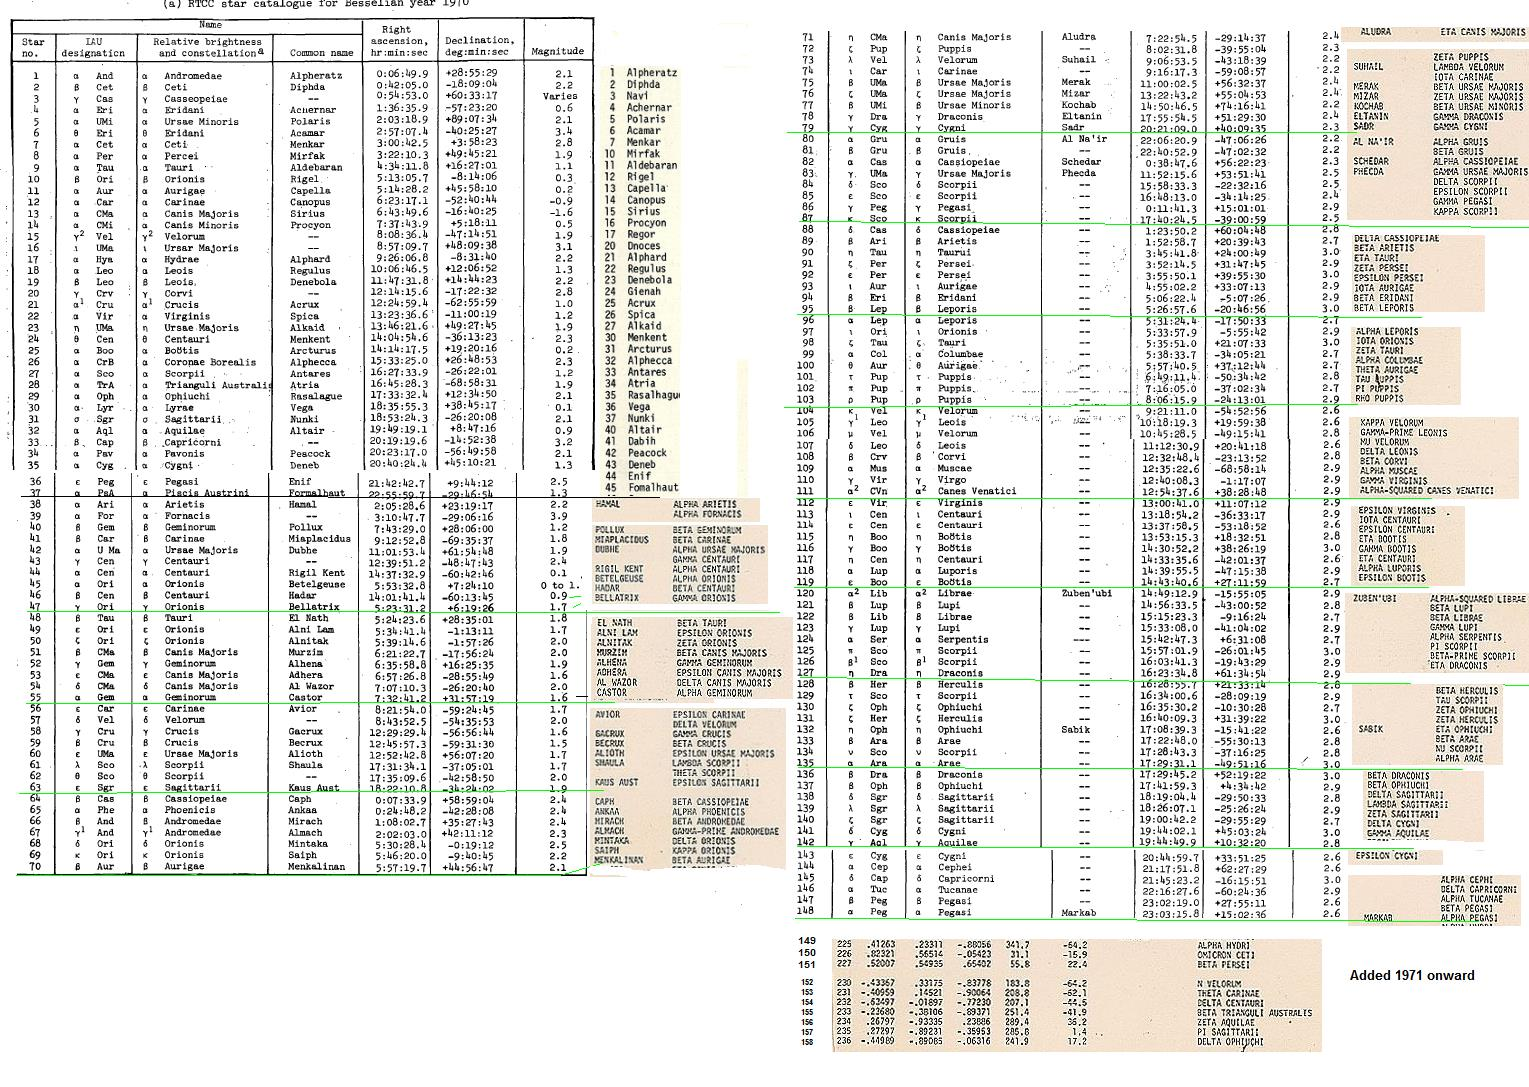
\includegraphics[width=1.3\textwidth]{./ApolloRTCCMFDFiles/Apollo RTCC STARS.jpg}
	\caption{Apollo RTCC Star Catalog}
	\label{fig:RTCCStars}
\end{figure}
\end{landscape}
\newpage
\subsection{Groundtrack Digitals Display (MSK 0347)}
This display shows subsatellite information for a designated vehicle to aid in determining recovery areas. The display is initialized only by input. On entry of a vehicle, revolution (or threshold time) and longitude the display program will compute one-degree increments of longitude for the next 40 degrees beginning with the input longitude. With each longitude thus generated will be computed and displayed a latitude, GET, GMT and true anomaly of the vehicle at the GMT. This is a paging display, yielding a maximum of two pages (20 lines per page).\\

The display is available only in Earth Orbit and Lunar Orbit phases. No automatic updates are provided. An appropriate error message is displayed if any
procedural or processing error is encountered.\\

The display is only available in NASSP with the Mission Plan Table initialized.\\
\newpage
\subsection{Spacecraft Pointing Display (MSK 1504)}
\subsubsection{Function}
To provide mission controllers with pointing angles that will allow the crew to point a spacecraft instrument at an orbiting, celestial or ground target for the purpose of obtaining experimental data.
\subsubsection{Inputs}
Three manual entries are required for this display:
\begin{enumerate}
\item Target specification MED consisting of MODE, INSTRUMENT, TARGET, LAT, LONG, ALT, RA, DEC, REFSMMAT, AT REF, AND DOCKING ANGLE.
\item Initialization MED consisting of T1, T5, and T START. T1 and T5 causes generation of pointing data. T START is for AOS/LOS search.
\item Instrument definition and geometry MED specifying instrument code, code to add or delete. Rl counterclockwise rotation about X Body (Angle out of X-Z plane), R2 counterclockwise rotation about Y Body (Angle out of Y-Z plane). If R1and R2 equal zero the LOS is along the vehicle Z-axis.
\end{enumerate}
\textbf{Target specification:}\\

\textbf{MODE:} 1 = Earth/Moon ground target, 2 = general celestial, 3 = GOST star, 4 = orbiting object.\\
\textbf{INST ID:} Instrument ID. The last 3 characters must be CSM or LEM.\\
 \textbf{ITARGET NM:} Target code.  Mode 1: The last character is E or M. Mode 3: The last 3 characters are a valid star number. Mode 4: Enter 7 characters. Last 3 are CSM or LEM. The first 4 spaces in the TARGET code are for experiment identification and no computations are based upon them.\\
\textbf{LAT:} Latitude of ground target, degrees (Mode 1).\\
\textbf{LNG:} Longitude of ground target, degrees (Mode 1).\\
\textbf{HT:} Height of ground target, nautical miles (Mode 1).\\
\textbf{RT ASC:} Right of ascension of input celestial target (Mode 2).\\
\textbf{DEC:} Declination of input celestial target (Mode 2).\\
\textbf{MATRIX:} Valid REFSMMAT code.\\
\textbf{ATREF:} Attitude reference. IMCSM = CSM IMU, IMLEM = LM IMU, FDLEM = FDAI LM.\\
\textbf{DOK:} Docking angle. Used when instrument vehicle and attitude reference vehicle are not the same.\\
\newpage
\subsubsection{Display}
\begin{center}
\begin{tabular}{ L{2.4cm} L{7.1cm} L{3cm} }
\underline{QUANTITY} & \underline{DEFINITION} & \underline{DIMENSIONS} \\
INST&ID of instrument to be pointed at target&\\
TARGET&Alphanumeric identification code of target&\\
LAT, LNG&Geodetic latitude and longitude of earth target or selenographic latitude and longitude of moon target for MODE 1. Subsatellite position of target vehicle with respect to its reference body in MODE 4 at T1&degrees\\
ALT&Altitude of earth target above oblate body or of moon target above spherical body in MODE 1. Altitude of vehicle target above its reference body in MODE 4 at T1&nautical miles\\
REV&Revolution in which AOS occurs&\\
RA&Right ascension of a celestial target&hr:min:sec\\
DEC&Declination of a celestial target&deg:min:sec\\
AOS&GET and GMT of acquisition of target&hr:min:sec\\
MODE&One of four modes in which display is being used&\\
LOS&GET and GMT of loss of target&hr:min:sec\\
ROLL, PITCH, YAW&Attitudes required of the spacecraft in order to point the line-of-sight of the specified instrument to the target. Displayed for T1 through T5. Attitudes will be as nearly heaas up as possible to the body containing ground target. For other targets, attitudes will be as nearly heads up as possible to the reference body at the time of sighting&degrees\\
AT REF&Code to indicate that the displayed attitudes are referenced to the CSM IMU, the LM IMU, or the LM FDAI&\\
DR, DP, DY&Differences in roll, pitch and yaw between time intervals&degrees\\
EL&Elevation angle of the spacecraft from a ground target. Displayed for T1 through T5&degrees\\
ALT&Spacecraft altitude in nautical miles above spherical reference body. Displayed for T1 through T5&nautical miles\\
RNG&Slant range to ground target. Displayed for T1 through T5&nautical miles\\
\end{tabular}
\end{center}

\begin{center}
\begin{tabular}{ L{2.4cm} L{7.1cm} L{3cm} }
\underline{QUANTITY} & \underline{DEFINITION} & \underline{DIMENSIONS} \\
SUN ANG&The angle in degrees between the spacecraft-sun-line and the instrument line-of-sight Displayed for T1 through T5&degrees\\
MOON ANG&The angle in degrees between the spacecraft-nearest moon horizon-line and the instrument line-of-sight. Displayed for T1 through T5&degrees\\
EARTH ANG&The angle in degrees between the spacecraft-nearest earth horizon-line and the instrument line-of-sight. Displayed for T1 through T5&degrees\\
T1,T2,T3,T4,T5&Evenly spaced times from T1 to T5 at which attitude data are generated&hr:min:sec\\
REFSMMAT&Identification code of REFSMMAT used in generating the display&\\
RA, DEC&Direction of CSM +X-axis if INST is CSM type. Direction of LM +Z-axis if INST is LM type&\\
STAR&Identification code of star in COAS field-of-view at T1 (CSM COAS of CSM INST is specified, LM COAS if LM INST is specified)&\\
SPA&COAS star-pitch-angle for CSM, COAS elevation angle for LM&degrees\\
SXP&COAS star-X-position&degrees\\
\end{tabular}
\end{center}
\newpage
\subsection{Recovery Ascending Node Display (MSK 1505)}
This program displays the time (GET and GMT) of the ascending node, the longitude of the node and the right ascension for the current rev and reach rev within the requested span. Alternative a beginning time and ending time can be input to define this span.\\

The display is available for Earth (ECT) and Moon (MCT) ascending node crossings. In lunar orbit the additional option exists to compute the inertial ascending node crossing time (MCI) instead of the equator crossing. The right ascension display does not apply to lunar orbit however. No automatic updates are provided. An appropriate error message is displayed if any procedural or processing error is encountered.\\

The display is only available in NASSP with the Mission Plan Table initialized.\\
\newpage
\subsection{Vector Comparison Display (MSK 1590)}

\subsubsection{Function}

The Vector Comparison Display shows the local spherical elements, the classical elements and UVW coordinates for a base (first) vector. The differences between the elements of this vector and the second, third, and fourth vectors (if input) will then be computed. From one to four vectors can be specified for comparison. Any available state vector in the evaluation or usable vector tables can be used (see Vector Panel Summary).\\

The UVW coordinate system, essentially a local vertical, local horizontal coordinate system, is defined as follows:

\begin{itemize}
	\item X Axis (U): Vector pointing in the direction of the spacecraft's position vector\\
	\item Y Axis (V): Vector perpendicular to the x- and z-axes, pointing in the direction of travel for a circular orbit\\
	\item Z Axis (W): Vector pointing in the direction normal to the orbit (along the angular momentum vector)\\
\end{itemize}

\subsubsection{Buttons}

\textbf{TIM:} Time of comparison. GMT is assumed if input is positive, GET if negative. Time of V1 vector will be used for comparison if zero is used as the input time.\\
\textbf{VEH:} Vehicle for the comparison. Only relevant if mission planning mode is active in the MFD and an ephemeris vector was chosen.\\
\textbf{V1:} Choose ID of first (base) vector from vector panel summary.\\
\textbf{V2:} Choose ID of second state vector.\\
\textbf{V3:} Choose ID of third state vector.\\
\textbf{V4:} Choose ID of fourth state vector.\\

\textbf{CLC:} Calculate display parameters.\\
\textbf{REF:} Reference body (Earth or Moon) for the comparison values.\\
\textbf{BCK:} Back to last menu\\

\newpage
\begin{landscape}
\subsubsection{Display Parameters}

\begin{center}
\begin{tabular} { L{1cm} L{8cm} L{2cm} L{6cm} }
\hline
Name & Definition & Unit & Comment\\
\hline
H\textsubscript{a} & Keplerian height of apogee (1st column); difference in height of apogee from reference vector (2nd through 4th columns) & n.mi.&Cannot be computed for hyperbolic or parabolic orbits.\\
H\textsubscript{p} & Keplerian height of perigee (1st column); difference in height of perigee from reference vector (2nd through 4th columns) & n.mi.&Cannot be computed for parabolic orbits.\\
V&Inertial velocity magnitude (1st column); difference in velocity from reference vector (2nd through 4th columns).&ft/sec&\\
$\gamma$&Flightpath angle (1st column); difference in angle from reference vector (2nd through 4th columns).&deg&\\
$\psi$&Azimuth (1st column); difference in azimuth from reference vector (2nd through 4th columns).&deg&\\
$\phi$&Latitude (1st column); difference in latitude from reference vector (2nd through 4th columns)&deg&\\
$\lambda$&Longitude (1st column);difference in longitude from reference vector (2nd through 4th columns).&deg\\
h&Height above launch pad (Earth) or lunar landing site (1st column);difference in height from reference vector (2nd through 4th columns).&n.mi.&\\
\end{tabular}
\end{center}
\newpage
\begin{center}
\begin{tabular} { L{1cm} L{8cm} L{2cm} L{6cm} }
\hline
Name & Definition & Unit & Comment\\
\hline
a&Semimajor axis (1st column); difference in semimajor axis from reference vector (2nd through 4th columns).&n.mi.&Cannot be computed for parabolic orbit.\\
e&Eccentricity (1st column); difference in eccentricity from reference vector (2nd through 4th columns)&none&\\
i&Inclination (1st column); difference in inclination from reference vector (2nd through 4th columns)&deg&\\
$\omega$\textsubscript{p}&Argument of perigee (1st column);difference in $\omega$\textsubscript{p} from reference vector (2nd through 4th columns)&deg&\\
$\Omega$&Right ascension of the ascending node (1st column);difference in $\Omega$ from reference vector (2nd through 4th columns)&deg&\\
$\nu$&True anomaly (1st column);difference in true anomaly from reference vector (2nd through 4th columns)&deg&\\
UVW&UVW position coordinates of vehicle (1st column);difference in UVW coordinates from reference vector in feet (2nd through 4th columns).&n.mi., ft&Differences are computed in feet\\
$\dot{U}\dot{V}\dot{W}$& velocity components (1st column);difference in UVW velocity from reference vector (2nd through 4th columns).&ft/sec&\\
\end{tabular}
\end{center}

\end{landscape}

\subsection{Vector Panel Summary (MSK 1591)}

\subsubsection{Function}

The Vector Panel Summary will display the ephemeris anchor vector identifications, anchor vector times and current GMT. It will also display the vector identification and time for each vector in a Usable Vector Slot and each vector in an Evaluation Vector Slot. GMT of ullage tailoff are displayed for the last executed maneuver for both vehicles. The time tags of all available telemetry vectors will also be displayed. The display is updated every six seconds, so inputs on the page might not cause an instant change to the display.

\subsubsection{Display Parameters and Buttons}

The left and right half of the display are showing information about state vectors for CSM and LM respectively. The two sides are identical, so the following description applies to both. Each side is divided into several panels: CMC, LGC, AGS, IU, High Speed Radar, Differential Correction (DC) and Last Executed Maneuver. The first four panels show information about state vectors from telemetry and vectors that have been moved to RTCC tables:\\

UV = Usable Vector Table\\
EV = Evaluation Vector Table\\
TH = Telemetry (High Speed)\\
TL = Telemetry (Low Speed)\\

The TL vector slot has not been implemented yet. Pressing the TLM button will get data from all computers whose vehicles is set on the configuration page and save them in the high speed telemetry tables. In reality the telemetry vectors get continually updated if telemetry is received, so for a more permanent saving solution the vectors can be moved to the evaluation vector table with the EV buttons. The vector is then moved to that table, assigned a vector ID and is then available for comparison using the vector compare display (MSK 1590). AGS and IU vectors need to have their specific REFSMMATs established for the transfer to the evaluation table to work. The telemetry vectors are not guaranteed to be valid, so the evaluation vectors were checked before being "moved up" to the usable vector table, which can be done with the UV buttons. Once in the usable vector table the vectors are available for ephemeris updates.\\

The High Speed Radar panel is not currently implemented. It was a vector that is generated automatically at the end of a powered maneuver using radar data and could, if no telemetry vector was available, be a first estimate of the actual cutoff state.\\

Differential Correction (DC) is the state vector derived from long period ground tracking of the spacecraft during coasting flight. In the RTCC MFD it is simply generated with the DC button and entering the name of the vessel in the simulation. The DC panel will then be updated with a vector ID (APIC/APIL for Orbiter API and C/L for the CSM or LM) and a vector time. The HSR and DC vectors are moved directly to the usable vector table.\\

The last panel shows the last executed maneuver in the mission plan table of the vehicle. The displayed times are ullage on and end of the thrust tailoff period after cutoff.\\

To cause an ephemeris update the TUP button on each side can be pressed and then a vector from the usable vector table is chosen to do the update.\\
\subsubsection{Errors}
If any function of the VPS does not work as expected, an error might have occurred. An associated error message will have been written to the on-line monitor display (MSK 1629). Here follows a list of possible error messages:\\

\begin{tabular}{p{3cm} p{10cm}}
\underline{Code}&\underline{Error Description}\\
1&An unrecognizable queue ID was detected.\\
2&Not used.\\
3&Not used.\\
4&The PBI request made was not a valid request (missing information, two sources indicated, etc.).\\
5&Request to move vector to Usable Slot cannot be honored because there is no vector in the corresponding Evaluation Slot.\\
6&Request to move vector to ephemeris update cannot be honored because there is no vector in the corresponding Usable Slot.\\
7&Not used.\\
8&Test of PBI message header failed; improper message was routed to module.\\
9&Unidentifiable vector ID in the S84 MED.\\
10&Vector to be moved to ephemeris update could not be transformed to ECI coordinates.\\
11&Telemetry vector requested by PBI cannot be furnished this mission.\\
12&Not used.\\
13&Not used.\\
14&The matrix to rotate the telemetry vector requested is not available.\\
15&Request is for a telemetry vector that is not available in the collection slot for this type vector.\\
16&Invalid vehicle code from high-speed processor.\\
17&Invalid vector source code from high-speed processor.\\
18&Vector with lunar landing site indicator set cannot be routed to CSM ephemeris update.\\
\end{tabular}
\newpage
\section{Config Files}

The RTCC loads various configuration files to load constants, mission and launch day specific parameters. The files are located at Config\textbackslash ProjectApollo\textbackslash RTCC. To load a set of files for the monthly launch window add e.g. "RTCC\_MISSIONFILES Apollo 11" to the RTCC section of a prelaunch scenario. This will load the mission constants, TLI and SFP files with the names "Apollo 11 Constants.txt", "Apollo 11 TLI.txt" and "Apollo 11 SPF.txt".\\

\subsection{Star Table}

The RTCC star table is stored in the Star Table.txt file. It contains unit vector of all RTCC navigation stars, starting with the star that get used by the Apollo Guidance Computer. The file is equivalent to the RTCC mission table named EZJGSTAR.

\subsection{Mission Constants}

For each Apollo mission a file with mission constants (e.g. "Apollo 8 Constants.txt") is loaded. These numbers are constant for all possible launch days of a mission. They usually are related to hardware or software which doesn't get changed for a different launch day. Some of these parameters are saved and loaded in scenarios.\\

\begin{tabular}{L{3cm} L{7.5cm} L{2cm} L{1.5cm}}
\hline
\textbf{Name} & \textbf{Description} & \textbf{Default Value} & \textbf{Unit}\\
\hline
AGCEpoch & The epoch of the coordinate system used by the Apollo Guidance Computer and the RTCC& 1969 (Apollo 7-10) & Years\\
\hline
TEPHEM0 & Starting date of AGC time keeping. Always midnight July 1st of the year preceeding the epoch year. Only needs to be loaded for Skylark and the fixed 1950 coordinate system & 40038 & Days (MJD)\\
\hline
MCCLEX & Octal LGC address for external DV uplink & 3433 & None\\
\hline
MCCLRF & Octal LGC address for REFSMMAT uplink (and downlink)& 1733 & None\\
\hline
MCCCXS & Octal CMC address for desired REFSMMAT uplink & 306 & None\\
\hline
MCCLXS & Octal LGC address for desired REFSMMAT uplink & 3606 & None\\
\hline
MCCCRF & Octal CMC address for REFSMMAT uplink (and downlink) & 1735 & None\\
\hline
MCCLRF & Octal LGC address for REFSMMAT uplink (and downlink) & 1733 & None\\
\hline
MCLRLS & Octal LGC address for landing site vector uplink (and downlink) & 2022 & None\\
\hline
MCLTTD & Octal LGC address for the time of lunar landing & 2400 & None\\
\hline
MCLABT & Octal LGC address for descent abort constants & 2545 & None\\
\hline
MCCTEP & Octal CMC address for TEPHEM (liftoff time) & 1706 & None\\
\hline
MCLTEP & Octal LGC address for TEPHEM (liftoff time) & 1706 & None\\
\hline
PZREAP\_RRBIAS & Relative range override for the Return-to-Earth processor & 1285.0 & Nautical Miles\\
\hline
PZREAP\_IRMAX & Maximum return inclination for the Return-to-Earth processor & 40.0 & Degrees\\
\hline
CSMPadLatitude & Geodetic latitude of the CSM launch pad used for launch and IU REFSMMAT calculation & 28.608202 (LC-39A) & Degrees\\
\hline
CSMPadLongitude & Longitude of the CSM launch pad & -80.604133 (LC-39A) & Degrees\\
\hline
LMPadLatitude & Geodetic latitude of the LM launch pad used for IU REFSMMAT calculation & 28.531445 (LC-37B) & Degrees\\
\hline
LMPadLongitude & Longitude of the LM launch pad & -80.565077 (LC-37B) & Degrees\\
\hline
MCTVEN & S-IVB LH2 venting scale factor & 1.0 & None\\
\hline
\end{tabular}

\newpage
\begin{tabular}{L{3cm} L{7cm} L{2.5cm} L{1.5cm}}
\hline
\textbf{Name} & \textbf{Description} & \textbf{Default Value} & \textbf{Unit}\\
\hline
PDI\_v\_IGG & PDI ignition algorithm velocity & 5545.46 & Feet per second\\
\hline
PDI\_r\_IGXG & PDI ignition algorithm x-axis position & -130519.86 & Feet\\
\hline
PDI\_r\_IGZG & PDI ignition algorithm z-axis position & -1432597.3 & Feet\\
\hline
PDI\_K\_X & PDI ignition algorithm coefficient & 0.617631 & None\\
\hline
PDI\_K\_Y & PDI ignition algorithm coefficient & 0.755e-6 & Feet per Feet$^2$\\
\hline
PDI\_K\_V & PDI ignition algorithm coefficient & 410.0 & Seconds\\
\hline
PDI\_RBRFG & PDI braking phase position target & 171.835, 0.0, -10678.596 & Feet\\
\hline
PDI\_VBRFG & PDI braking phase velocity target & -105.876, 0.0, -1.04 & Feet per second\\
\hline
PDI\_ABRFG & PDI braking phase acceleration target & 0.6241, 0.0, -9.1044 & Feet per second$^2$\\
\hline
PDI\_JBRFGZ & PDI braking phase jerk & -0.01882677 & Feet per second$^3$\\
\hline
PDI\_RARFG & PDI approach phase position target & 111.085, 0.0, -26.794 & Feet\\
\hline
PDI\_VARFG & PDI approach phase velocity target & -4.993, 0.0, 0.248 & Feet per second\\
\hline
PDI\_AARFG & PDI approach phase acceleration target &  -0.2624, 0.0, -0.512 & Feet per second$^2$\\
\hline
PDI\_JARFGZ & PDI approach phase jerk & 0.00180772 & Feet per second$^3$\\
\hline
MGVDGD&DPS engine gimbal plane in LM coordinates&154&Inches\\
\hline
MGVSGD&SPS engine gimbal plane in CSM coordinates&833.2&Inches\\
\hline
MGVSTD&Distance between SPS and DPS gimbal planes&435.55&Inches\\
\hline
MCVDKA&Nominal docking angle&240&degrees\\
\hline
MHVCCG&CSM CG table. Format: entry in table, weight, x, y and z coordinates. Example: 0 26600.0 976.946643 0.614894 3.200135&&-, lbs, in, in, in\\
\hline
MHVCCG\_N&Number of entries in CSM CG table&20&\\
\hline
MHVLCG&LM CG table. Format: entry in table, weight, x, y and z coordinates. Example: 0 14000.0 222.73 0.0 0.0&&-, lbs, in, in, in\\
\hline
MHVLCG\_N&Number of entries in LM CG table&40&\\
\hline
MHVACG&LM ascent stage CG table. Format: entry in table, weight, x, y and z coordinates. Example: 0 5000.0 260.9969 0.3187 5.0043&&-, lbs, in, in, in\\
\hline
MHVACG\_N&Number of entries in LM ascent stage CG table&14&\\
\hline
\end{tabular}

\newpage
\begin{tabular}{L{3cm} L{7cm} L{2.5cm} L{1.5cm}}
\hline
\textbf{Name} & \textbf{Description} & \textbf{Default Value} & \textbf{Unit}\\
\hline
MHTSTC&SPS thrust table&20500 lbf and 65.27 lbs &lbf and lbs/sec\\
\hline
MHTSTC\_N&Number of entries in SPS thrust table&1&\\
\hline
MHTATC&APS thrust table&3439 lbf and 11.31 lbs/sec&lbf and lbs/sec\\
\hline
MHTATC\_N&Number of entries in APS thrust table&1&\\
\hline
MHTDTC&DPS thrust table&9712.5 lbf and 32.27 lbs/sec&lbf and lbs/sec\\
\hline
MHTDTC\_N&Number of entries in DPS thrust table&1&\\
\hline
MGTESE&Number of tesseral and sectorial coefficients in Earth potential&0 (use 4 in Open Orbiter)&\\
\hline
MMTESE&Number of tesseral and sectorial coefficients in Moon potential&0 (use 3 in Open Orbiter)&\\
\hline
LAZCOE&Saturn IB launch targeting launch azimuth polynomial& 8568.36235 -20.131 -1.2501 5.5863385&\\
\hline
\end{tabular}
\newpage
\subsection{Launch Day Init Parameters}

For each launch day of a given mission (e.g. "1968-12-21 Init.txt" for Apollo 8) a few parameters are being loaded as initial values. These parameters are almost all saved and loaded and may be overwritten during a mission, so they are only loaded from file once when the RTCC is first being started.\\

\begin{tabular}{L{3.7cm} L{7cm} L{1.95cm} L{1.5cm}}
\hline
\textbf{Name} & \textbf{Description} & \textbf{Default Value} & \textbf{Unit}\\
\hline
LDPPDwellOrbits & Number of dwell orbits desired between DOI and PDI used by the Lunar Descent Planning Processor & 0 & None\\
\hline
LDPPDescentFlightArc & Powered flight arc of descent for the Lunar Descent Planning Processor & 15.0 & Degrees\\
\hline 
LDPPHeightofPDI & Height of PDI used by the Lunar Descent Planning Processor & 50000.0 & Feet\\
\hline
PZLOIPLN\_HP\_LLS & Height of perilune at PDI for the LOI Targeting & 8.23 & Nautical Miles\\
\hline
TLCC\_AZ\_min & Minimum approach azimuth to the landing site used by the Translunar Midcourse Processor & -110.0 & Degrees\\
\hline
TLCC\_AZ\_max & Maximum approach azimuth to the landing site used by the Translunar Midcourse Processor & -70.0 & Degrees\\
\hline
REVS1 & Number of orbits between LOI-1 and LOI-2 (or DOI for the later missions) used by the TLMCC and LOI targeting & 2.0 & None (double)\\
\hline
REVS2 & Number of orbits between LOI-2 (or DOI for the later missions) and PDI used by the TLMCC and LOI targeting & 11 & None (Integer)\\
\hline
LOPC\_M & Number of revolutions from first pass over lunar landing site to lunar orbit plane change maneuver. Used by LOPC routine of the TLMCC processor & 3 & None\\
\hline
LOPC\_N & Number of revolutions from lunar orbit plane change maneuver to second pass over lunar landing site. Used by LOPC routine of the TLMCC processor & 8 & None\\
\hline
\end{tabular}

\begin{tabular}{L{3.7cm} L{7cm} L{1.95cm} L{1.5cm}}
\hline
\textbf{Name} & \textbf{Description} & \textbf{Default Value} & \textbf{Unit}\\
\hline
LOI\_psi\_DS & Desired approach azimuth to the lunar landing site. Used by the LOI targeting & 270.0 & Degrees\\
\hline
eta\_1 & True anomaly on LPO-1 (orbit after LOI-1) for transferring from the hyperbola to LPO-1. Used by TLMCC and LOI targeting & 0.0 & Degrees\\
\hline
H\_P\_LPO1 & Perilune height on LPO-1 (orbit after LOI-1). Used by TLMCC and LOI targeting & 60.0 & Nautical miles\\
\hline
PZLTRT\_DT\_Ins\_TPI & Time between insertion and TPI for the short rendezvous profile in lunar orbit & 40.0 & Minutes\\
\hline
SITEROT & Angle of perilune from the lunar landing site (negative if the site is post-perilune). Used by the TLMCC and LOI targeting & -15.0 & Degrees\\
\end{tabular}

\newpage
\subsection{Skeleton Flight Plan Table}

The skeleton flight plan table is a table of initial guesses for the translunar midcourse correction processor. The files are specific to the monthly launch window and contain up to 10 days of data. The file names are usually something like "Apollo 11 SFP.txt". The format of the file follows the MSC card format from the MSC internal note RTCC REQUIREMENTS FOR APOLLO 11 (MISSION G) PREFLIGHT INFORMATION (69-FM-171), which can be found \href{https://web.archive.org/web/20100524010957/http://ntrs.nasa.gov/archive/nasa/casi.ntrs.nasa.gov/19740072570_1974072570.pdf}{here}. PDF page 13 shows the general format of one data set. One line in the config file is equal to one punch card. Some adaptions have been made for the additional parameters needed on hybrid missions. The complete format for one data set is:\\

\begin{tabular}{|L{2.9cm}|L{2.9cm}|L{2.8cm}|L{2.8cm}|L{1.4cm}|}
\hline
Day (1 to 366)&Opportunity (1 or 2)&Launch azimuth (deg)&Launch window (A or P)&Card ID\\
\hline
Latitude of TLI pericynthion (deg)&Longitude of TLI pericynthion (deg)&Height of TLI pericynthion (NM)&GET of TLI (hours)&Card ID\\
\hline
Latitude of LOI pericynthion (deg)&Longitude of LOI pericynthion (deg)&Height of LOI pericynthion (NM)&&Card ID\\
\hline
dpsi of LOI (deg)&gamma of LOI (deg)&Time in lunar orbit (hrs)&Time from LOI to landing (hrs)&Card ID\\
\hline
Approach azimuth (deg)&Latitude of the landing site (deg)&Longitude of the landing site (deg)&Radius of the landing site (NM)&Card ID\\
\hline
dpsi of TEI (deg)&DV of TEI (ft/s)&time from TEI to EI (hrs)&Inclination of free return (deg)&Card ID\\
\hline
GMT of TLI pericynthion (hrs)&GMT of LOI pericynthion (hrs)&GMT of node (hrs)&&Card ID\\
\hline
Latitude of node (deg)&Longitude of node (deg)&Height of node (NM)&&Card ID\\
\hline
\end{tabular}

\newpage
\subsection{TLI Targeting Parameters}

The files containing the TLI targeting parameters follow the launch day specific format "`1968-12-21 TLI.txt". They contain the numbers needed to calculate the time of restart preparations and the TLI maneuver in the RTCC. The format of the file follows the MSC card format from the MSC internal note RTCC REQUIREMENTS FOR APOLLO 11 (MISSION G) PREFLIGHT INFORMATION (69-FM-171), which can be found \href{https://web.archive.org/web/20100524010957/http://ntrs.nasa.gov/archive/nasa/casi.ntrs.nasa.gov/19740072570_1974072570.pdf}{here}. The PDF pages 32 to 40 show the format. One line in the config file is equal to one punch card.


\newpage
\subsection{Erasable Memory Programs}

Erasable Memory Program (EMP) files are loaded in the EMPs folder, which is under Config/ProjectApollo/RTCC. They contain uplink data for the CMC and LGC. The format of the file is as follows:\\

\begin{itemize}
\item The first line contains a description of the EMP which is shown on the uplink MFD page.
\item The second line contains the AGC rope name (e.g. Luminary 210) for which the EMP is valid.
\item The actual uplink loads follow in the subsequent lines. Each load has two lines in the file and the number of possible loads per file is not limited. There are two types of EMP uplinks. Contiguous block update (Verb 71) updates from 1 to 18 consecutive erasable memory registers in the same erasable memory bank. The scatter update (Verb 72) provides the capability to update from 1 to 9 non-consecutive erasable memory registers in the same or different erasable memory banks. The first of the two lines in each load contains either 71 and the starting address for Verb 71 or 72 and no additional value for Verb 72. The second line then contains all the uplink data, for Verb 72 it is alternating address and value. All data is in octal.
\end{itemize}

On the next page follows a list of EMPs that come with NASSP:\\
\newpage

\begin{tabular}{|l|L{9cm}|l|}
\hline
\textbf{EMP Filename}&\textbf{Description}&\textbf{Rope}\\
\hline
P99 L1D&Guided RCS Translation Maneuver&Luminary 178\\
\hline
EMP 99&Guided RCS Translation Maneuver&Luminary 210\\
\hline
EMP 100A&Backup for failed DSKY key using engine gimbal switch&Luminary 210\\
\hline
EMP 100B&Backup for failed DSKY key using mode sel switch&Luminary 210\\
\hline
EMP 103A&Descent with failed CDUs&Luminary 210\\
\hline
EMP 103B&EMP for failed CDUX&Luminary 210\\
\hline
EMP 108&Zero a runaway IMU CDU and prevent coarse align&Luminary 210\\
\hline
EMP 500&Landmark Tracking With Datalink Failure Or Unusable Optics&Artemis 72\\
\hline
EMP 501&Landmark Tracking With Failed Mark/Mark Rej Button&Artemis 72\\
\hline
EMP 512&P40/41/47 Termination During Average G When EMP 509 is Operating&Artemis 72\\
\hline
EMP 514&Shortened P23&Artemis 72\\
\hline
EMP 515&Manual Range Input&Artemis 72\\
\hline
EMP 517&Convert Optics Shaft And Trunnion Angles To Body Angles&Artemis 72\\
\hline
EMP 523&Monitor Jet-On Failure&Artemis 72\\
\hline
EMP 525A&Optics Switch Monitor&Artemis 72\\
\hline
EMP 526 (1 Deg)&IMU CDU Transient Monitor (1 Degree Check)&Artemis 72\\
\hline
EMP 526 (2 Deg)&IMU CDU Transient Monitor (2 Degree Check)&Artemis 72\\
\hline
EMP 526 (3 Deg)&IMU CDU Transient Monitor (3 Degree Check)&Artemis 72\\
\hline
EMP 526 (4 Deg)&IMU CDU Transient Monitor (4 Degree Check)&Artemis 72\\
\hline
EMP 527 (CDUX)&Monitor Single IMU CDU (CDUX)&Artemis 72\\
\hline
EMP 527 (CDUY)&Monitor Single IMU CDU (CDUY)&Artemis 72\\
\hline
EMP 527 (CDUZ)&Monitor Single IMU CDU (CDUZ)&Artemis 72\\
\hline
EMP 528&Monitor Jet-On Failure and Do EMP 526&Artemis 72\\
\hline
EMP SL-15&Manual Range Input&Skylark 48\\
\hline
EMP SL-23&Monitor Jet-On Failure&Skylark 48\\
\hline
EMP SL-26 1 Deg&IMU CDU Transient Monitor (1 Degree Check)&Skylark 48\\
\hline
EMP SL-26 2 Deg&IMU CDU Transient Monitor (2 Degree Check)&Skylark 48\\
\hline
EMP SL-26 3 Deg&IMU CDU Transient Monitor (3 Degree Check)&Skylark 48\\
\hline
EMP SL-26 4 Deg&IMU CDU Transient Monitor (4 Degree Check)&Skylark 48\\
\hline
EMP SL-27 CDUX&Monitor Single IMU CDU (CDUX)&Skylark 48\\
\hline
EMP SL-27 CDUY&Monitor Single IMU CDU (CDUY)&Skylark 48\\
\hline
EMP SL-27 CDUZ&Monitor Single IMU CDU (CDUZ)&Skylark 48\\
\hline
EMP SL-28&Monitor Jet-On Failure and Do EMP SL-26&Skylark 48\\
\hline
EMP SL-50&Convert Gyro Torquing Angles to CDU Angles for Failed CDU&Skylark 48\\
\hline
EMP SL-52A&Checksum for VAC area 4 for EMP SL-23&Skylark 48\\
\hline
EMP SL-52B&Checksum for VAC area 4 for EMP SL-28&Skylark 48\\
\hline
EMP SL-55&IMU Slip Ring Program&Skylark 48\\
\hline
EMP ASTP-75&Compute S-Band Antenna Angles&Skylark 48\\
\hline
EMP ASTP-77&Raster Scan&Skylark 48\\
\hline
\end{tabular}

\end{document}
